% Documentation:
%
% The UoK class file extends the standard report style to follow the Registry
% guidelines for laying out a thesis. It sets the margins, interline spacing,
% the page, figure and table numbering style, and disallows page breaks at
% hyphens. The class file consists of setting one and an half line spacing text
% with a 4cm left margin, at least a 2.5cm right margin, approximately 2cm top
% and bottom margin, on A4 paper.
% 
% The class the following options, in addition to those of the standard report
% class.
%     mini - Toggles the thesis in to mini-thesis mode. This adds "mini" to the
%            title and appends a nocite(*) at the end for an automatic output of
%            your complete bibliography.
%     draftmark - Puts a DRAFT' watermark on every page of the document along
%                 with the draft statement on the title page. Additionaly, it
%                 is used as a switch for the UoKExtentions package.
%     draft - Puts the entire document into draft mode. Applies all the effect
%             of draftmark above, but also propergates to other packages used.
%     copyright - Adds a copyright page between the title page and the preface.
%     nofig - Disables output of the list of figures in the preface.
%     notab - Disables output of the list of tables in the preface.
% All options passed to UoKthesis will be passed along to included packages:
%    natbib, draftwatermark, setspace, hyperref, lmodern
%
% The cover page and optional copyright page are implicitly added before the
% start of the preface section. Use the following commands to populate the 
% cover page/copyright page information:
%     \title{thesis title}
%     \author{author's name} 
%     \degree{Master of Science, Doctor of Philosophy, etc.} 
%     \subject{author's department}
%          - Computer Science if omitted 
%     \submitdate{month year in which submitted}
%          - dated by LaTeX if omitted 
%     \copyrightyear{year degree conferred (next year if submitted in Dec.)}
%          - assumes current year (or next year, in December) if omitted 
% 
% The preface environment allows for the use of sections that precede the main
% document; such as Abstract and  Acknowlegements. These sections should be
% defined using \section{Preface Section Title}. The contents page (and list of
% figures and tables if in use) will be automatically inserted at the end of the
% preface environment.
%
% The thesis style invokes the setspace package to set the commands:
%     \doublespace
%     \onehalfspace
%     \singlespace
% for spacing. By default one and an half spacing is used which resembles the
% UKC Typewriter requirement. Singlespace can be used for letterpress
% appearance. If you want to use true double space, for some reason, place the
% \doublespace command where you want to start using double spacing. Just call
% the appropriate spacing command at where you want to use them.
% 
% In the figure and table environments, single spacing is used. If you want to
% use any other size rather than one and an half spacing, then do:
% 	\renewcommand{\baselinestretch}{1.6} (or whatever you want instead of 1.6)
% This command won't take effect unless it comes before the \begin{document} or
% is triggered by a font change (after something like \small \normalsize).
%
% The example below shows the 12pt thesis style being used. This seems to give
% acceptable looking results, but it may be omitted to get 10pt. Alternatively,
% the 11pt option can be used.
%
% This version differs from old_ukcthesis.sty in the following ways:
% 1. Removed the doublespace package (now uses setspace).
% 2. Merged the phantom section for correct PDF links into the bibliography
%    generating function. 
% 3. Added thesis type options (mini, draft).
% 4. Kent Harvard is used for referencing and citation, this is supported by the
%    natbib package.
% 5. PsFig macro removed.
% 6. Now comes as two files, UoKthesis.cls, which defines purely stylistic layout,
%    and UoKextentions.sty, that provideds some additional functionality.

\documentclass[12pt]{UoKthesis}

%\renewcommand*\rmdefault{ptm}
%\renewcommand{\familydefault}{\rmdefault}
% Note: The UoKextentions package includes the xcolor package with the [usenames]
% options. If you need to add further options, these can be given to UoKextentions
% to be propogated through.
\usepackage{UoKextentions}
\usepackage{times}
%\usepackage{llncsdoc}
%\usepackage{verbatim}
\usepackage{url}
\usepackage{color}
\usepackage{adjustbox}
\usepackage{amsmath}
\usepackage{relsize}
\usepackage[final]{listings}
\usepackage[T1]{fontenc}
%\usepackage[math]{times}
\usepackage{mathptmx}
\usepackage{graphicx}
\usepackage{wrapfig}
\usepackage[scaled=.90]{helvet}
\usepackage{courier}
\newcommand{\td}[1]{{\bf {\tt{#1}}}}
\newcommand{\comment}[1]{\textcolor{red}{\td{{#1}}}}
\usepackage{textcomp}
\usepackage{csquotes}
\lstset{
  frame=none,
  xleftmargin=2pt,
  stepnumber=1,
  numbers=left,
  numbersep=5pt,
  numberstyle=\ttfamily\tiny\color[gray]{0.3},
  belowcaptionskip=\bigskipamount,
  captionpos=b,
  escapeinside={*'}{'*},
  language=haskell,
  tabsize=2,
  emphstyle={\bf},
  commentstyle=\it,
  stringstyle=\mdseries\ttfamily,
  showspaces=false,
  keywordstyle=\bfseries\ttfamily,
  columns=flexible,
  upquote=true,
  showstringspaces=false,
  basicstyle=\small\ttfamily,
  breaklines=true,
  morecomment=[l]\%,
}

% Kent Harvard Bibliography Style. WIP
\bibliographystyle{kentHarvard}

% Provides nice linking in PDFs
\usepackage{hyperref}

% Only needed if you want to produce an index. Example is shown at the bottom of this document.
\usepackage{makeidx}

% Useful packages
% \usepackage{epstopdf} % Converts EPS files to PDF using ghostscript
% \usepackage{fnbreak}  % Warns you if you have split footnotes
% \usepackage{mathpazo} % Type­set­ math­e­mat­ics in the Palatino fam­ily of text fonts
% \usepackage{paralist} % Enumerate and itemize within paragraphs
% \usepackage{amsmath}  % AMS mathematical facilities
% \usepackage{rotating} % Rotating facilities for floats

\usepackage{caption}
\usepackage{subcaption}
\setcounter{secnumdepth}{3} % add more section types

%%%%% macros
\def\fixme#1{\fbox{\textbf{\textsc{Fixme}}\quad#1}}
\def\fixpic#1{\fbox{\textbf{\textsc{Picture}}\quad#1}}
\def\defnx#1#2{\emph{#1}\index{#2}}
\def\defn#1{\defnx{#1}{#1}}
\def\floatpic#1#2{%
\begin{wrapfigure}{r}{\dimexpr #1 / 2 \relax}
\includegraphics[width=\dimexpr #1 / 2 \relax]{#2}
\end{wrapfigure}}
\def\inlinepic#1#2{%
\begin{center}
\includegraphics[width=\dimexpr #1 / 2 \relax]{#2}
\end{center}}

%%%%% augment hyphenation
\hyphenation{wide-spread}

%%%%% document start
\begin{document}

\title{Data-Driven Refactorings for Haskell}
\author{Stephen Adams}
\subject{Computer Science}
\degree{PhD}

\begin{preface}
\section{Abstract}

Refactoring is the process of changing the internal structure of a program without changing its external behaviour. The goal of performing refactorings is to increase code quality. However, refactoring by hand is time consuming and error-prone. This makes automated refactoring tools very useful.

Agile software development allows for software to evolve slowly over time. This evolution changes how a program processes, abstracts over, and views its data. This evolution, though necessary, comes with the cost of technical debt. As technical debt increases changes to a code base become more difficult. Refactoring is one of the primary ways to  reduce technical debt. 

There exist refactorings that specifically help software to evolve its data model, however these refactorings are specific to the object-oriented programming paradigm. Haskell is a strongly typed, pure functional programming language. Haskell's rich type system allows for complex and powerful data models and abstractions. This thesis reports on work done to design and automate refactorings that help Haskell programmers develop and evolve these abstractions.

This work also discussed the current design and implementation of HaRe (the \textit{Ha}skell \textit{Re}factorer). HaRe now supports the Glasgow Haskell Compiler's implementation of the Haskell 2010 standard and its extensions, and uses some of GHC's internal packages in its implementation. 

\section{Acknowledgements}
First I would like to thank my supervisor Professor Simon Thompson, for his guidance and patience throughout this process. Without his help this thesis would not have been possible.

I also need to thank my parents, Jeff and Diane, for their support and encouragement. You both have been so excited for me to take this opportunity. It can't have been easy to have me live an ocean away, and your support in me started this project has been amazing.

A special thanks go out to Kristin Lamberty, Elena Machkasova, and Nic McPhee the professors of computer science at the University of Minnesota, Morris. All three of you introduced me to the world of computing and I wouldn't be here today without all of your help. You prepared me as much as anyone can be prepared for a PhD.

Alan Zimmerman is cited many times in this thesis but I don't think that is sufficient thanks for all the work he has done. Without you HaRe would not be where it is today. You dedication to the Haskell open source community is much appreciated.

I would like to extend my thanks to Adriana and Gaya Perera for letting me stay with them for the final year of my degree. You very graciously opened your house to me when I needed it and allowed me to stay much longer than any of us were expecting.

Finally I must thank Rosemary for her love and support. You have supported me through some of the toughest times of my life. Without you this would not have been finished, and without you this accomplishment would mean nothing.

\end{preface}

\chapter{Introduction}\label{chp:intro}


\section{Functional Programming}
Functional programming is a programming paradigm that focuses on data values as described by expressions which are built from function applications and definitions~\citep{elementsOfFunc}.  Functions in this case are closely related to the idea of mathematical functions. What qualifies a programming language as functional is debatable but several concepts are often included in languages that are described as functional. 

First class functions mean that functions are allowed to be treated like any other data type. First class functions can be passed to or returned from from other ``higher-order'' functions. Iteration is accomplished through recursion rather than via looping. There is also a heavy emphasis on functions remaining ``pure,'' that is without side effects; though functional languages do provide ways to use IO or state, it is emphasised that functions should remain pure if at all possible. Haskell's type system allows for effectful computations to be contained within monad types.
  
\section{Haskell}
\label{haskell}
Haskell is a statically typed, lazily evaluated, pure functional language. Haskell is strongly and statically typed, and supports Hindley-Milner type inference(\cite{hindley};\cite{milner}). Type inference means that Haskell programs do not need every type to be explicitly listed in the source code. Types will be~\textit{inferred} at compilation time so that every part of a Haskell program's type is known at that time. Haskell's type system also allows users to define their own types.

Lazy evaluation, also known as call-by-need~\citep{wadsworth}, means that Haskell expressions are not evaluated when they are passed as a parameter, but rather when that value is used. For example, in the Haskell function \texttt{f}, in figure~\ref{lazyY}, the parameter y will never be evaluated. Lazy evaluation is more nuanced than call-by-name style parameter passing. Composite data types will be evaluated only as much as required to allow the computation to continue. This allows for both partial and infinite data types, for example \texttt{[1..]} is a list containing all of the natural numbers. 

\begin{figure}[t]
\begin{lstlisting}
f x y = case x > 0 of
True -> x - 1
False -> x + 1
\end{lstlisting}
\caption{A simple function}
\label{lazyY}
\end{figure}

Haskell is also a pure language. Purity is the idea that functions cannot perform actions in addition to returning values. These additional actions are known as side-effects. Haskell allows for traditionally side-effect causing operations (IO, state, etc.) through the use of monads. Monads represent computations, which when run will have effects as well as producing a result. A principle topic of this thesis is refactoring to support patterns of computation related to Monads and other related structures. 

\section{Refactoring} 
Refactoring is the process of changing a program without changing its behaviour. This is done to improve its internal structure~\citep{fowler}. The term refactoring was first coined in~\citep{programRestructuring} and these ideas expanded to the object-oriented paradigm in~\citep{refactOOFrameworks}. People have been performing refactoring for much longer and it was called ``program restructuring'' in the literature(\cite{highSpeedRestructuring}; \cite{performanceRestructuring}). Martin Fowler's 1999 book ``Refactoring'' has become the canonical reference for object-oriented refactorings~\citep{fowler}.

Behaviour preservation is what separates refactoring from other types of program manipulation. This idea of functionality preservation means that refactoring will not introduce new bugs or eliminate old ones. To prevent semantic changes after refactoring, many refactorings have non-trivial preconditions~\citep{mens2002formalising}. For example, the renaming refactoring should check that the new name being introduced does not cause a name clash with a name already used in the source program.

Manual refactoring is tedious and error prone because changes to small portions of code may require system-wide changes. When deleting a parameter from a function, for example, every call site of that function also needs to be modified, and missing even a single call site will cause an error. Refactoring by hand depends on high testing coverage to ensure that functionality is preserved~\citep{fowler}. This means that tools that can automatically perform refactorings and ensure that preconditions are met are highly desirable.

\subsection{Functional refactoring}

Refactoring a functional language has a few key differences from refactoring an imperative language. The higher-order nature of functional languages means that any sub-expression of a function is a candidate for generalisation whereas in other languages the types of parameters and results is limited. This means that functional refactorings can target The semantics of functional languages also allow for more comprehensive checking of preconditions based on the static semantics of the language~\citep{refacTools}.

It is also not unusual for functional refactorings to be substantially different than their object-oriented (OO) counterparts. For example creating a case statement from a multi-equation function definition in a functional language versus inlining a virtual method as a case statement in an OO language require substantially different program manipulations~\citep{huiqingThesis}. Additionally there can be refactorings with no OO counterpart, monadification, the introduction of monadic types into otherwise pure code, for instance.

\section{Summary}

One of the most widely accepted best practices in software development is the concept of incremental change, an essential concept of both the extreme programming and agile software development philosophies (\cite{extremeProg}; \cite{agileManifesto}). Refactoring remains a key step in this incremental development process to preventing technical debt from causing development to slow to a crawl.

Much of the refactoring literature focuses on changes that need to be made to the structure of programs. The structure of a program is very important and structural refactorings can maintain the ``separation of concerns'' by extracting functions from existing definitions or ensuring that a program's names reflect what the program currently does. This thesis argues that it is just as important to maintain the ways that a program structures and evaluates the data it computes.

This thesis has chosen to use the term ``data-driven'' to describe the type of refactorings that are prompted by the data that a program computes. These refactorings can be prompted by an insufficiently fine-grained data model. For example, the ``introduce type synonym'' refactoring which creates a new type synonym that helps separate certain instances of a type that are used to represent different concepts.

This thesis also takes advantage of Haskell's call-by-need evaluation strategy which allows for control flow to be abstracted by the user. The ``generalise monad to applicative refactoring'' (see Chapter~\ref{chp:applicative}) takes code that was formally monadic and sequentially evaluated and makes it possible to evaluate it in parallel. The ``generalise maybe'' refactorings from Section~\ref{genMaybe} takes a concrete effect and makes it an abstract one that can be instantiated in multiple ways. Both of these refactorings are applied as either the programmer's understanding of the data they are working with becomes more nuanced or to prepare the program's data model for enhancement. In this way the data ``drives'' these refactorings.

\section{Thesis Outline}

This thesis will proceed as follows:


\textbf{Chapter~\ref{chp:related}: Related work}

This thesis begins with chapter that discusses the some of the related work that this thesis builds from and is inspired by. 

%%%%%%%%%%%%%%%%%%%%%%%%%%%%%%%
\comment{Update this!!!}
This chapter covers other refactoring tools for other functional and object-oriented languages. This chapter also discusses multiple projects that are using refactoring in unique and interesting ways such as introducing parallelism, and non-traditional programming languages. Next the chapter describes work on developing syntactic sugar for applicative functors. Finally there is a brief discussion of type changing program transformation systems.


\textbf{Chapter~\ref{chp:hare}: Background: Refactoring Haskell in HaRe}

This chapter covers the history of HaRe (the \textbf{Ha}skell \textbf{Re}factorer), the technologies it depends on, and the current implementation of HaRe. Specifically there is an overview of the~\citep{ghcApi}, the generic traversal library Scrap Your Boilerplate~\citep{syb}, and ghc-exactprint~\citep{exactprint}. This chapter also describes how the inner workings of HaRe are implemented and the functions that compose its API. Finally it discuses the design and development process of implementing refactorings for HaRe.

\textbf{Chapter~\ref{chp:ddRefs}: Data-Driven Refactorings}

Chapter~\ref{chp:ddRefs} introduces data-driven refactorings. The chapter begins with a discussion of this type of refactoring for object-oriented languages. The rest of the chapter describes data-driven refactorings for the Haskell programming language. First there is a description of the ``introduce a type synonym,'' the ``renaming'' refactoring of data-driven refactorings. The renaming refactoring is the most straightforward refactoring, it simply changes the name of a variable to one that better suits the real meaning of the variable. Similarly a type synonym can rename types to better reflect what certain instances of that type are being used for in a program, and this refactoring supports that transformation. The other two refactorings covered in this chapter are the ``generalising maybe'' and ``list to Hughes list'' refactorings.

The ``generalising maybe'' refactoring (Section~\ref{genMaybe}) rewrites functions that use the concrete type of \texttt{Maybe} to use, instead, the operations provided by the typeclasses it implements, \texttt{Monad} and/or \texttt{MonadPlus}. The final refactoring described by this chapter is the ``list to Hughes list'' refactoring (Section~\ref{listToDlist}). Hughes lists (also known as difference lists) are an alternative implementation for lists that support $O(n)$ time appends. This refactoring takes functions that use that standard list implementation and rewrites the function to use Hughes lists instead. The approach for this refactoring is applicable between any two types that are ``reversibly embeddable'' a concept that will be defined as well.

\textbf{Chapter~\ref{chp:generalImp}: Implementing Data-Driven Refactorings in HaRe}

This chapter continues from the refactoring designs presented in chapter~\ref{chp:ddRefs} to describe HaRe's implementation of both the ``maybe to MonadPlus'' and the ``list to Hughes List'' refactorings. There is also be a discussion of the API that  supports the ``list to Hughes List'' refactoring and can be used to define further ``reversibly embeddable'' type refactorings. Finally this chapter will describe the enhancements made to HaRe's API, specifically the addition of high-level transformation functions.

\textbf{Chapter~\ref{chp:applicative}: Generalising Monads to Applicative}

This chapter presents another generalisation refactoring. Applicative functors are a, relatively, new addition to the Haskell environment. Applicative functors are an interface for sequencing effectful computations. Currently the Haskell community predominantly uses the monadic interface for effects. This chapter will describe the design and implementation of a refactoring for taking a monadic \texttt{do} statement and transforming it to use the \texttt{Applicative} (the Haskell typeclass for Applicative functors) interface instead.

This chapter also describes how the Haskell community is currently using the \texttt{Applicative} interface, based on the results of a survey of Hackage, the Haskell package archive~\citep{hackage}. Finally this chapter concludes with a discussion of possible applications of the refactoring.

\textbf{Chapter~\ref{chp:monadification}: Introducing Monads} 

Chapter~\ref{chp:monadification} describes the monadification refactoring. Monadification is the process of introducing monads into pure code. Monads are the standard way for effects to be used in Haskell and so a refactoring to automatically add them is very useful to the community. There are many styles of monadification and this chapter describes several of them. Finally it discusses the implementation of the monadification refactoring in HaRe.

\textbf{Chapter~\ref{chp:conc}: Conclusion}

The final chapter summarises the work done for this thesis and the contributions it has made. It concludes with a discussion of future work that could be performed on HaRe.

\section{Contributions of this Research}

The work in this thesis was carried out in HaRe. This study focused on adding additional refactorings to HaRe of a new type. Rather than being motivated by the structural problems of a program, data-driven refactorings seek to resolve issues that are caused by the data types a program uses. The contributions of this research are:

\begin{itemize}
	\item Extending the HaRe API to better support data-driven refactorings. These refactorings are complex and require more information from the abstract syntax of GHC than prior refactorings in HaRe. The contributions to the API were focused on analysis of the types of nodes and creating a higher level interface for common small expression level transformations. These changes are described in Chapter~\ref{chp:generalImp}.
	\item The design and implementation of the ``generalise maybe'' and ``list to Hughes list'' refactoring, described in Chapters~\ref{chp:ddRefs} and ~\ref{chp:generalImp}. The ``generalise maybe'' refactoring is a way of taking a concrete effect and turning it into an abstract one so that it can be instantiated in multiple ways. The ``list to Hughes list'' refactoring describes a way to rewrite  a program's data model to use a different type with a similar interface.
	\item The design and implementation of the ``generalise monads to applicative'' refactoring, Chapter~\ref{chp:applicative}. Effects in Haskell are typically handled using monads, a powerful abstraction that allows the type system to check the type of the effects that are being performed by a program. Since the introduction of monads the Haskell community has developed more fine-grained approaches to effect handling. This refactoring allows software systems to handle effects using the applicative as opposed to the monadic interface.
	\item The design and implementation of the ``monadification'' refactoring, see Chapter~\ref{chp:monadification}. Monadification is the process of making a program work over a monadic type rather than a pure one. This refactoring supports the evolution of pure programs to effectful ones.
\end{itemize}


%%%%%%%%%%%%%%%%%%%%%%%%%%
\chapter{Related Work}
\label{chp:related}

This chapter reviews current work in refactoring and other areas of the literature and helps to situate the work described in this thesis into the broader landscape provided by the literature. This chapter begins with a short description of refactoring tools, both for modern sophisticated IDEs that support object-oriented languages and the refactoring tools that support functional languages. 

Next Sections~\ref{refacParallel} and ~\ref{applicativeDo} will describe some of the work done to transform programs so that they are executed in parallel rather than sequentially. The original idea behind refactoring was to reduce the technical debt of a target program. The potential scope of refactorings have been expanded to include introducing parallelism rather than just improving code quality. 

Section~\ref{typeTrans} covers work done in the program transformation and refactoring fields. In particular earlier versions of monadification are discussed, such as ``Reuse by Program Transformation''~\citep{lammelReuse}, and ``Monadification of Functional Programs''~\citep{monadification}. Other work that is covered in this section includes work on refactoring and program transformation that is particularly focused on types.

The final section of this chapter will discuss how refactoring tools are implemented. This section will pay special attention to refactoring tools that target languages other than Haskell, this is because the focus of Chapter~\ref{chp:hare} is on building refactoring tools for Haskell.

\section{Refactoring Tools in Modern IDEs}\label{ideTools}
Refactoring tools have become a standard feature in integrated development environments. The four most popular IDEs for object-oriented languages, Eclipse\footnote{\url{https://www.eclipse.org/}}, NetBeans\footnote{\url{https://netbeans.org/}}, IntelliJ\footnote{\url{https://www.jetbrains.com/idea/}}, and Visual Studio\footnote{\url{https://www.visualstudio.com/}} all come with refactoring tools for their primary language~\citep{ides}. These refactoring tools support some general (renaming, method extraction) and object-oriented specific refactorings (pushing/pulling methods up/down the object hierarchy). 

\section{Refactoring Tools for functional languages}\label{funcTools}
A reason that often used to be given to explain why functional languages are not in widespread use in industry is the lack of a robust tooling ecosystem~\citep{wadlerTools}. This is no longer the case as functional language ecosystems have undergone a great deal of development in recent years and, maybe coincidently, use in industry has gone up substantially in the last five years. This section will cover some notable refactoring and code smell tools for functional programming languages.

\subsection{HLint}

HLint is a ``code smell'' tool for Haskell. Poorly designed code often produces ``smells,'' apparently superficial problems that indicate deeper design issues~\citep{fowler}. The most common of these smells is duplicated code. A code smell tool  suggests changes to a code base such as alternative functions to use, how to simplify code, and redundancies~\citep{hlint}.

Code smell and refactoring tools are very closely related. Simplistically a code smell tool detects problems in a code base and a refactoring tool fixes them. If a tool can detect a problem why can't the same program fix them? HLint has a \texttt{-refactor} flag that will automatically apply the suggestions. However a single piece of code could have multiple smells, how would HLint choose which one to apply? Also once a transformation was applied other hints may no longer be applicable.

One of the powerful features of HLint is its customizability. An HLint (called \texttt{hlint.yaml}) configuration file added to the root of a project   will be detected by HLint and it will suggest both the default hints as well as the custom hints from that file. Hints are very simple to write.

\begin{lstlisting}[caption={A simple hint from~\citep{hlint}}, label=lstHint]
- hint: {lhs: x !! 0, rhs: head x}
\end{lstlisting}

Listing~\ref{lstHint} contains the definition of a hint that detects the list index operator is being used to look up the 0th element of a list and suggests using \texttt{head} instead. The \texttt{lhs} tag is the code HLint will search for. If code matching \texttt{lhs} is found  HLint will suggest the code be replaced with the \texttt{rhs} code. HLint assumes any single character variable is a substitution parameter. Given the hint from listing~\ref{lstHint} and the following code:

\begin{lstlisting}
f list = list !! 0
\end{lstlisting}

HLint produces the following output.

\begin{lstlisting}
 Suggestion: Use head
Found:
  list !! 0
Why not:
  head list

1 hint
\end{lstlisting}


\subsection{Haskell Tools Refact}

HaRe is not the only refactoring tool for Haskell. In late 2016 Haskell Tools Refact was announced and is currently at version 0.7~\citep{haskellTools}. The Haskell Tools project is a GHC based developer tool kit~\citep{haskellToolsGit}. There are eight refactorings currently supported\footnote{May 2018}.

\begin{itemize}
\item Rename
\item Generate type signature
\item Generate exports
\item Extract binding
\item Inline binding
\item Organize imports
\item Float out
\item Organize extensions
\end{itemize}

Haskell Tools has implemented  its own abstract syntax tree. The AST of Haskell Tools is generated using information from all of GHC's compiler stages. Each node represents the same language elements; it just includes additional information that is spread across the different stages of the GHC~\citep{haskellTools}.

The Haskell Tools refactorer is currently integrated into the Atom editor\footnote{\url{https://atom.io/}} with Sublime Text\footnote{\url{https://www.sublimetext.com}} support planned for the near future~\citep{haskellTools}

\subsection{Wrangler}\label{wranglerOne}
Wrangler is a refactoring and code inspection tool for Erlang~\citep{wrangler}. Erlang is a functional programming language designed to be massively scalable and highly fault tolerant~\citep{erlang}. It was originally developed in 1986 by Joe Armstrong, Robert Virding, and Mike Williams at the Computer Science Laboratory at Ericsson Telecom AB~\citep{erlangHistory}. Erlang's core design tenets include lightweight processes, that communicate through message passing. Erlang also boasts a ``let it fail" error handling architecture, where processes either succeed or fail and other specialised processes handle the error~\citep{armstrongThesis}.

Wrangler is accessible from the command line and has been integrated into both Emacs and Eclipse and currently supports a large library of refactorings, code smells, as well as other program analysis tools such as clone detection and automatic API migration~\citep{wrangler}. Additionally Wrangler supports a template based API and a domain specific language which allow users to define their own refactorings and script composite refactorings~\citep{wranglerDomain}.

The template-based API of Wrangler allows users to define program analyses and transformations using Erlang concrete syntax. Wrangler templates consist of fragments of Erlang syntax that may contain meta-variables or meta-atoms that can stand for any language element. Meta-variables/atoms are variables or atoms that end with the "\texttt{@}" character; this meta-variable/atom will then stand for the next language element. Meta-variables/atoms that end with "\texttt{@@}" are list meta-variables/atoms that match a sequence of language elements as long as they are of same sort~\citep{letsUser}.\footnote{Things like the arguments to a function or a sequence of expressions in a function body are the same "sort."}

\begin{figure}[t]
\begin{lstlisting}[language=erlang]
?T("erlang:spawn(Arg@)")

?T("erlang:spawn(Arg@@)")
\end{lstlisting}
\caption{Some Wrangler templates}
\label{templates}
\end{figure}

The first template in figure~\ref{templates} matches applications of \texttt{erlang:spawn} when it is called with one argument whereas the second template will match the same function with any number of arguments.

Composite refactorings are refactorings that are made up of multiple refactorings run, in sequence, one after the other. It can be challenging to develop composite refactorings if they are not explicitly handled by the refactoring tool. The naive solution just chains refactorings together with the output from one refactoring in a composite refactoring becoming the input to the next refactoring. However, what if the second refactoring fails in a chain of four? Composite refactoring definitions, without tool support, become filled with error handling code to manage the situation when one of the component refactorings fail. Wrangler defines a domain specific language that helps describe the various facets of a composite refactoring.

The Wrangler DSL supports the creation of a composite refactoring through a variety of features. First, Wrangler extends every primitive refactoring with a \textit{refactoring command generator}. A command generator allows the extended refactoring to accept not just concrete values but also structures that specify how the parameter should be generated; each parameter of a command generator accepts either a concrete value, a condition that checks if a value is satisfactory, or a generator for creating the parameter based on the previous parameters. A refactoring for renaming functions named with the format \texttt{camelCase} to \texttt{camel\_case} would accept three arguments: the target filename, the name of the target function, and the desired new name. This command generator's first parameter is a condition that always returns true because any file is a valid target for renaming. The second parameter is another condition that checks if the function name matches is in camel case format (e.g. "\texttt{aFunName}"). The final parameter is generated by taking the second parameter and modifying it so that the name is in the corresponding "snake case" format (e.g. "\texttt{a\_fun\_name}"). 

The DSL also allows decision making to occur during the execution of a composite refactoring. Composite refactorings are transactional and can be either atomic or non-atomic. Atomic composite refactorings require each component refactoring to be successfully applied before continuing onto the next refactoring. If a single refactoring fails inside of an atomic composite refactoring, the entire refactoring fails and the program remains unchanged. When a single refactoring fails inside a non-atomic composite refactoring, correspondingly, the entire refactoring will not fail and continue by trying the next refactoring in the sequence. The Wrangler DSL allows for refactorings to described as atomic and non-atomic sections at each level.  

\subsection{ROTOR}

Another newcomer to the refactoring tools for functional language space is ROTOR\footnote{\textbf{R}eliable \textbf{O}Caml-base \textbf{T}ool for \textbf{O}Caml \textbf{R}efactoring} the first refactoring tool to target OCaml~\citep{rotor}. Language features of OCaml provide some unique challenges for a refactoring tool. In OCaml one module may be included in another so that, for example, when renaming the function \texttt{f} in module \texttt{A} but \texttt{A} is included in module \texttt{B} the both \texttt{A.f} and \texttt{B.f} will need to be renamed. 

An opportunity of the ROTOR project is that it has an partner in industry, Jane Street Capital. ROTOR is using the core library\footnote{\url{https://github.com/janestreet/core}} an "industrial strength" version of the OCaml standard library as a test bed for testing the refactoring tool.

\section{Refactoring to introduce parallelism}\label{refacParallel}

The reasons to refactor source code have also expanded beyond code quality. This section will describe two different projects that have developed refactorings to change the execution of a program from single to multi-threaded. Functional programming languages are well suited to parallel execution due to immutability by default and in some languages (such as Erlang) first-class concurrency features. This section will first describe the ``ParaForming'' which uses refactoring to introduce parallel abstractions into Haskell code, then it will describe work done to refactor Erlang code to introduce algorithmic skeletons.

\subsection{ParaForming}  
ParaForming is an approach to construct parallel programs from an existing program using software refactoring~\citep{paraforming}. The ParaForming work targets Glasgow parallel Haskell (GpH), an extension to Haskell, and is implemented in HaRe. Parallelism is added to programs in GpH using strategies (see figure~\ref{strategy}). 

\begin{figure}[t]
\begin{lstlisting}
type Strategy a = a -> Eval a
\end{lstlisting}
\caption{The strategy type}
\label{strategy}
\end{figure}   

A strategy takes its argument and determines how it will be evaluated inside of the \texttt{Eval} monad. The \texttt{rpar} strategy introduces parallelism by "sparking" its argument. Sparks are tasks that are collected into a pool which is managed by the runtime. The spark pool is a source of work that GHC can pull from when there are idle processors. Sparks may be evaluated in parallel or not at all depending on the availability of spare cores.

The simplest parallel refactoring is to introduce data parallelism. This refactoring is applied to an expression that works over a list and evaluates each member of that list in a spark. A sequential function that sums the Euler totient function is in figure~\ref{eulerSeq} and the refactored program is in figure~\ref{eulerPar1}

\begin{figure}[t]
\begin{lstlisting}
sumEulerSeq :: Int -> Int
sumEulerSeq n = sum (map euler (mkList n))
\end{lstlisting}
\caption{A sequential calculation that sums the Euler totient function}
\label{eulerSeq}
\end{figure} 


\begin{figure}[t]
\begin{lstlisting}
sumEulerPar1 :: Int -> Int
sumEulerPar1 n = sum (map euler (mkList n) `using` parList rdeepseq)
\end{lstlisting}
\caption{A refactored version of the function from figure~\ref{eulerSeq}}
\label{eulerPar1}
\end{figure} 
  
This refactoring evaluates the calculation of \texttt{map euler (mkList n)} using\footnote{The (\texttt{using :: a -> Strategy a -> a}) function just evaluates some expression with the given strategy.} the \texttt{parList rdeepseq} strategy. The \texttt{parlist}\footnote{\texttt{parlist :: Strategy a -> Strategy [a]}} function evaluates each element of a list in parallel according to a given strategy and \texttt{rdeepseq} is the strategy the fully evaluates its argument. 
  
The refactored program in figure~\ref{eulerPar1} is highly parallel but not very efficient because the parallelism is too fine grained. Another refactoring can help in this case instead of sparking every element of a list another strategy can be introduced, one that separates the list into "chunks" and each of the chunks of the list is executed in parallel. This refactoring adds an additional argument to the function that determines how many chunks the list will be split into, as seen in figure~\ref{eulerChunk}.
  
\begin{figure}[t]
\begin{lstlisting}
sumEulerChunk :: Int -> Int -> Int
sumEulerChunk c n = sum (map euler (mkList n) `using` parListChunk c rdeepseq)
\end{lstlisting}
\caption{A "chunked" version of the function from figure~\ref{eulerSeq}}
\label{eulerChunk}
\end{figure}  

These two refactorings are both a way of introducing data parallelism with varying degrees of granularity. The other form of parallelism is known as task parallelism. Where data parallelism is focused on computing different parts of a data structure in parallel (the elements of a list in the previous case), task parallelism instead focuses on having different ``tasks'' excecuted in parallel. The work done in~\cite{paraforming} outlines a refactoring that can make recursive calls happen in parallel.

\subsection{Cost-Directed Parallel Refactoring}

The previous section touched on one of the big challenges of parallel programming, determining the correct level of parallelism to achieve maximum performance. \cite{parallelErl} describes a methodology to introduce algorithmic skeletons into Erlang programs using the Erlang refactoring tool Wrangler. In addition to introducing a skeleton this work provides cost models that estimate the performance of the program after adding each skeleton. This estimate helps a programmer make an informed decision about what parallelisation strategy is the best for a particular program. 

An algorithmic skeleton is a common parallel pattern. A skeleton is implemented as a higher-order function that takes in a sequential function and any parameters that the skeleton requires. \cite{parallelErl} discusses the four most common and useful skeletons. For example, the map skeleton works by breaking up the target data into pieces that can be operated on in parallel. Finally the results from the the parallel computations are combined back into a single image. One of the examples presented in~\cite{parallelErl} is an image processing system that denoises images. Denoising a section of an image can be done independently from processing the other sections of the same image. The introducing the map skeleton would break the image into pieces to be denoised in parallel then the outputted sections can be stitched back together again

Skeletons are simple to understand in theory but it can be difficult to know which to apply in practice. This is when the cost models of each skeleton become useful to help make an informed decision about which skeleton should cause the greatest speed up. In~\cite{parallelErl} an initial benchmark of the program can 
be used to estimate the speed up that different skeletons could provide.

Parallelisation can be tedious and difficult to do which makes it a good candidate for tool assistance. A refactoring tool can guide a programmer through the process of parallelisation. Much like how the data-driven refactorings have multiple small changes are required before the entire process can be considered ``finished'' changing a program to run in parallel is also a sequence of several smaller changes.

\section{ApplicativeDo}\label{applicativeDo}

Haskell is a pure functional programming language. Purity in this context means that Haskell is side-effect free. This causes some confusion because in other programming languages most of what programs do are side-effects. Haskell instead models side-effect causing computations using Monads, which take effects of computation that are typically implicit and make them an explicit result of the program instead. Beyond modeling side effect causing operations, monads allow for computations to be supplemented with additional features~\citep{haskellWikiMonad}.

Haskell supports the writing of monadic code through the ``\texttt{do}'' syntactic sugar, an example of this syntax can be seen in Figure~\ref{doF}. Monads and their \texttt{do} syntax have become a commonly accepted pattern for handling effects within the Haskell community. 

Applicative functors are another type class that describe computations performed within some context, but are less powerful than monads. They were first described by~\cite{mcbrideIdioms}, and a fairly recent change to GHC made the \texttt{Applicative} type class\footnote{\texttt{Applicative} is what the GHC calls the type class that implements applicative functors.} a superclass of \texttt{Monad} which means that every instance of \texttt{Monad} now must also implement the \texttt{Applicative} interface as well.   

Compiler changes can't force a community to change its practices and \texttt{Applicative} remains underutilised compared to \texttt{Monad}. This under-utilisation of applicative functors in Haskell has not gone unnoticed; in \cite{applicativeDo}, they implemented a language extension for GHC that changes the way Haskell desugars do statements so that applicative functors can be supported by the same \texttt{do} syntactic sugar. \texttt{Applicative}'s offer a key advantage over monads, when applicative functors are composed the results they calculate remain independent of each other. This means that each of the applicative functors can be evaluated in parallel. Using the familiar \texttt{do} syntactic sugar to also support \texttt{Applicative}'s means that programs can become concurrent for ``free,'' this is the main motivation behind the applicative-do work~\citep{applicativeDo}.

Figure~\ref{doF} shows a simple function constructed using Haskell's do notation. The standard way that this function would be desugared is shown in Figure~\ref{fDesugar}. Finally Figure~\ref{fApDoDesugar} shows how the same function would be desugared when the \texttt{ApplicativeDo} language extension is turned on.

\begin{figure}[t]
\begin{lstlisting}
f = do
	x1 <- A
	x2 <- B x1
	x3 <- C
	return (x2,x3)
\end{lstlisting}
\caption{A simple monadic function constructed using a \texttt{do} statement.}
\label{doF}
\end{figure}

\begin{figure}[t]
\begin{lstlisting}
f = A >>=
	(\x1 -> B x1 >>=
		(\x2 -> C >>=
			(\x3 -> return (x2,x3))))
\end{lstlisting}
\caption{The desugared version of \texttt{f} from Figure~\ref{doF}.}
\label{fDesugar}
\end{figure}

\begin{figure}[t]
\begin{lstlisting}
f = (\x2 x3 -> (x2, x3))
        <$> (A >>= (\x1 -> B x1))
        <*> C                
\end{lstlisting}
\caption{How \texttt{f} will be desugared when applicative do is turned on.}
\label{fApDoDesugar}
\end{figure}

The \textit{ApplicativeDo} algorithm will attempt to insert as many applies into the expression as possible. When the implementation of the \texttt{Applicative} instance evaluates the two arguments of apply in parallel, better performance can be achieved by adding more applies. 

There could be multiple ways to desugar a particular function. The \textit{applicativeDo} algorithm first assumes that every expression have an identical time cost, from this assumption the algorithm heuristically determines the desugaring with the shortest execution time.


\section{Program transformations}\label{typeTrans}

Refactoring is a type of program transformation but it does not constitute the whole field. A major difference between refactoring and other types of program transformations is scope that a refactoring must be aware of. Program transformations typically focus on just the algorithm whereas refactorings must take into account the broader effects a transformation has on a codebase and the context that programs exist in. Additionally the target program of a refactoring needs to be readable, maintainable, and keep proper layout and user comments. Other types of program transformation don't typically have these concerns. This section will describe some of the program transformation work most relevant to this thesis. First it will describe the type and transform system developed by~\citep{typeAndTransformSemantics}. Next there will be a discussion of the previous methods of monadification found in the literature. 

\subsection{Type and transform systems}

The type-and-transform system described in~\citep{typeAndTransformSemantics} is a system for a semantics preserving and type changing program transformations over the typed lambda calculus with let polymorphism. The type-and-transform system is limited to isomorphic types, there must be a way to convert between the two types and back again as described in figure~\ref{transformIso}.

\begin{figure}[t]
\begin{lstlisting}
rep :: A -> R
abs :: R -> A

rep . abs = id
abs . rep = id
\end{lstlisting}
\caption{The properties that must hold for the type-and-transform system to work over types \texttt{A} and \texttt{R}}
\label{transformIso}
\end{figure} 

The type-and-transform system supports type-changing rewrites through typed rewrite rules that insert conversions between the source and target types as appropriate. To handle the fact that there are multiple ways to retype a program each rewrite rule is weighted to maximize the use of the target type, introduce the target type as soon as possible in the program, and delay the conversion back to the source type as late as possible.

This work emphasises formalisation and its correctness and the work is done in the context of the lambda calculus rather than a full programming language. There is a Haskell implementation of their system but it is only a prototype though they state that they want to expand this work to work with Haskell however this has not been published yet.

\subsection{Automatic Monadification}\label{erwigMonad}

Monadification is not a new problem and various solutions have been presented in the literature. In~\citep{lammelReuse} monadification is performed in two steps. First the program is transformed into A-normal form\footnote{This is also known as sequencing}, which flattens applications into let expressions. The first line of figure~\ref{anormal} shows a normal expression and line 3 of the same figure shows that expression in A-normal form.

\begin{figure}[t]
\begin{lstlisting}
f (g x) (h y)

let x1 = g x in
	let x2 = h y in
		f x1 x2
\end{lstlisting}
\caption{A-normal form converstion}
\label{anormal}
\end{figure}

Once the program has been converted into A-normal a let expression of the form $ let x = t1 in t2 $ is transformed into $ t1 >>= \lambda x. t2 $. If the right hand side of the lambda is not already a monadic type then \texttt{return} will be introduced, e.g. $ t1 >>= \lambda x. return~~t2 $. The full transformation is given by inference rules in~\citep{lammelReuse}.

Monadification is developed further by~\citep{monadification}. This work provides an algorithm for restricted call-by-value monadification as opposed to the semantics style inference rules defined in~\citep{lammelReuse}. This work targets the lambda calculus extended with case and let expressions. The algorithm from~\citep{monadification} is very similar to the one implemented in HaRe. It has the same precondition where every call to a monadified function must be fully saturated and it produces the same style of monadification. A prototype implementation of this method was produced.

\subsection{Data Type Transformations}\label{dtt}

Data types are obviously the focus of data-driven refactorings and a considerable amount of work has been focused on them in the program transformation and refactoring literature. 

In~\cite{dataTypeFramework} the authors present a set of transformation primitives that help modify data types, either through writing scripts or via a GUI in an interactive mode. This framework can be used to define refactorings but its creators implemented operators that can be used for behaviour changing transformations as well, which take the framework's capabilities beyond just refactoring. This framework, for example, supports the insertion and deletion of constructor components~\citep{dataTypeFramework}. 

This framework created a set of transformation operators that work over Haskell but the design of the framework is general enough to be implemented in other langauges that also support algebraic data types.

\subsection{Generic Refactorings}

The previous subsection (Section~\ref{dtt}) discussed a transformation system for data types and one of the main contributions of that framework is its language agnostic design~\citep{datatypeTransformation}. This section describes another language agnostic system for program transformation which was reported in ``Towards Generic Refactoring''~\citep{genericRefactoring}. This work asks the question what types of refactorings can be applied to many different programming languages and even markup languages such as XML. 

This paper provides an implementation of the refactoring framework in Haskell but also provides an interface that can be instantiated for many different languages. This is possible because, despite syntax differences between different programming languages, certain refactoring actions have the same purpose regardless of the target language though the refactorings will need to be pointed towards the correct syntax elements for the target language. A good example of this is the ``extraction'' refactoring. It's better known as ``extract a function'' or ``extract a method'' depending if the target language is object-oriented or functional. In any language the refactoring will introduce a name for a previously anonymous section of code. The syntax that the refactoring targets and what the extracted piece of code is, is what makes up the differences between languages. In Haskell the refactoring would target expressions and the extracted code is a function, in Java statements would be made into a new method~\citep{genericRefactoring}. 

The canonical reference for refactorings,~\cite{fowler}, is written using Java and though the author stresses that the refactoring catalogue is useful to other languages, the descriptions of the refactorings are very specific to object-oriented programming.~\cite{genericRefactoring} helps identify that certain transformations can be applied regardless of languages. This thesis will expand on this question in Section~\ref{ooRefs} by examining the data driven refactoring chapters from~\cite{fowler} that do not obvious functional equivalents.

\section{Engineering refactoring tools}\label{engineeringRefac}

Sections~\ref{ideTools} and~\ref{funcTools} briefly discussed some refactoring tools and the features they provide but not much about how they are built. This section will look at how refactoring tools are actually built with a specific focus on how these tools gain access to a representation of the target source code and how they work with that representation. This section will also focus on languages other than Haskell. Refactoring Haskell is, of course, the focus of this thesis, and the general implementation of HaRe will be the focus of Chapter~\ref{chp:hare}.

This section will look in greater detail at implementing refactoring tools for Erlang and Clojure.

\subsection{Implementing Wrangler}

Wrangler was first mentioned in Section~\ref{wranglerOne}, this section will describe a bit more of how Wrangler is implemented with a particular focus on the internal representation of the Erlang source code that Wrangler uses and how that representation is transformed. 

Erlang comes with its own ``front end.'' A language front end provides access to some of the same tools that language compiler and runtime systems are built out of. Refactoring tools are mostly interested in a language's parser, the data type the language is represented as internally (this usually is an abstract syntax tree), and a pretty printer for that data type. Many languages do not store all of the information a refactoring tool requires in its internal representation and Erlang is no different. Wrangler is dependent on the SyntaxTools library which includes more semantic data about the target program~\citep{wranglerUpdated}. In addition to the information SyntaxTools adds to the AST of an Erlang program the library also makes it so that additional information can be attached to the tree as well~\citep{syntaxTools}. Wrangler uses this feature to further annotate the AST with both syntactic and semantic information~\citep{wranglerUpdated}.  

Once a refactoring tool has parsed the target program into its internal representation the transformations can begin. However the internal representation of a program for even moderately sized programs can be quite sizeable. Traversing and modifying these structures can introduce large amounts of what's called ``boilerplate'' code into a project. Boilerplate code is highly repetitive code that simply walks through a structure, it is difficult to maintain and hides the relatively small amount of ``real'' code that is actually performing the transformations~\citep{syb}. Generic programming is a technique used to eliminate this type of code. Rather than use a third party generic programming library like HaRe does (see Section~\ref{genProg}) Wrangler has implemented it's own versions of the generic traversals it requires.\footnote{See: \url{https://github.com/RefactoringTools/wrangler/blob/master/src/api_ast_traverse.erl}}

\subsection{Refactoring LISPs}

The LISP family of languages make interesting target languages for refactorings. Lisps' support for macros and because Lisp code is structured as lists means that the internal representation of a Lisp program can be manipulated with the list-processing functionality that comes built into the language. 

Another unique aspect to building refactoring tools for a Lisp is the support that the Emacs text editor can provide. Implementations of the Emacs text editor normally ship with their own dialect of Lisp referred to as Emacs Lisp~\citep{emacs}. Refactoring tools are commonly integrated into Emacs, for example both HaRe and Wrangler provide Emacs extensions in Emacs Lisp. In those cases all the Lisp code is used for is to define the the user interface and wrapper around the command line calls to the refactoring tool. If the target language of the refactoring is a Lisp then Emacs Lisp can be used to define refactorings directly. Consider the Clojure refactoring tool ``clj-refactor.el''~\citep{clojureRefac}. Clojure is a Lisp that can be compiled to either Java bytecode for execution on the JVM, or to Javascript for front end web programming~\citep{clojure}. The Clojure refactoring tool uses a separate analyser to generate an AST independent of which dialect is being targeted. Once that representation is created Emacs Lisp can actually be used to perform the source code transformation instead of Clojure.    

\section{Summary}

This chapter has discussed the literature that relates to and helped build the work that is described in the rest of this thesis. It began with a discussion of other refactoring tools, for both functional and object-oriented languages. Next in Section~\ref{refacParallel} was a description of work that uses refactoring to introduce parallelism into programs. Refactoring's original goal was to improve code quality and reduce technical debt, but with this work refactoring has been expanded to include introducing parallelism. This thesis again pushes the scope that refactorings can focus on towards data type evolution. Section~\ref{applicativeDo} describes an alternative desugaring for the Haskell \texttt{do} syntax. The work described in Chapter~\ref{chp:applicative} has the same goal as this work, the introduction of applicative rather than monadic operations, but is a refactoring rather than a desugarer. The program transformation field also has looked at how data types can change and some of this work was described in Section~\ref{typeTrans}. 

The final section discussed how refactoring tools were implemented in Erlang and Clojure. Both Wrangler and clj-refactor deal with similar issues when it comes to getting an abstract syntax tree of their target programs. Third party libraries help both of these projects gain access to the abstract syntax tree of the target program with enough information in them to perform transformations while preserving formatting. These tools differ in how easy it is to transform the AST. Lisp like languages place a strong emphasis on meta-programming, and their internal representation is simply lists so special libraries are not necessary to deal with the abstract syntax. Wrangler, on the other hand, must implement generic traversals to help navigate the abstract syntax tree. In the next chapter the implementation of HaRe will be discussed in detail, including the libraries it uses to solve both of these issues. 

\chapter{Background: Refactoring Haskell in HaRe}
\label{chp:hare}


Work on HaRe was initiated at the University of Kent. HaRe was started by Huiqing Li, Claus Reinke, and Simon Thompson in early 2003~\citep{refacWebsite}. The first implementation of HaRe supported the Haskell 98 standard~\citep{huiqingThesis}. The Haskell ecosystem has evolved a great deal since then. Haskell 2010 is now the formal language standard but the Glasgow Haskell Compiler (GHC) has become a de facto Haskell standard~\citep{refacTools}. GHC supports the entire 2010 standard but also includes language extensions that can do everything from changing the type system to adding new syntax features~\citep{langExts}.

This chapter begins, in Section~\ref{hareOrig}, with a brief discussion of the original implementation of HaRe, and its dependencies such as Programatica~\citep{programatica}, a language frontend for Haskell 98, and Strafunski-StrategyLib~\citep{strafunski} a generic programming library. Next the chapter describes the current dependencies of HaRe beginning with Section~\ref{ghcApi}. This section describes the GHC API, the language frontend that is included with the GHC. HaRe now uses the GHC API for access to the internal representation of Haskell rather than a third-party library like Programmtica. In addition to Strafunski-StrategyLib HaRe also uses another generic programming library, \textit{Scrap Your Boilerplate} (SYB)~\citep{syb}. Section~\ref{genProg} describes how HaRe uses SYB to perform abstract syntax tree traversals and transformations. Section~\ref{ghcExactprint} describes, \textit{ghc-exactprint}, the pretty-printer HaRe uses to output the modified program~\citep{exactprint}. Finally the chapter will conclude with a description of the current implementation of HaRe in Section~\ref{hareCurr}.

\section{The original implementation of HaRe}
\label{hareOrig}

Implementing an automated refactoring system has several dependencies including a frontend for the language that is targeted, a generic programming library or some means of making generic traversals of abstract syntax trees, and a pretty printer. The language frontend is required for the refactorer to analyse and modify source code, the generic programming library assists in traversing the complex abstract syntax tree of a real world programming language, and the pretty printer outputs as source the modified AST in a form recognizable by the author of the original program. The original implementation of HaRe fulfilled these dependencies with two libraries, Programatica and Strafunski-StrategyLib. 

\subsection{Programatica and Strafunski}\label{prog&Strafunski}

Programatica was a project at the OGI School of Science and Engineering to build tool support for validating Haskell programs~\citep{programaticaTools}. The Programatica team open sourced their frontend so that other tools could also use it~\citep{refacWebsite}. At the time there was no API to access the internals of GHC so the HaRe team chose to use Programatica over other available front ends because it was the simplest front end that supported the full Haskell 98 standard along with a number of its extensions~\citep{huiqingThesis}. Programatica's Haskell front end is broken up into multiple components including a lexer, a parser, an abstract syntax tree data type, a module system, a type checker, and a pretty printer. Programatica's frontend allows for the implementers of HaRe to focus on refactoring only rather than having to build all of these components as well.

Programatica's abstract syntax contains 20 data types with 110 data constructors in total. Working with the syntax directly would introduce a large amount of "boilerplate" code into HaRe that would make maintenance and reusability of much more difficult~\citep{huiqingThesis}. Instead HaRe used Strafunski-StrategyLib, a combinator library for generic programming, to traverse the abstract syntax tree (AST) of the source code~\citep{strafunski}. 

Commonly transforming a program only modifies small sections of the source program's AST. Renaming a function, for example, will only need to modify the name used in the binding and places where that name is being used; all other sections of the AST remain unmodified. A commonly used operation in Strafunski takes a function that works on a particular data type (or types)\footnote{In the renaming example this could be code that checks if a variable is the one being renamed and replaces it with the new name.} and extends it to work on all types by leaving all other types unmodified. Strafunski also provides "strategies" that define how that extended function will be applied to the syntax tree as a traversal of the tree~\citep{strafunski}\footnote{E.g. top-down or bottom-up.}. Using Strafunski will be discussed in more detail in Section~\ref{genProg}.

These two dependencies allowed the original implementation of HaRe to obtain the abstract syntax tree of source code to be refactored, traverse and transform that AST, and output the modified program. All these tasks are things that the current implementation of HaRe needs to do but the dependencies that it relies on have changed somewhat. The Haskell standard was updated in 2010~\citep{haskell2010} and GHC continues to expand the number of language extensions it supports. Unfortunately Programatica has not kept up with these changes and does not support anything beyond Haskell 98. At the same time GHC's own API has been defined and matured so that it can replace Programatica as HaRe's front end. HaRe now relies on this and a few other projects for its language frontend. For generic traversals "Scrap Your Boilerplate" has been added as a dependency though Strafunski-StrategyLib is still used in HaRe~\citep{syb}.
 
\subsection{HaRe's original refactorings}\label{origRefactorings}

HaRe's original refactorings fall into three categories, structural, module, and data-oriented refactorings.

\subsubsection{Structural Refactorings}

Structural refactorings principally concern the name and scope of entities defined in a program~\citep{huiqingThesis}. These refactorings target functions, and smaller sections of code.  A traditional example of this is the renaming refactoring. Renaming is the most basic refactoring. The purpose of renaming is to change the name of a given identifier. A renaming refactoring could target a variable, function name, type, or any other piece of syntax that a programmer can assign a name to. This refactoring allows for the names used in a program to truly reflect what the pieces of that program are actually doing. 

Though these refactorings target small pieces of code, the changes made to the code base can affect modules throughout the codebase. The renaming refactoring, for example, can affect any other module that uses the renamed object.

Other examples of structural refactorings include Deleting a Definition, Duplicating a Function, and Adding an Argument~\citep{huiqingThesis}.

\subsubsection{Module Refactorings}

Module refactorings concern the imports and exports of an individual module, or the relocation of definitions between modules~\citep{huiqingThesis}. A simple refactoring in this category would be "clean an import list," which analyses a module's import list and removes redundant import declarations. Another example of a refactoring in this category would be the "move a definition" refactoring. As its name suggests, move a definition takes a definition from one module and moves it to another and fixes the imports and exports of any affected modules. For example if we were moving some function \texttt{foo} from module \texttt{A} to module \texttt{B} any external dependencies of \texttt{foo} need to be imported into \texttt{B} and if those dependencies are no longer used in \texttt{A} the relevant import statements should be removed. If \texttt{foo} is still being used in \texttt{A} then \texttt{A} needs to import \texttt{B} (if it does not already do so). Finally any other modules that currently depend on \texttt{foo} need to now import \texttt{B} (if it's not already imported) and remove the import of \texttt{A} (assuming none of \texttt{A}'s other definitions are used).

\subsubsection{Data Type Based Refactorings}

The third category of refactorings are those that are associated with data type definitions~\citep{huiqingThesis}. "Add field names" is a good example of a data-oriented refactoring.  The add field names refactoring will add field names to a data type. These names can then be used as selector functions that make extraction of a particular part of a type a simple function call. The new field names are generated by HaRe but can be renamed by the user~\citep{huiqingThesis}.

These original refactorings were chosen to be basic yet still useful, and for their ability to give insight into the issues surrounding implementing an automated refactoring tool~\citep{huiqingThesis}. In addition to the refactorings that were implemented by HaRe's developers, an API was exposed so that other developers could implement their own refactorings which will be discussed in more detail in the next Section~\citep{hareApi}.


\subsection{The HaRe API}\label{hareApi}

Early in the development cycle of HaRe, it was restructured to expose an API for implementing refactorings and general Haskell program transformations~\citep{hareApi}. The HaRe API contains a collection of functions for program analysis and transformation of Haskell 98 programs. These functions, along with the functionality provided by Strafunski and Programatica, form the basis for implementing basic refactorings~\citep{hareApi}.

The HaRe API exposes the full Programatica abstract syntax for Haskell 98 to the user but because of generic programming with Strafunski only the to be transformed parts of the AST have to be explicitly referenced in a refactoring~\citep{hareApi}. Another key feature of the API was to hide layout and comment preservation allowing the programmer to focus on program transformation instead. Each subtree in the AST is tagged with its absolute location in the source file. Any modifications to the AST will change the location of all elements that occur after the change. The API abstracts over this cascade of changes that follows even the simplest of changes. The HaRe API transformation functions modify the token stream and the AST simultaneously which keeps refactoring definitions free of this location bookkeeping ~\citep{hareApi}. 

The overall goal of the HaRe API is to help ensure the correctness of new refactorings by limiting the amount of code required that is not related to program transformation, and isolating common error sources~\citep{hareApi}. This design goal still guides the development of HaRe, and many of the functions that were provided in the original HaRe API have been updated to HaRe's latest implementation. 
 
\section{Underlying technologies}

As was mentioned in Section~\ref{prog&Strafunski}, HaRe's dependencies have changed somewhat in its current implementation. HaRe originally used Programatica as its front end, now the language front end is composed of several projects now, the GHC API~\citep{ghcApi}, ghc-mod~\citep{ghcMod}, and ghc-exactprint~\citep{exactprint}. The following sections will describe these dependencies as well as Scrap Your Boilerplate~\citep{syb}, another generic programming library, and how HaRe currently uses them.

\section{The GHC API}
\label{ghcApi}

Rather than being a monolithic executable, the Glasgow Haskell Compiler (GHC) is composed of several smaller components that each correspond to a separate compiler stage. GHC's executable consists of a lightweight main function that ties together the smaller components~\citep{ghcDesign}. These components are exposed to users  and this is what constitutes the GHC API.

\subsection{Compiler stages of GHC}\label{ghcStages}

\begin{figure}[t]
	\begin{center}
		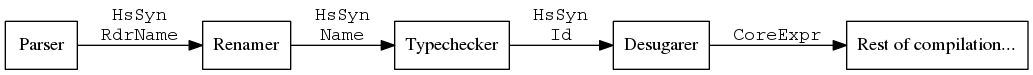
\includegraphics[scale=.4]{graphVis/Chapter2/compilerStgs.png}
	\end{center}
	\caption{GHC Compiler stages.}
	\label{compilerStages}
\end{figure}

Some of the major components and the order in which they are used in GHC are shown in Figure~\ref{compilerStages} which has been adapted from~\citep{ghcDesign}. This figure is not a complete list of all the components GHC uses, just the parts that HaRe interacts with. The full diagram can be found in~\citep{ghcDesign}. The label after each compiler stage indicates the type of AST that is produced by that stage.

The top level data type for all of the GHC abstract syntax is \texttt{HsSyn} ~\citep{ghcDesign}. \texttt{HsSyn} is parameterised by some identifier type; each compiler stage produces a different type of identifier with the additional information that stage produces. For example the typechecker takes in an AST parameterised by \texttt{Name} and returns an AST parameterised by \texttt{Id} which is a \texttt{Name} with additional type information.

\subsection{GHC's Name Types}\label{ghcNames}

There are five name types that GHC uses, they are:

\begin{itemize}
	\item \texttt{OccName} is the simplest type of name. It is just a wrapper around a \texttt{FastString}, which is an array of bytes, and an optional \texttt{NameSpace}. An \texttt{OccName} is contained in each of the other four identifier types.
	\item \texttt{RdrName} names are produced by GHC's parser. \texttt{RdrName}s are essentially just an \texttt{OccName} with optional module information if the source name has been qualified. 
	\item \texttt{Name}s are produced by the renamer. A \texttt{Name} contains an \texttt{OccName} and a \texttt{Unique} that differentiates \texttt{Name}s that have the same \texttt{OccName}. A \texttt{Unique} is just an integer but it is generated by the GHC in such a way so that it is guaranteed to be unique. They have also had their scoping and binding resolved, so each \texttt{Name} contains the source span where that name was defined and a data type that describes what type of \texttt{Name} it is (e.g. a name defined internally in the module or a name from another module).
	\item \texttt{Id} \& \texttt{Var} are the identifiers produced by the typechecker.\footnote{\texttt{Id} is just a synonym for \texttt{Var}.} These identifiers contain a \texttt{Name}, and a \texttt{Unique}. Finally these names also contain the type of the variable they represent. 
\end{itemize}

These identifier types change throughout the compilation process but these names only parameterise the syntax tree, the shape of the tree itself stays the same throughout compilation. 

\subsection{GHC's syntax tree}
GHC's abstract syntax is currently made up of over 90 data types. Many of those types have multiple constructors; the expression data type \texttt{HsExpr} for example has over 40 constructors. This section will briefly introduce the structure of GHC's abstract syntax tree.

\subsubsection{Common syntax types}

The most common type in any given piece of GHC abstract syntax would be a \texttt{Located} as seen in Figure~\ref{located}.

\begin{figure}[t]
\begin{lstlisting}

type Located e = GenLocated SrcSpan e

\end{lstlisting}
\caption{The \texttt{located} type.}
\label{located}
\end{figure}

\texttt{Located} is used to tag syntax elements with their position in a source file. The \texttt{SrcSpan} contains the filename that the span comes from and then the start and end columns and start and end lines that the span covers.\footnote{GHC has small optimisation where if a span exists entirely on a single line it only stores the single line number and the start and end column, instead of storing the same line number twice.} 

There are located versions of many of the AST types. For example, \texttt{HsExpr} is the type that represents expressions, and there is a related type \texttt{LHsExpr} that represents a located expression whose definition is shown in Figure~\ref{lhsexpr}.

\begin{figure}[t]
\begin{lstlisting}
type LHsExpr id = Located (HsExpr id)
\end{lstlisting}
\caption{The located expression}
\label{lhsexpr}
\end{figure}

The \texttt{HsExpr} type represents much of the Haskell language such as function application, lambdas, if and case statements. Pattern matching is handled by a \texttt{MatchGroup} type. Each \texttt{MatchGroup} contains a list of \texttt{Match}es and some typing information. Consider the case statement in Figure~\ref{caseStmt}.

\begin{figure}[t]
\begin{lstlisting}
case (x, y) of
	(Just i, Just j) -> Just (i+j)	
	(Just _, Nothing) -> x
	(Nothing, Just _) -> y
	(Nothing, Nothing) -> Nothing
\end{lstlisting}
\caption{A case statement}
\label{caseStmt}
\end{figure}

This would be parsed into the \texttt{HsCase} constructor of \texttt{HsExpr}. This constructor is seen in Figure~\ref{hscase}. The first constructor argument represents the expression that the patterns are matched against (the tuple \texttt{(x,y)} in this case). The abstract syntax tree of this expression is shown in Figure~\ref{caseAST}. The second argument to \texttt{HsCase} represents all four of the matches in the case statement. \texttt{MatchGroup}s are used to represent any code that associates some patterns with a right hand side expression. Function bindings, lambda expression, and case statements all use \texttt{MatchGroup}s. 

\begin{figure}[t]
\begin{lstlisting}
HsCase (LHsExpr id) (MatchGroup id (LHsExpr id))	
\end{lstlisting}
\caption{The \texttt{HsCase} constructor}
\label{hscase}
\end{figure}

\begin{figure}[t]
\begin{lstlisting}
(L {case.hs:(3,11)-(7,31)} 
                 (HsCase 
                  (L {case.hs:3:16-21} 
                   (ExplicitTuple 
                    [
                     (L {case.hs:3:17} 
                      (Present 
                       (L {case.hs:3:17} 
                        (HsVar 
                         (Unqual {OccName: x}))))),
                     (L {case.hs:3:20} 
                      (Present 
                       (L {case.hs:3:20} 
                        (HsVar 
                         (Unqual {OccName: y})))))]))
\end{lstlisting}
\caption{The fragment of parsed abstract syntax representing the expression being pattern matched in Figure~\ref{caseStmt}.}
\label{caseAST}
\end{figure}

In the case expression from Figure~\ref{caseStmt} each of the four pattern matches is a \texttt{Match} in the expressions \texttt{MatchGroup}. Each \texttt{Match} associates a left hand side pattern with the appropriate right hand side expression. 

\subsubsection{The syntax tree}
The previous section gave a brief overview of GHC's identifiers and its representation of expressions. This section describes the broader picture, the representation of whole Haskell programs.  

According to the GHC a Haskell program is simply a list of modules.\footnote{This is a very simple view and additional tools are needed to properly represent "projects" which is the context that most Haskell programs exist inside of. This is discussed further in Section~\ref{hareInners}.} Inside of GHC each module is represented by an \texttt{HsModule}. This top level structure keeps track of everything that the module imports, exports, and a list of all the declarations that the module defines. Declarations (of type \texttt{HsDecl}) are what represent everything that can be defined in Haskell. 

The \texttt{HsDecl} type is only used as a wrapper around other types. Bindings (of functions and/or values), instance, and type class declaration are differentiated by \texttt{HsDecl}'s constructors. A few of the more common \texttt{HsDecl} constructors are shown in Figure~\ref{hsdecl}. 

\begin{figure}
\begin{lstlisting}
data HsDecl id =
	   TyClD (TyClDecl id)
	| InstD (InstDecl id)
	| ValD  (HsBind id)
\end{lstlisting}
\caption{A subset of \texttt{HsDecl constructors}}
\label{hsdecl}
\end{figure}

\texttt{HsDecl} only provides a high level categorisation of what type it is. There is very little information stored at this level, the inner type is the "payload" of the declaration (e.g. \texttt{HsBind} or \texttt{TyClDecl}). These payload types are what store the type and expression level abstract syntax of Haskell that was described in the previous section.

Some notable payload types are \texttt{TyClDecl}, \texttt{InstDecl}, \texttt{HsBind}, and \texttt{Sig}. \texttt{TyClDecl} represents a family, type synonym, data, or type class declaration. The \texttt{InstDecl} is used to represent the instance declarations for type classes, and data or type families. The real workhorse of the language is \texttt{HsBind}. \texttt{HsBind} represents functions and pattern bindings (e.g. \texttt{(x,y) = (1,2)}). The \texttt{HsBind} type also has constructors that are introduced by the type checker such as dictionary binding. Finally \texttt{Sig} is the data type that represents type signatures. 

\section{Generic programming}
\label{genProg}

The need for a generic programming library, as previously discussed in Section~\ref{prog&Strafunski}, remains the same when using the GHC API's AST as opposed to Programatica's. Currently HaRe still uses Strafunski-StrategyLib as well as another library, Scrap Your Boilerplate. Scrap Your Boilerplate (SYB) is a generic programming library developed by Ralf L{\"a}mmel and Simon Peyton-Jones~\citep{syb}. 

SYB is included with GHC and has become the Haskell community's standard generic traversal library, however HaRe still uses Strafunski because it provides ``stop'' traversals. These traversals (stop-top-down, type preserving, and type unifying) descend the tree until the strategy ``succeeds'' (that is, the extended function can be applied) and then stops. Essentially it cuts a line across the abstract syntax tree where everything below the line is unvisited. This traversal is useful when refactoring because of how the ASTs types are nested within each other. For example, a refactoring commonly wants to modify the body of a function and the stop traversals ensure that when the extended function is applied, it is applied with the expression representing the whole binding rather than sub-expressions.

\subsection{Generic Traversals}
The Stratego/XT library was one of first systems for programming tree transformations in a systematic way~\citep{stratego}. Stratego developed the idea of a transformation strategy. A strategy is the combination of a term rewriting function and a traversal function that describes how that rewriting function should be applied to a tree of terms. Stratego provides combinators that help construct term rewriting functions and tree traversal functions \citep{stratego}.

Stratego is an untyped transformation system and so was unsuitable for working with the statically typed Haskell. Strafunski was ``largely inspired'' by Stratego, but for a statically typed context~\citep{strafunski}.
  
\subsection{Scrap Your Boilerplate}\label{syb}

	Scrap Your Boilerplate (SYB) is a generic traversal library for Haskell that was inspired by Strafunski~\citep{syb}. SYB comes with GHC and has become the most used generic programming library in the Haskell community.\footnote{According to \url{http://packdeps.haskellers.com/reverse}} 

	Suppose there was a simple expression language that contained integers, integer addition, assignment, and variables. This language is represented by the type defined in Figure~\ref{expression} and a function that works over this type to rename a variable "x" to "a" is defined in Figure~\ref{renamexvar}.
	
	\begin{figure}[t]
	\begin{lstlisting}
type Name = String

data Expr =
     Value Int
   | Var Name
   | Add Expr Expr
   | Assign Name Expr
      deriving(Data,Typeable)
	\end{lstlisting}
	\caption{A simple expression type.}
	\label{expression}
	\end{figure}
	
	\begin{figure}[t]
	\begin{lstlisting}
renameXVar :: Expr -> Expr
renameXVar (Var "x") = Var "a"
renameXVar (Assign c e) = 
	| c == "x" = Assign "a" (renameXVar e)
	| otherwise = Assign c (renameXVar e)
renameXVar (Add e1 e2) = Add (renameXVar e1) (renameXVar e2)
renameXVar v = v
	\end{lstlisting}
	\caption{A function to rename the "x" variable.}
	\label{renamexvar}
	\end{figure}
	
	There are four cases to the \texttt{renameXVar} function. The first case matches when \texttt{renameXVar} is called with a \texttt{(Var "x")} value. This is one of the cases that the function will replace the "x" name with an "a" name. The second case matches an assignment and is the other case when actual ``work'' happens. In this case the function needs to check if the variable being assigned is an "x" or not, if it is then the name being assigned is replaced with "a" otherwise the name remains the same. Then there is a recursive call replace the name in the right hand side of the assignment. The other two cases will not directly modify an expression. In the \texttt{Add} case there is just a recursive call to perform replacements in its sub-expressions. The final case is just a catch-all term that returns its parameter. This will be called when \texttt{renameXVar} is called with a \texttt{Value} or a \texttt{Var} that is not \texttt{"x"}.
	
	This is fairly straightforward and doesn't take much time to write. However, if subtraction was added to the definition of expression \texttt{renameXVar} would need to be updated as well to include a recursive call very similar to the addition case. These duplicated recursive calls are  just boilerplate code~\citep{syb}. In this small example having a few of these types of cases is not an issue. However, as the expression begins to approach the size of an actual programming language writing traversals like \texttt{renameXVar} would become much more time-consuming and a nightmare to maintain. 
	
	The reduction of boilerplate code like this is the point of SYB. SYB allows us to rewrite \texttt{renameXVar} as shown in Figure~\ref{renameSYB}.
	
	\begin{figure}[t]
	\begin{lstlisting}
import Data.Generics	
	
rename :: Name -> Name
rename "x" = "a"
rename n = n

renameXVar :: Expr -> Expr
renameXVar = everywhere (mkT rename)
\end{lstlisting}
\caption{\texttt{renameXVar} written using SYB}
\label{renameSYB}
\end{figure} 
	
This example nicely illustrates the four key components of an SYB traversal~\citep{syb}.

	\begin{itemize}
		\item The function that performs the "interesting" part of the traversal
		\item A type extension for that function
		\item A generic traversal combinator
		\item The data type to be traversed must be an instance of the \texttt{Typeable} and \texttt{Data} classes (as explained below)
	\end{itemize}
	
	From the example mentioned previously the "interesting" part of this traversal is the rename function, because this function contains the code that actually changes the name "x" to the name "a." The \texttt{mkT} function extends the type of the \texttt{rename} function to \texttt{Typeable~a = > a~ -> a}. 
	
	Type extension allows for the \texttt{rename} function to work over any members of the \texttt{Typeable} class rather than just \texttt{Name}s. The extended version of \texttt{rename} will work as expected when provided with an argument of type \texttt{Name}, and if an argument of any other type is provided the traversal will continue onto the argument's component parts if it has any and returns the argument unchanged otherwise.
	
	The \texttt{everywhere} function is this traversal's generic combinator. \texttt{everywhere} can apply a generic function to every node in a tree in a bottom-up manner, as long as that tree is of type \texttt{Data} and \texttt{Typeable}. A member of the \texttt{Typeable} class has defined a generic representation of itself and members of the \texttt{Data} class implement generic folding operations.	As you can see that the \texttt{Expr} data type, from Figure~\ref{expression}, derives both the \texttt{Typeable} and \texttt{Data} classes so it can be traversed by \texttt{everywhere}.  
	
\subsubsection{Types of Generic Algorithms}

SYB defines three types of generic algorithms: transformations, queries, and monadic transformations. The \texttt{rename} example from the previous section is an example of a transformation. Transformations preserve the type of the structure that is traversed. Queries, on the other hand, are "type unifying" algorithms. Queries are good for summarizing information contained in a data structure. You would use a query, for example, to traverse an expression and collect all of its bound variables. Using the same expression type (Figure~\ref{expression}) from the previous section, the following function extracts all bound variables from a given expression.

\begin{figure}[t]
\begin{lstlisting}
bVars :: Expr -> [Name]
bVars e = everything (++) ([] `mkQ` f) e
	where f (Assign nm _) = [nm]
          f _             = []
\end{lstlisting}
\caption{A generic function that collects all bound variables from an expression.}
\end{figure}

\texttt{everything}, as seen in the \texttt{bVars} function from the previous listing, is the generic query combinator that summarises all nodes, top down from left to right~\citep{sybDocs}. The first argument to \texttt{everything} is the function it uses to combine separate results from the query. In this case, all the lists of names will be appended together. The "interesting" function \texttt{f} that actually returns a \texttt{Name} when one is being bound is extended via the \texttt{mkQ} function. \texttt{mkQ} will apply \texttt{f} when possible otherwise it will just return the empty list.

It is also useful to do transformations from within some monadic context. A simple example of this would be to rewrite the finding bound variables example from previously but instead the list of found results is stored as a piece of state.

\begin{figure}[t]
\begin{lstlisting}
type TransformState = State [Name]

bVars :: Expr -> [Name]
bVars e = execState findVars []
  where findVars = everywhereM (mkM f) e
        f :: Expr -> TransformState Expr
        f e@(Assign n _ ) = do
          modify (\lst -> n:lst)
          return e
        f e = return e
\end{lstlisting}
\caption{Finding bound variables using the state monad}
\end{figure}

A big advantage of monadic traversals is that both querying and transformations can happen in a single pass. The example in Figure~\ref{renameVars} renames every \texttt{Name} in an expression by adding \texttt{"\_old"} as a suffix and stores the original names in a list. 

\begin{figure}[t]
\begin{lstlisting}
renameVars :: Expr -> TransformState Expr
renameVars e = everywhereM (mkM f) e
  where f :: Expr -> TransformState Expr
          f (Assign n e) = do
            modify (\lst -> n:lst)
            return (Assign (n++"_old") e)
          f (Var n) = return (Var (n++"_old"))
          f e = return e
\end{lstlisting}
\caption{Changing every found name and storing the old names in a list.}
\label{renameVars}
\end{figure}
 
This type of generic traversal is very common in HaRe because traversals often need to make use of a refactoring's stored state or run something from the GHC API which needs the features provided by an instance of \texttt{GhcMonad}, all while modifying the abstract syntax. The GHC API's operations all work within the \texttt{GhcMonad} that provides the features GHC needs to compile a single Haskell source file such as IO, logging warning, exception handling, and keeping track of the compilation session~\citep{ghcApi}.   
	 
\section{ghc-exactprint}
\label{ghcExactprint}

After using generic programming to transform the abstract syntax, HaRe needs to be able to print the modified code. A challenging part of building a refactoring tool is that a user will not want non-refactored parts of their code to change at all. HaRe needs to preserve the user's comments and spacing from the source file.

Prior to GHC version 7.10.1, the location of certain keywords and punctuation (such as \texttt{do} and \texttt{let}) and user comments were lost after parsing. This made parsing and then printing an exact copy of a GHC Haskell source file impossible if you only had a copy of its AST. GHC's 7.10.1 release added annotations for the "lost" syntax elements that had previously not been represented in the parsed abstract syntax~\citep{apiAnns}. 

The parsed source now includes a map that associates each ``lost'' keyword with the source span that the keyword can be found in, and that keyword's exact location. This approach was taken to avoid littering the existing AST with functionally meaningless keyword data~\citep{apiAnns}. 

Even with the position of every syntax element being recorded, printing a module after the AST has been modified is not easy. Many AST elements are "located" with a source span that indicates that element's exact position in the file. This means that any change to the AST will require updating the location of all the syntax elements that occur later in the line at least for single line changes and, in the case of changes that modify entire lines, every element after that change will need its location to be updated.

Ghc-exactprint simplifies this immensely by allowing us to position elements relative to their neighbours rather than absolutely~\citep{exactprint}. After parsing a source file, HaRe takes the annotations GHC returns with the parsed abstract syntax and relativises them using ghc-exactprint. For each syntax element ghc-exactprint creates a new data type called an "\texttt{Annotation}" which contains an offset that indicates where this element should be positioned compared to the previous element. Take for example the definition in Figure~\ref{strangeSpacing}.

\begin{figure}[t]
\begin{lstlisting} 
f a = (a+ 1 )
\end{lstlisting}
\caption{A definition with strange spacing.}
\label{strangeSpacing}
\end{figure}


The absolute position of the plus sign is row one column nine (GHC's locations are one-based) but using ghc-exactprint we instead can think of the position of the plus sign using the offset \texttt{(0,0)} because there is no space between it and the previous element (the variable \texttt{a}). Using this system the number literal following the plus sign has an offset of (0,1) because of the single column of space before it. 

The \texttt{Annotation}s are stored in a map that is keyed based on the parsed location of a syntax element and the string representation of the AST constructor. In the previous example the right hand side of the definition is located at the source span (1,7)-(1,13) which stands for ``row one columns seven through thirteen'' and GHC represents this expression with the \texttt{HsPar} constructor for the \texttt{HsExpr} type. The source span and the constructor together can be combined to retrieve the annotation data associated with this fragment of the AST. This syntax tree has two elements associated with it, the opening and closing parenthesis. Each of these keywords is given its own offset, which in this case is (0,0) for the opening parenthesis\footnote{The offset in this case is (0,0) and not (0,1) as you might expect because the space between the equals sign and the opening parenthesis is represented in the offset for the entire right hand side expression.} and (0,1) for the closing parentheses. We could obviously infer from the use of the \texttt{HsPar} constructor that this tree is wrapped in parentheses however the user's specific spacing would be lost without the annotations.

Comments are another element of a source file that prior to GHC 7.10.1 were "lost" after parsing. Using ghc-exactprint comments are stored in the annotations associated with the next piece of syntax. In the code snippet in Figure~\ref{commentSnippet} the comment on line three is added to the annotations associated with the declaration of the function \texttt{f} along with a delta position that indicates the comment is a single line before this declaration starts.

\begin{figure}[t]
\begin{lstlisting}
type Name = String

--a comment
f i = i + 1
\end{lstlisting}
\caption{The comment is ``attached'' to the AST of the function \texttt{f}.}
\label{commentSnippet}
\end{figure}




\section{The current implementation of HaRe}
\label{hareCurr}

\begin{figure}[t]
	\begin{center}
		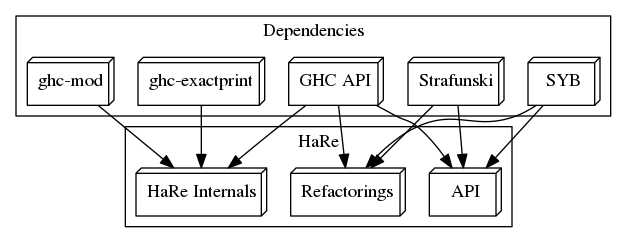
\includegraphics[scale=.4]{graphVis/Chapter2/hareDesign.png}
	\end{center}
	\caption{A diagram of the components of HaRe and their dependencies.}
	\label{design}
\end{figure}

We have just discussed the major components that HaRe depends on. The ghc-api gives us access to the internal representation of Haskell, the generic programming libraries Scrap Your Boilerplate and Strafunski-StrategyLib allow HaRe to work more easily with that internal representation, and ghc-exactprint is how HaRe preserves the source files spacing when writing the output file. The relationship between the dependencies and HaRe's components is shown in Figure~\ref{design}. From this foundation we can make HaRe focused on refactoring rather than solving these more generic problems. This section will discuss how HaRe is implemented, what its API provides, and some general conventions that its refactorings use.

\subsection{The Internal Structure of HaRe}
\label{hareInners}

The GHC API exposes all the functionality needed to compile a set of Haskell source files. In reality Haskell programs consist of more than just single source files without dependencies. Projects are organised using build tools such as Cabal~\citep{cabal} or Stack~\citep{stack} that handle these issues for the programmer. HaRe needs to be aware of the context that these tools provide because refactorings may change multiple modules or modify modules that import modules from external dependencies. In HaRe's case, ghc-mod provides a monadic context that handles these build environments and compiler setup~\citep{ghcMod}. Within ghc-mod's context, HaRe keeps track of the state of the refactoring session.

\begin{figure}[t]
\begin{lstlisting}
newtype RefactGhc a = RefactGhc
    { unRefactGhc :: GM.GhcModT (StateT RefactState IO) a}
\end{lstlisting}
\caption{HaRe's Monad \texttt{RefactGhc}}
\label{refactghc}
\end{figure}

Figure~\ref{refactghc} shows the definition of HaRe's monad that each refactoring runs in. \texttt{RefactState} is an algebraic data type that keeps track of all the settings, abstract syntax, and filepath for refactoring a single file. It is possible to refactor client modules by setting the filepath in the \texttt{RefactState} to target another module. HaRe will then parse and typecheck that module's information into the state for transformation.

Even though there are three types of the AST, the annotations are only included in the parsed AST. Once a refactoring has finished, all of its changes need to be reflected in the parsed abstract syntax tree and its annotations because this is the structure that ghc-exactprint works over. HaRe's state still contains all three of the syntax trees because the renamed and typed sources are useful for the additional type and scope information they contain about a source file. 

\subsection{HaRe's API}

Modifying and reasoning about GHC's abstract syntax and maintaining the associated annotations is still a complex task, even with help from HaRe's dependencies. HaRe defines its own API to help fill this gap between its dependencies and its refactorings. In addition to the obvious functions that are required for running a refactoring within the \texttt{RefactGhc} monad, the API also includes helper functions that make working with the state easier. 

HaRe also defines a large collection of program analysis and transformation functions. For example, pulling the binding of a top level variable from a module's entire abstract syntax tree is a task that many refactorings have to do so this functionality is part of HaRe's API. There are also small program transformations that are not in and of themselves refactorings but common low level modifications that are useful to several refactorings, such as adding a new import declaration or making a function infix by wrapping it in back quotes (the \texttt{`} character).

Additionally there are several transformations that don't affect the abstract syntax as much as they change the annotations that format ghc-exactprint's output. Adding new lines before a syntax element doesn't change the meaning of a program but is important for a refactoring's output to be well formatted and easy to read. 

HaRe's dependencies help abstract away the low-level\footnote{Low level from the perspective of a refactoring at least.} details of a language back-end, build tools, and pretty printing. HaRe's API tries to close the gap still left between the dependencies and the refactorings themselves. In the next section we will take a look at how HaRe's refactorings are implemented.


\subsection{Implementing Refactorings in HaRe}

HaRe actually requires very few things from a refactoring implementation. As was mentioned previously in Section~\ref{hareInners}, everything must run inside the \texttt{RefactGhc} monad whose state is where the abstract syntax of a target module is stored. A refactoring is also expected to return a list of  "\texttt{ApplyRefacResult}s" which contains an updated parsed AST and annotations along with the filepath the AST originated from; this updated AST is what HaRe writes out as the result of the refactoring\footnote{HaRe actually outputs to a temporary file. When refactoring "file.hs" HaRe produces "file.refactored.hs." This allows programmers to check the result of a refactoring before overwriting the existing module.}  

Beyond those two features, refactorings are free to be implemented however the programmer chooses. However, certain conventions have been adopted within many of HaRe's refactorings. When describing a refactoring one would imagine that checking \textit{pre}conditions would be the first thing the implementation of that refactoring computes. A more efficient implementation checks preconditions throughout computation alongside the AST transformation. For example, the renaming refactoring doesn't check for name clashes in client modules until after the source module has been modified. If a name clash is found in a client module then an error is thrown at that point and the whole refactoring is rolled back. Though this slows down the time to failure somewhat, it saves HaRe from traversing every client module twice, once for preconditions and a second time for rewriting.

Merging precondition checking with transformation saves the refactoring from traversing parts of the AST multiple times. For example, the renaming refactoring checks for name conflicts while it descends the AST, replacing the old name with the new one. Obviously this strategy only works for certain preconditions: the only precondition for deleting a definition is that the target definition is not used. The transformation only affects the syntax tree of the definition to be deleted so the implementation of the refactoring has to do a separate scan of the rest of the target module and any of its client modules to determine if the target definition is used or not.

\subsection{Using the GHC's Abstract Syntax Trees}
Each stage of the compiler takes the previous stage's output and creates it's own version of the tree decorated with some additional information. This provides a challenge when writing refactorings because all of the changes made to the source needs to be reflected in the parsed syntax tree. The additional name and type information can be retrieved from the other trees but they will have to be traversed from the top down to where the refactoring is taking place.

In the same way that the a refactoring can be sped up through careful consideration of how much re-traversing of the abstract syntax tree is absolutely necessary, it is also important to be mindful of when it is absolutely necessary to traverse through the other stages' trees. For the most part HaRe's refactorings can avoid having to look up information in either the renamed or typechecked trees. The renaming refactoring, for example, uses a \texttt{NameMap} which associates every \texttt{RdrName} in the parsed source with it's \texttt{Name} from the renamed source. This allows the refactoring to ensure that the instance of a variable it is going to rename is actually the targeted variable and not just a variable with the same name in a different scope. This map is calculated at the start of the refactoring, so the renamed syntax tree only needs to be completely traversed once rather than over and over again to check if each name that matches the target variable's name.

Collecting any required information from the other syntax trees, up front, is a good way to limit the amount that these trees are traversed, but often traversing these trees can be entirely avoided. For example, the generalising \texttt{Maybe} refactoring described in Chapter~\ref{chp:ddRefs} works on replacing the \texttt{Maybe} type with a more generic type if possible. \texttt{Maybe a} is a type that represents a computation that may return a value of type \texttt{a} or fail in some way, this case is represented by a \texttt{Nothing} constructor. This generalising \texttt{Maybe} refactoring, rather than checking the type of all the \texttt{Just}s and \texttt{Nothing}s encountered in the target program to make sure that they are actually of type \texttt{Maybe}, instead the refactoring begins by checking the imports of the target module to see if the \texttt{Data.Maybe} module has been given a qualification and takes into account that the target module will refer to the \texttt{Maybe} type with a non-standard name. After that check, since \texttt{Maybe} is included in the prelude it is safe to assume that any \texttt{Just}s and \texttt{Nothing}s in the target program are of type maybe.

One refactoring that does need to reference the typed syntax tree fairly heavily is the List to Hughes List refactoring described in Section~\ref{listToDlist}. This refactoring needs to change the type of entire subtrees, so it references the typed syntax tree to see what the type of the current node is during the transformation. This is fairly straightforward due to the source being tagged with \texttt{SrcSpan}s that are consistent throughout the compilation process. This means that a piece of typed abstract syntax is the same as a particular parsed syntax subtree if their \texttt{SrcSpan}s are the same. Searching through the later compilation stage's trees is as simple as doing a full traversal of the tree searching for the appropriate \texttt{SrcSpan}. 

In general most of the time the parsed syntax contains enough information to perform a refactoring. Since the parsed AST is also where changes must be made for ghc-exactprint to output the modifications most of the refactorings only look at the parsed AST. If information is required from one of the other compilation stages it is either pre-collected at the start of the refactoring, or the \texttt{SrcSpan}s that decorate all of the syntax trees can be used to navigate to the equivalent points in different syntax trees.



\subsection{The Development Process of HaRe}

Very little, if any, of the code from the original implementation of HaRe is used today. Development of HaRe has been coordinated through GitHub\footnote{\url{https://github.com/RefactoringTools/HaRe}} since 2011. When I began working on HaRe in 2013, Alan Zimmerman had upgraded much of the internal structure of HaRe to use the GHC API. 

The internal structure of HaRe is mostly the work of Alan, however a description of the current implementation has not appeared in the literature yet and so it has been described in some detail here. My contributions to HaRe are in the development of the refactorings described throughout this thesis and in the creation of a high level API for program analysis, synthesis, and transformation which is described in Section~\ref{hareAPI}.



\chapter{Data-driven refactorings}
\label{chp:ddRefs}

Some refactorings focus on rewriting the structure of a program (e.g. refactoring an \texttt{if} to \texttt{case} statement), but a data-driven refactoring focuses on the types that a program works over and \textit{how} that program manipulates those types. Any changes that a data-driven refactoring makes to the structure of the program are \textit{driven} by the data types of that program rather than being the main motivation of performing the refactoring. 

Consider the introducing a type synonym refactoring that is described in Section~\ref{introSyn}, this refactoring adds a type synonym for some type. The motivation behind this is keeping the types of your program up to date with what they are meant to represent. For example, if some strings are used to represent customer names in a program, introducing a synonym for strings called \texttt{Name} helps clarify what data certain strings are supposed to represent. In this way the refactoring's changes to the source program are motivated by the data in that program and the desire for the program's types to better communicate the nature of that data.

This chapter begins with a discussion of data-driven refactorings for imperative object-oriented languages in Section~\ref{ooRefs}. Imperative programs are written as a sequence of steps that modify an object to the desired output state. Types in an object-oriented program also exist in a strict hierarchy. These two factors mean that object-oriented data-driven refactorings modify the hierarchy while leaving the structure of the code mostly intact. The rest of this chapter will describe data-driven refactorings for functional programs.

In comparison to the imperative way of constructing programs, functional programs describe the relationship between the input and output data. Functional programming languages also tend to offer a much richer type system than object-oriented languages where data types are typically either objects or a non-user expandable set of primitive types. These two facts mean that the structure of a functional program can be determined by the types it works over to a much greater degree than in imperative languages. 

Section~\ref{introSyn} describes the ``introducing a type synonym'' refactoring. This is the renaming of data-driven refactorings: neither the structure nor the type of the target program changes, just how the program refers to the types it works over. Next, Section~\ref{genMaybe} describes a generalisation refactoring. This thesis outlines two generalisations, one (described in Section~\ref{genMaybe}) makes code of a specific type (\texttt{Maybe}) work over a type class (\texttt{MonadPlus} or \texttt{Monad}) instead. The other generalises code of one type class to use a class higher the hierarchy (covered in Chapter~\ref{chp:applicative}). Finally Section~\ref{listToDlist} describes a refactoring that tranforms programs that work over lists to instead use an alternate implementation of lists. The refactoring method described in this chapter could be applied to refactor between any types that can be projected onto another type.

\section{Object-Oriented Data Refactorings}\label{ooRefs}

The origins of refactoring are deeply rooted in the object-oriented world~(\cite{programRestructuring};~\cite{refactOOFrameworks}), though Though it traces its origins to work on transforming Algol~\citep{recursiveTransformation}. The canonical catalogue of refactorings remains Martin Fowler's \emph{Refactoring: Improving the Design of Existing Code} ~\citep{fowler}. Fowler's catalogue of refactorings are all written in Java though he purposefully avoided using any features that were unique to Java, so that the refactorings could be applicable in many different programming languages.

As a functional programmer when going through this catalogue of refactorings there seem to be three types of refactorings.

\begin{itemize}
	\item Refactorings that are directly applicable in a functional language
	\item Refactorings that could be adapted for use in a functional language
	\item Refactorings not applicable to a functional language
\end{itemize}

That first type of refactorings are structural refactorings and their usefulness to a functional program is easily understood. Refactorings like renaming or adding a parameter don't depend on object-oriented features existing in the target language.

The third type of refactorings are so dependent on features associated with object-oriented languages that they are impossible to implement or have no equivalent in a functional language. The "remove setting method" refactoring depends on the common OO pattern of each field of a class having "getter" and "setter" methods that retrieve or modify that field respectively. This pattern, on the other hand, is not as ubiquitous in functional languages because most do not support objects, and immutability makes a "setter" function irrelevant. OCaml would be a notable exception to this rule: OCaml supports objects and allows the programmer to mark variables as mutable, and so getter and setter methods are possible.

\begin{figure}[t]
\begin{lstlisting}[language=caml, morekeywords={object,method}]
let mInt init_i = object
    val mutable i = init_i

    method get_i = i
    method set_i new_i =
      i <- new_i
  end
\end{lstlisting}
\caption{An OCaml object with getter and setter methods.}
\label{ocamlObj}
\end{figure}

The OCaml object from Figure~\ref{ocamlObj} would be a valid target for this refactoring. However these methods are not as common as they are in imperative object-oriented languages with mutable data as the default, so a refactoring to remove a setter method is of limited value even for OCaml.

The second type of refactoring found in~\citep{fowler} is much more interesting to a functional programmer. The specifics of these refactorings are not directly applicable to functional programs but the underlying motivations are relevant to any programming paradigm. 

For example here is the motivation for the "Replace Data Value with Object" refactoring in~\citep[pg. 175]{fowler}:

\begin{displayquote}
Often in early stages of development you make decisions about representing simple facts as simple data items. As development proceeds you realize that those simple items aren't so simple anymore. A telephone number may be represented as a string for a while, but later you realize that the telephone needs special behavior for formatting, extracting the area code, and the like. For one or two items you may put methods in the owning object, but quickly the code smells of duplication and feature envy\footnote{Feature envy is when the methods of a class are more interesting in a different object than the one it is in.}. When the smell begins, turn the data value into an object.
\end{displayquote}

This refactoring extracts a field that was some primitive type into an object. The example from~\citep{fowler} works over an order class with a string that represents the customer that placed an order.

\begin{figure}[t]
\begin{lstlisting}[language = java,tabsize=4]
class Order {
	public Order (String customer) {
		_customer = customer;	
	}
	
	public String getCustomer() {
		return _customer;
	}
	
	public void setCustomer(String arg){
		_customer = arg;	
	}
	
	private String _customer;
}
\end{lstlisting}
\caption{The Order class}
\end{figure}

The refactoring creates a new customer class that has a string field with a getter method as seen in Figure~\ref{custCls}. The customer class doesn't add any additional features but the extra layer of abstraction sets up the code base for further development. The customer object could have fields added that represent contact info or further demographic information without polluting the order class with order-irrelevant data.

\begin{figure}[t]
\begin{lstlisting}[language = java,tabsize=4]
class Order {
	public Order (String customer) {
		_customer = new Customer(customer);	
	}
	
	public String getCustomer() {
		return _customer.getName();
	}
	
	public void setCustomer(String arg){
		_customer = new Customer(arg);	
	}
	
	private Customer _customer;
}

class Customer {
	public Customer(String name){
		_name = name;
	}
	
	public String getName() {
		return _name;
	}
	
	private final String _name;
}
\end{lstlisting}
\caption{The result of the Replace Data Value with Object refactoring when applied to the customer field of the order class.}
\label{custCls}
\end{figure}

Functional programmers have to make similar data representation decisions as the object-oriented programmer. At the start of a project representing a customer just by their name could be reasonable. As the project develops this can become a serious limitation and a more robust abstraction is required. 

This section introduced how object-oriented refactorings help build up the data model over the lifetime of a project. These sorts of refactorings for a language with a rich type system like Haskell offer many more choices for evolving the data model of a system. Though a Haskell programmer can take inspiration or directly reimplement several of the canonical Fowler refactorings there may be additional refactorings that are completely functional with no OO counterparts. The rest of this chapter will describe refactorings for Haskell that support data model evolution.  

%\begin{figure}[t]
%\begin{lstlisting}
%data Customer = Customer {name :: String}
%\end{lstlisting}
%\caption{The algebraic data type for \texttt{Customer}.}
%\label{custData}
%\end{figure}
\section{Data-Driven Refactorings in Haskell}

Haskell offers a rich environment for data representation. The Haskell 2010 standard defines several types that are included in the prelude, including tuples, lists, characters, strings (which are just lists of characters), several types of numbers, and the function type. Additionally, programmers can construct new types with algebraic and abstract data types or rename existing types with type synonyms. Type classes support overloading as well. The standard library of GHC comes with many type classes that can help produce powerful abstractions~\citep{typeclassopedia}. Contrast this with how most object-oriented type systems are either unified, where every type is a subclass of some top level \texttt{Object} class, (e.g. C\# or Ruby) or there are a fixed set of predefined primitive types as well as the object hierarchy (e.g. C++ and Java's type systems). 

These two different approaches to type systems both have pros and cons, which have sparked a vigorous (and quite possibly eternal) debate. The goal of this thesis is not to add to this debate, instead it is to build from a number of general principles that transcend the debate.

\begin{itemize}
	\item Data representation is a language independent problem that must be answered in every project.
	\item The way a project manages and represents its data is very likely to evolve over a project's lifetime and this is indeed desirable.
	\item Refactoring is a structured way to support this evolution.
		\item Refactorings for a language like Haskell need to take a different approach than those for object-oriented languages, particularly when refactorings are data-driven rather than ``structural.''  
	\item Data representation in a rich type system like Haskell's, in some sense, determines the structure of the program.
\end{itemize} 

\subsection{Introducing a Type Synonym}\label{introSyn}

Type synonyms in Haskell, as mentioned previously, are a way to name an existing type. A simple example can be seen in Figure~\ref{fooSyn}. 

\begin{figure}[t]
	\begin{lstlisting}
type Foo = (String, Int)

f :: Foo -> Foo
f x@(_, 0) = x
f (str, i) = (tail str, i-1) 
	\end{lstlisting}
	\caption{A simple type synonym.}\label{fooSyn}
\end{figure}

Any place that where the \texttt{Foo} synonym is in scope the new name can be used to refer to any value of type \texttt{(String, Int)}. In fact "\texttt{Foo}s" and "\texttt{(String, Int)}s" are completely interchangeable. Introducing a synonym is a good way to quickly and simply name types to suggest their specific use in the current application.

Returning to the example from~\citep{fowler} of an order type that keeps track of the customer who placed the order used in Section~\ref{ooRefs}, see Figure~\ref{haskellOrder} for a Haskell implementation of this type and a function that counts how many orders a particular customer has placed in a list of orders.

\begin{figure}
	\begin{lstlisting}
data Order = Order {customer :: String}

numberOfOrdersFor :: [Order] -> String -> Int
numberOfOrdersFor orders name = length (filter (\ord -> name == (customer ord)) orders)
	\end{lstlisting}
	\caption{Using an algebraic data type for \texttt{order}.}
	\label{haskellOrder}
\end{figure}

The current representation of a customer as just a \texttt{String} is underdeveloped. Introducing a customer synonym is a simple step that sets up the code base for further development. The synonym will clearly mark which strings in the program stand for customers and which do not.

The ``introducing a type synonym'' refactoring works by taking a type and a valid synonym name (as per the Haskell 2010 standard~\citep{haskell2010}) and creates a new synonym. In this case the type is \texttt{String} and the synonym name should be something like "\texttt{Customer}." The only precondition of the refactoring is that the new synonym's name cannot cause a name clash with any other variables in the same module. Also if the synonym is exported in any client modules that define something with the same name, these modules will need to qualify the import of the synonym. 

\begin{figure}[t]
\begin{lstlisting}
type Customer = String
\end{lstlisting}
\caption{The customer synonym}
\end{figure}

After this, the next part of the refactoring involves replacing the appropriate uses of the type with the new synonym. This part of the refactoring is difficult to automate and needs to be interactive\footnote{This is not a feature of HaRe yet.}. There is no way to infer which instances of \texttt{String} (in the case of this example) should be replaced with the \texttt{Customer} synonym. The code from listing~\ref{haskellOrder} can have all of the string instances replaced by \texttt{Customer} because all the strings are being used to represent a customer. However, consider the \texttt{printThankYou} function in Figure~\ref{printTY} which has type \texttt{String -> Order -> IO ()} and prints out a customized ``thank you'' message to the customer for their order. 

\begin{figure}[t]
\begin{lstlisting}
printThankYou :: String -> Order -> IO ()
printThankYou businessName order = do
	putStrLn ("Thank you " ++ (customer order) ++ " for your order.")
	putStrLn (businessName ++ " hopes to see you again soon!")
\end{lstlisting}
\caption{The \texttt{printThankYou} function}
\label{printTY}
\end{figure}

Though the first argument to \texttt{printThankYou} is a \texttt{String} it does not represent a customer therefore should not be replaced by the new synonym. The implicit meaning of the first argument hasn't been encoded in the type system so the programmer has to make a decision during the refactoring to make their intention for each instance of \texttt{String} clear. The final result of the refactoring can be seen in Figure~\ref{orderRefact}. 

\begin{figure}[t]
	\begin{lstlisting}
type Customer = String

data Order = Order {customer :: Customer}

numberOfOrdersFor :: [Order] -> Customer -> Int
numberOfOrdersFor orders name = length (filter (\ord -> name == (customer ord)) orders)

printThankYou :: String -> Order -> IO ()
printThankYou businessName order = do
	putStrLn ("Thank you " ++ (customer order) ++ " for your order.")
	putStrLn (businessName ++ " hopes to see you again soon!")
	\end{lstlisting}
	\caption{The program after adding a synonym for String.}\label{orderRefact}
\end{figure}

 This transformation might seem like too small of a step. Wouldn't it be preferable to introduce a more powerful abstraction such as an algebraic data type? One of the principles of the Agile Manifesto is "simplicity" which is described as "maximizing the amount of work not done is essential"~\citep{agileManifesto}. The work not done in this case is the introduction of a more complex customer representation. This small step does clearly differentiate the strings that represent customers from other strings that represent other types of data.
 
Small refactorings are also a good practice for tool builders. Creating multiple small composable steps that can be used in multiple ways is much more flexible than large ``monolithic'' style refactorings.


\section{Generalisation}
\label{genMaybe}

A common type of refactoring is generalisation. A generalising refactoring that is structural would be the ``generalise a definition'' refactoring from~\citep{huiqingThesis}. This refactoring takes an expression from inside of a function and refactors it so that expression is passed as a parameter instead. Figure~\ref{genOp} shows two functions, \texttt{f} and \texttt{f\_ref}, where \texttt{f\_ref} is the function \texttt{f} after the generalise a definition refactoring is performed on it. The refactored function has become more general because instead of only being used for summing two numbers, it can be reused for any binary operations on numbers. 

\begin{figure}[t]
\begin{lstlisting}
f :: Num a => a -> a -> a
f x y = x + y

f_ref :: Num a => (a -> a -> a) -> a -> a -> a
f_ref op x y = x `op` y
\end{lstlisting}
\caption{Generalising the \texttt{+} operator from the function f.}
\label{genOp}
\end{figure} 

In an object oriented language generalisation refactorings deal mostly with either ``moving methods around a hierarchy of inheritance,'' or creating new classes that change the hierarchy~\citep{fowler}. Examples of generalising refactorings for OO languages as described in~\citep{fowler} are pull up method, push down method, extract subclass, and extract interface. Interestingly about half of the generalisation refactorings described by Fowler are better described as specialisations, such as push down method, because they make general code more specific by moving it further down the object hierarchy.

In object oriented languages, moving elements ``up'' the hierarchy (as in from subclass to superclass) is a generalisation, and doing the opposite is specialisation. This should make intuitive sense; there are more fruits than just oranges, so moving a method from the orange class up to its superclass, the fruit class, makes that code more general because it can now be applied to all subclasses of fruit, not just the orange class.

Code in functional languages doesn't inhabit the rigid hierarchy of objects that exists in OO languages, so what form can generalisation take in these languages? Haskell types can exist inside of small hierarchies because type classes can inherit from one another. The generalisation refactorings that are described in this thesis all work within specific types and type classes. 

This section describes refactoring functions that use the concrete \texttt{Maybe} type to instead use one of the type classes it is an instance of, either \texttt{Monad} or \texttt{MonadPlus}. These refactorings will take a function of type \texttt{a -> Maybe b} and rewrite it to become either \texttt{Monad m => a -> m b} or \texttt{MonadPlus m => a -> m b}. These refactored types are a generalisation of the original function because instead of only being applicable to a single type (\texttt{Maybe} in this case) the refactored function can now be used with data of type \texttt{Monad} or \texttt{MonadPlus}.

\subsection{Generalising Maybe}

This section describes a refactoring that rewrites programs of type \texttt{Maybe a} to use the \texttt{MonadPlus} type class or, if possible, the \texttt{Monad} type class. \texttt{Maybe} is a simple data type whose declaration is shown in Figure~\ref{maybeDecl}. \texttt{Maybe} represents a computation that can fail or return a value of type \texttt{a}. When a computation has failed \texttt{Maybe} represents this ``result'' with the \texttt{Nothing} constructor. When a calculation succeeds then \texttt{Maybe} returns the result wrapped with the \texttt{Just} constructor. \texttt{Maybe} is a commonly used type in Haskell programs, it also implements many common type classes including \texttt{Monad} and \texttt{MonadPlus}.

Monads are a data type used to represent ``composable computation descriptions''~\citep{haskellWikiMonad}. Haskell uses monads to augment pure computations with features that other languages would allow as side effects such as state or I/O. Haskell has a built in monad type class, who's declaration is shown in Figure~\ref{monadTC}. Instances of monad only need to implement two functions: \texttt{return} which will create a monadic computation that will produce its parameter and \texttt{>>=} (which is pronounced bind). Bind takes in a monadic value and a function who's only argument is the same type as the value that is produced by the monadic value; bind returns a monadic value the same type as the result type of its second argument.  

\begin{figure}[t]
\begin{lstlisting}
data Maybe a = Nothing
                 | Just a
\end{lstlisting}
\caption{The \texttt{Maybe} data type declaration.}
\label{maybeDecl}
\end{figure}

\begin{figure}[t]
\begin{lstlisting}
class Applicative m => Monad m where
	return :: a -> m a
    (>>=)  :: forall a b. m a -> (a -> m b) -> m b
\end{lstlisting}
\caption{The \texttt{Monad} type class declaration}
\label{monadTC}
\end{figure}

\begin{figure}[t]
\begin{lstlisting}                 
instance MonadPlus Maybe where
   mzero = Nothing
   Nothing `mplus` r = r
   l          `mplus` _ = l
                 
class Monad m => MonadPlus m where
   mzero :: m a
   mplus :: m a -> m a -> m a
\end{lstlisting}
\caption{The \texttt{Maybe} \texttt{MonadPlus} instance declaration, and the \texttt{MonadPlus} class definition.}
\label{maybeMonadPlus}
\end{figure}

Monads are a very powerful abstraction but it is also useful to further categorise monads that exhibit different properties. Haskell comes with type classes, who inherit from \texttt{Monad}, that categorise additional features monads can have, such as failure (\texttt{MonadFail}) or failure and recovery (\texttt{MonadPlus})~\citep{typeclassopedia}. \texttt{MonadPlus} is a type class that represents the type of computations that may fail and also provide some way of choosing between possibly failed computations. Figure~\ref{maybeMonadPlus} shows the class declaration for \texttt{MonadPlus} and \texttt{Maybe}'s instance of that class. The \texttt{Maybe} type represents a computation that may return a value wrapped in the \texttt{Just} constructor or may fail (represented by the \texttt{Nothing} constructor). The \texttt{MonadPlus} class is a typeclass for monads that also have some concept of failure and choice. All instances of \texttt{MonadPlus} have an \texttt{mzero} value, which represents a failed computation, and an \texttt{mplus} function, which represents a way of making a "choice" between two computations that may or may not have failed~\citep{typeclassopedia}. 


\begin{figure}[t]
\begin{lstlisting}   
instance Monad Maybe where
	return = Just
	
	(Just a) >>= f = f a
	Nothing  >>= _ = Nothing
\end{lstlisting}
\caption{\texttt{Maybe}'s monad instance definition}
\label{maybeMonad}
\end{figure}

\subsection{Refactoring Maybe to MonadPlus} 

\texttt{MonadPlus} is the obvious generalisation of \texttt{Maybe}. \texttt{Maybe} encodes failure with the \texttt{Nothing} constructor and its definition of bind chooses to discard failed computations in exchange for a possibly successful one. This behaviour is exactly what \texttt{MonadPlus} is designed to encapsulate. This section will describe a refactoring for rewriting functions that use \texttt{Maybe} to instead use the \texttt{MonadPlus} type class instead.

\begin{figure}[t]
\begin{lstlisting}
showNat :: Int -> Maybe String
showNat i =
  if (i >= 0)
    then (Just (show i))
    else Nothing
\end{lstlisting}
\caption{\texttt{showNat}}
\label{mmp2}
\end{figure}

The function \texttt{showNat} takes a pure value and returns a \texttt{Maybe}, instead of taking in a \texttt{Maybe} and returning another \texttt{Maybe} as in the previous example. The more general version of \texttt{showNat} needs to be able to express the idea of failure that \texttt{MonadPlus} encodes with the \texttt{mzero} operation. 

\begin{figure}[t]
\begin{lstlisting}
showNat :: (MonadPlus m) => Int -> m String
showNat i =
  if (i >= 0)
    then (return (show i))
    else mzero
\end{lstlisting}
\caption{\texttt{showNat} refactored}
\label{mmp2Ref}
\end{figure} 
 
Figure~\ref{mmp2Ref} shows the refactored version of \texttt{showNat}. In this case the refactoring can simply replace the \texttt{Maybe}-specific calls with more general ones. This is very similar to the way that the expression that made up the anonymous function from listing~\ref{mmp1Ref} was constructed by changing calls to \texttt{Just} to \texttt{return} and calls to \texttt{Nothing} to \texttt{mzero}. 

Due to the \texttt{return} operator of \texttt{Monad} being equivalent to \texttt{Just} and \texttt{mzero} being supplied by \texttt{MonadPlus}, both of \texttt{Maybe}'s constructors can be replaced with a more general operation. Between these two type classes all of the functionality of \texttt{Maybe} can be replaced in functions that build \texttt{Maybe}s. However if a function deconstructs a \texttt{Maybe} type through pattern matching it may not be generalisable. Consider the function \texttt{printResult} in Figure~\ref{printRes}. \texttt{printResult} uses \texttt{Maybe}'s constructors for pattern matching rather than only in right hand side expressions; there is no way to generalise pattern matching on \texttt{Just}.

\begin{figure}[t]
\begin{lstlisting}
printResult :: (Show a) => Maybe a -> IO ()
printResult m =
  case m of
     Nothing -> putStrLn "Something went wrong"
     (Just i) -> putStrLn $ "The result is: " ++ (show i)
\end{lstlisting}
\caption{\texttt{printResult}}
\label{printRes}
\end{figure}

\subsection{Refactoring Maybe to Monad}\label{genMonad}

In some special cases, when programs use the \texttt{Maybe} type in a very specific way,\footnote{It may be more appropriate to say a ``very general way'' in this context.} it is possible to generalise a \texttt{Maybe} type to become \texttt{Monad} instead.

\begin{figure}[t]
\begin{lstlisting}
inc :: Maybe Int -> Maybe Int
inc Nothing = Nothing
inc (Just i) = (Just (i + 1))
\end{lstlisting}
\caption{\texttt{inc}}
\label{mmp1}
\end{figure}

The function \texttt{inc} can be rewritten to use the monadic operations bind (\texttt{>>=}) and \texttt{return} instead, this is because the definition of \texttt{inc} matches the definition of bind in the instance declaration of \texttt{Maybe} as a monad. Figure~\ref{incRewrite} has another version \texttt{inc} in which that relationship is clearer.

\begin{figure}[t]
\begin{lstlisting}
inc :: Maybe Int -> Maybe Int
inc x = new_inc x f

new_inc :: Maybe Int -> (Int -> Maybe Int) -> Maybe Int
Nothing `new_inc` _ = Nothing
(Just i) `new_inc` f = f i

f i = Just (i + 1)
\end{lstlisting}
\caption{\texttt{inc} rewritten to look more like bind}
\label{incRewrite}
\end{figure}

The new version of \texttt{inc} has been written using infix notation, to more closely match \texttt{Maybe}'s definition of bind. Also like \texttt{Maybe}'s bind when \texttt{inc}'s first argument is \texttt{Nothing} it just returns \texttt{Nothing}. Finally the right hand side of \texttt{inc}'s second case was lifted into a separate function and is passed to the new \texttt{inc} as an argument, just like \texttt{bind}.

In practice the refactoring will, by default, create an anonymous function from the right hand side of the \texttt{Just} case with calls to \texttt{Just} and \texttt{Nothing} replaced with \texttt{return} and \texttt{mzero} respectively. The final refactored version of \texttt{inc} is in Figure~\ref{mmp1Ref}.

\begin{figure}[t]
\begin{lstlisting}
inc :: (Monad m) => m Int -> m Int
inc mi = mi >>= (\i -> (return (i+1)))
\end{lstlisting}
\caption{Final output from generalising \texttt{inc}}
\label{mmp1Ref}
\end{figure}

It is worth saying that if the right hand side of the \texttt{Just} case from the original implementation of \texttt{inc} contained calls to \texttt{Nothing} then this function could not be generalised to \texttt{Monad}. Instead, the anonymous function would replace the occurrences of \texttt{Nothing} with \texttt{mzero} instead.  
 
 
\section{``List to Hughes List'' Refactoring}\label{listToDlist}

The previous section discussed a refactoring that is most useful in the early stages of development when the details of data representation are in their infancy. As a project develops more and more decisions must be made about how data is represented and processed. Mid-development it may become necessary to change which data structures the program uses in order to facilitate adding additional features or for performance reasons.

This section will cover a refactoring for automatically replacing a type by "projecting" that type into another. The two types (the original and the new type) don't necessarily have a formal syntactic relationship from the compiler's point of view (e.g. both implement the same type class) but instead present a semantically similar interface. For example, a binary search tree and a list support the same basic operations, such as add, remove, and delete. Though the implementation details of lists and trees are very different, from the user's perspective all they need to know is what operations their chosen structure supports. The refactoring described in this section replaces one data type for another that supports similar operations.

\subsection{Hughes Lists}

Appending two lists into a single list is a fundamental operation over lists. The standard implementation of append is seen in Figure~\ref{append}.

\begin{figure}[t]
\begin{lstlisting}
(++) :: [a] -> [a] -> [a]
[]  ++ ys = ys
(x:xs) ++ ys = x:(xs ++ ys)
\end{lstlisting}
\caption{The standard definition of append}
\label{append}
\end{figure}

If the first argument to append is the empty list then append can just return the second argument. In the other case append traverses the first list popping off the head of the first list and recursively appending the tail of the first list and the second argument. The performance of append is proportional to the length of its first argument. This has the unfortunate side effect that if a program builds a list by repeatedly appending  to the end of a list, the program will spend significant amounts of time traversing the beginning of the list repeatedly. In total the performance of this function ends up being $O(n^2)$ where $n$ is the length of the final list.

An example of a function that exhibits this behaviour is \texttt{countdown}, which is defined in Figure~\ref{countdown}. \texttt{countdown} constructs a string that lists the numbers starting at the argument \texttt{i} down to zero. During each recursive call the previously computed result is traversed but this parameter gets larger each time which is what causes the $O(n^2)$ performance.

\begin{figure}[t]
\begin{lstlisting}
countdown :: Int -> String
countdown i = f i ""
  where f 0 s = s ++ "0"
          f i s = let newS = s ++ (show i) ++ ", " in
                      f (i-1) newS
\end{lstlisting}
\caption{The countdown function runs in $O(n^2)$ time.}
\label{countdown}
\end{figure}

The poor performance of \texttt{countdown} quickly becomes noticable with \texttt{countdown 10000} taking around six seconds to run.\footnote{On an Intel i5 4690k processor with 16 GB of RAM}

Fortunately there is an alternative representative of lists that allows $O(n)$ time for such nested appends. This alternative representation was first described by John Hughes in~\citep{hughesList} (hence ``Hughes-lists''), they are also known as difference lists~\citep{realWorldHaskell}; difference lists is the name that they are provided by in Hackage~\citep{dlist}. In Hughes lists elements are stored as partial applications of the append function, these partial applications can then be composed using function composition (the \texttt{(.)} operator in Haskell) to append the two lists together. 

Difference lists store the values \texttt{[1,2,3]} as \texttt{([1,2,3] ++)} which is of type \texttt{Num a => [a] -> [a]}. Appending \texttt{[4,5,6]} to \texttt{([1,2,3] ++)} first involves converting it to a difference lists (\texttt{([4,5,6] ++)} in this case) then these two difference lists can be appended with function composition which results in \texttt{([1,2,3] ++) . ([4,5,6] ++)}. 

\begin{figure}[t]
\begin{lstlisting}
> let lst = ([1,2,3] ++) . ([4,5,6] ++)
> :t lst
lst :: Num a => [a] -> [a]
> lst []
[1,2,3,4,5,6]
\end{lstlisting}
\caption{Building and deconstructing difference lists.}
\label{ghciDList}
\end{figure}

As seen in Figure~\ref{ghciDList}, once it comes time to retrieve the normal list, the difference list is applied to an empty list. Function composition is applied from right to left so this keeps the left operand of \texttt{(++)} small. Internally difference lists are just a wrapper around a function from lists to lists. Figure~\ref{dlistDef} shows the definition of the \texttt{DList} new type which contains the partial application. The \texttt{unDL} function simply removes the \texttt{DL} constructor. 

\begin{figure}[t]
\begin{lstlisting}
newtype DList a = DL {
   unDL :: [a] -> [a]
}

fromList :: [a] -> DList a
fromList xs = DL (xs ++)

toList :: DList a -> [a]
toList (DL xs) = xs []

append :: DList a -> DList a -> DList a
append xs ys = DL (unDL xs . unDL ys)
\end{lstlisting}
\caption{The definition of \texttt{DList} taken from~\citep{realWorldHaskell}}
\label{dlistDef}
\end{figure}

While difference lists support fast appends there is no such thing as a free lunch: speedups for certain functions are paid for by slowdowns in other places. Getting the head and tail of a normal list are both constant time operations but become linear time for difference lists because the difference lists will have to be converted back to normal lists. 


\subsection{Refactoring lists to Hughes lists}

For functional programmers, lists are a very familiar and versatile data structure. However, if an application requires repeated appends as described at the start of this section their performance becomes an issue. Difference lists provide a similar interface to lists but without this troublesome behaviour. This section will describe a refactoring to convert programs written using normal lists to use difference lists instead. 

\subsubsection{Embeddable Types} 
This refactoring takes the view that a type consists of some structure and a set of functions that operate on that structure. 

This refactoring requires that a source type is ``reversibly embeddable'' into the target type. If the source type is some type $A$ and the target type is some type $B$ then for $A$ to be reversibly embeddable into $B$, two functions must exist: the projection function $proj :: A \rightarrow B$ and the abstraction function $abs :: B \rightarrow A$. The property in equation~\ref{eq1} must hold for $A$ to be embeddable in $B$. However, the reverse compositions of $proj . abs$ does not necessarily hold.   

\begin{figure}[t]
\begin{equation}\label{eq1}
abs . proj = id
\end{equation}
\end{figure}

Intuitively this means that it needs to be possible to retrieve the $A$ type from a $B$ exactly as it was when it was projected into the new type. The reverse does not need to be true because any values of type $B$ were introduced by the refactoring so any information lost converting a $B$ back into an $A$ wasn't in the original program and so does not need to be preserved to preserve behaviour.

In the "list to Hughes list" case the projection function is \texttt{fromList} (because it embeds lists into the new type \texttt{DList}) and the abstraction function is \texttt{toList}. How to define the set of pairs is an interesting problem with multiple solutions. The \texttt{Data.DList} module exports the  functions shown in Table~\ref{dlistApi}~\citep{dlist}.


\begin{table}
\begin{center}
\begin{tabular}{| c | c | c |}
  \hline
  \texttt{apply} & \texttt{empty} & \texttt{singleton}\\
  \hline
  \texttt{cons} & \textbf{\texttt{snoc}} & \texttt{append} \\
  \hline
  \texttt{concat} & \texttt{replicate} & \textbf{\texttt{list}}\\ 
  \hline	
  \texttt{head} & \texttt{tail} & \texttt{unfoldr}\\ 
  \hline  
  \texttt{foldr} & \texttt{map} & \\
  \hline
\end{tabular}
\end{center}
\caption{The DList API}
\label{dlistApi}
\end{table}


From this list the two bold functions are the only functions without normal list counterparts. In the case of \texttt{snoc}, which appends a single element to the end of a \texttt{DList}, there is no normal list equivalent presumably because Hughes lists are specifically designed for append-heavy operations so making a function specifically for appending a single element onto the end of a \texttt{DList} is not useful. The \texttt{list} function, shown in Figure~\ref{dListList}, makes up for the lack of pattern matching over \texttt{DList}s.

\begin{figure}[t]
\begin{lstlisting}
list :: b -> (a -> DList a -> b) -> DList a -> b
list nill consit dl =
  case toList dl of
    [] -> nill
    (x : xs) -> consit x (fromList xs)
\end{lstlisting}
\caption{The definition of \texttt{list} from~\citep{dlist}}
\label{dListList}
\end{figure}

The rest of the \texttt{DList} API could be paired with equivalent list functions. However, it's not necessarily a good idea for every normal list function to be refactoring to its \texttt{DList} equivalent. As was mentioned earlier, certain \texttt{DList} functions are less efficient than the corresponding normal function, so the primary purpose of this refactoring is defeated if the refactored code runs slower than the original source.

Fortunately different versions of the refactoring can be made by defining separate sets depending on the behaviour that is desired. For example one set could only include the \texttt{DList} constant time operations (\texttt{append}, \texttt{empty}, and \texttt{cons}) and another set could include all possible pairings.

The obvious choice for the set is to just include every possible pairing. However, it may be beneficial to limit which functions can be replaced based on the motivation for the refactoring and what list functions are being used in the source program. In the list to Hughes list case, this refactoring is performed to increase the performance of append operations. In this case it may be beneficial to only allow append to be swapped for the DList append. Another possibility in this case would be to only allow the \texttt{DList} functions that run in constant time to be introduced.\footnote{\texttt{empty}, \texttt{cons}, and \texttt{append}.}. 

The composition of the set of functions is highly dependent on the relationship between the source and target types and which functions the source program is using. For this reason the implementation of this refactoring in HaRe is as adaptable as possible so that users can customize the set for their own needs (see Chapter~\ref{chp:generalImp}).

\subsubsection{Transforming functions}

The refactoring breaks into three different cases depending on the type of the target function. 

In ``introduce type synonym'' refactoring from Section~\ref{introSyn}, there was a point when the refactoring required the user to tell HaRe where the new synonym should be used because the tool does not, and indeed cannot, know what is the user's intention for the synonym. Many data-driven refactorings need to either make assumptions about the user's intent or to directly solicit information from them. This refactoring is no different: for any given function there are multiple possible ``correct" definitions the refactoring could produce. Take for example the function \texttt{insComma} in Figure~\ref{insComma}.

\begin{figure}[t]
\begin{lstlisting}
insComma :: String -> String -> String
insComma s1 s2 = s1 ++ "," ++ s2
\end{lstlisting} 
\caption{\texttt{insComma}}
\label{insComma}
\end{figure} 

When refactoring both of the arguments and the result type of \texttt{insComma} to become \texttt{DList Char} there are multiple ways to refactor this function. Figure~\ref{commaRef} shows two possibilities; which one should the refactoring produce and why?

To make this decision, the refactoring is designed to reflect the assumption that because this function is being refactored to use the new type, the user wants the new type to be used in as many places as possible. This makes the first definition preferable to the second one because it only converts a single item using \texttt{fromList} and replaces the appends, whereas the second example converts the two arguments into lists, appends everything together and then converts the result back into a \texttt{DList}. The refactoring prioritises minimising the amount of conversion introduced into the refactored program.  

\begin{figure}[t]
\begin{lstlisting}
insComma_1 :: DList Char -> DList Char -> DList Char
insComma_1 s1 s2 = s1 `append` fromList (",") `append` s2

insComma_2 :: DList Char -> DList Char -> DList Char
insComma_2 s1 s2 = fromList ((toList s1) ++ (",") ++ (toList s2))
\end{lstlisting}
\caption{Two possible refactorings for \texttt{insComma}}
\label{commaRef}
\end{figure}

\subsection{Modifying the Type of a Parameter}

The simplest case of this refactoring is modifying the type of a parameter. Consider the example in Figure~\ref{mean} that calculates the mean of list of numbers. 

\begin{figure}[t]
\begin{lstlisting}
mean :: Fractional a => [a] -> a
mean lst = foldr (+) 0 lst / length lst
\end{lstlisting} 
\caption{Calculating the mean of a list.}
\label{mean}
\end{figure}

Refactoring \texttt{means}' first argument to become a Hughes list is fairly straight forward matter of wrapping the, now of type \texttt{DList}, parameter \texttt{lst} with the abstraction function \texttt{toList}. The refactored version of \texttt{mean} is in Figure~\ref{meanRef}. The \texttt{DList} functions have been prefaced with the ``\texttt{DL}'' qualifier, to differentiate which functions come from which API. This convention will be used through the remainder of the section. You'll also notice that \texttt{toList lst} is calculated twice; this is a good candidate for further refactoring by extracting this expression into a \texttt{let} or a \texttt{where} clause. 

\begin{figure}[t]
\begin{lstlisting}
mean :: Fractional a => DList a -> a
mean lst = foldr (+) 0 (DL.toList lst) / length (DL.toList lst)
\end{lstlisting}  
\caption{\texttt{mean} refactored}
\label{meanRef} 
\end{figure}

This example is one of the cases where there are multiple possible refactorings. Figure~\ref{meanRef2} shows a different version of a refactored mean. Because \texttt{foldr} is defined both for difference lists and normal lists, the abstraction function could be added around that expression instead. Which version should the refactoring produce?

\begin{figure}[t]
\begin{lstlisting}
mean :: Fractional a => DList a -> a
mean lst = DL.toList (DL.foldr (+) 0 lst) / length (DL.toList lst)
\end{lstlisting}  
\caption{\texttt{mean} refactored another way.}
\label{meanRef2}
\end{figure}  

In this case, where the refactoring targets a parameter and the result is a type other than a Hughes list, the refactoring assumes that the programmer wants the Hughes list converted as soon as possible in the function. 

\subsection{Modifying the Result Type}
\label{hugesListResTy}

The second example covers the case where the result type of a function is changed to \texttt{DList} instead of list. Figure~\ref{enumBefore} contains the definition of a simple algebraic data type of a tree, a function (\texttt{enumerate}) that returns an in-order list of all the tree's elements, and a function that prints a tree's enumeration to standard output. 

This time the refactoring will affect the result type of the function. As opposed to the previous example where changes occurred at the leaves of the abstract syntax tree this case of the refactoring changes the type of the AST's root. 

\begin{figure}[t]
\begin{lstlisting}
data Tree a = Leaf
                | Node (Tree a) a (Tree a)

enumerate :: Tree a -> [a]
enumerate Leaf = []
enumerate (Node left x right) = (enumerate left) ++ [x] ++ (enumerate right)

printEnumTree :: (Show a) => Tree a -> IO ()
printEnumTree tree = let lst = enumerate tree in
  print lst
\end{lstlisting}
\caption{Definition of enumerate}
\label{enumBefore}
\end{figure} 

Changing the type of the AST's root requires the refactoring to traverse the tree top down from left to right. This is because the result type of any syntax tree is determined by the function (or value in the case of tree with only a single node) in the leftmost child. 

\texttt{enumerate}'s first case is simple enough to refactor. There is only a single value in the tree the empty list literal. This node's current type is \texttt{[a]} and it needs to become \texttt{DList a}. When the refactoring reaches the \texttt{[]} value it searches to see if it is paired with some difference list operation in the set of pairs. The empty list literal is paired with the difference list operation \texttt{empty}, the refactoring sees this and replaces the empty list with \texttt{DL.empty :: DList a}.

After the replacement of \texttt{[]}, \texttt{enumerate}'s first case is successfully refactored. The second case of \texttt{enumerate} is more complex than the first. Figure~\ref{enumAST} shows a syntax tree for \texttt{enumerate}'s second case. 

\begin{figure}[h]
	\begin{center}
		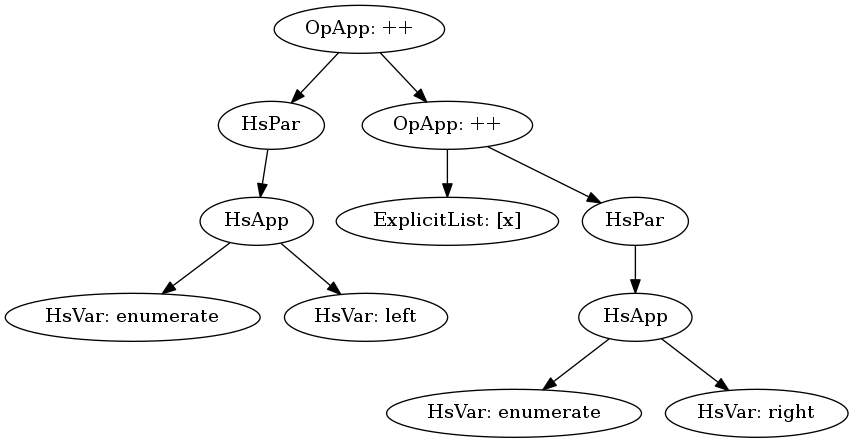
\includegraphics[scale=.5]{graphVis/Chapter3/enumerate.png}
	\end{center}
	\caption{A simplified syntax tree of \texttt{enumerate}'s second case.}
	\label{enumAST}
\end{figure}

The refactoring begins the traversal at the top of the syntax tree with the goal of modifying the entire tree to have a result type of \texttt{DList a}. The root node of the tree is the operator application of the left-hand append operation. This append's result type is the type that determines the whole tree's result type. The standard append operation is paired with the difference list \texttt{DL.append} operation. The refactoring checks to ensure that the difference list append has the correct result type and, because it does, makes the replacement.\footnote{The refactoring will automatically make \texttt{DL.append} infix by surrounding the call with backtick characters since this replacement is modifying an operator application.} After replacing \texttt{++} with \texttt{DL.append}, the result type is correct but the function will no longer type check because \texttt{++} and \texttt{DL.append}'s arguments are not the same types. 

The refactoring then must recurse down both the left and right subtrees to change their types from \texttt{[a]} (the type of \texttt{(++)}'s arguments) to \texttt{DList a} (the type \texttt{append}'s arguments). 

\begin{figure}[h]
	\begin{center}
		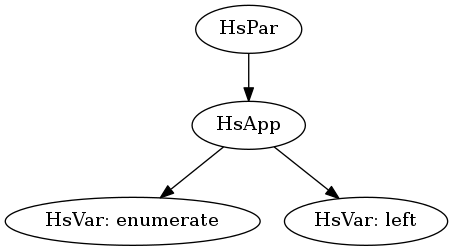
\includegraphics[scale=.5]{graphVis/Chapter3/enumLeft.png}
	\end{center}
	\caption{The left subtree of \texttt{enumerate}'s second case.}
	\label{enumLeft}
\end{figure}

The left subtree of the root node is shown in Figure~\ref{enumLeft}. The refactoring can descend through the parentheses (represented by the \texttt{HsPar} constructor); the refactoring continues down the left side of the function application (\texttt{HsApp}). When the refactoring encounters the call to \texttt{enumerate} it recognises that this is the recursive call and even though the type of \texttt{enumerate} stored in the syntax tree is \texttt{Tree a -> [a]} after the refactoring its type will be \texttt{Tree a -> DList a} which is the correct result type  for this subtree. The refactoring can now confirm that the left subtree is of type \texttt{DList a} without checking the right side of the application because the refactoring didn't change the type of \texttt{enumerate}'s arguments.

\begin{figure}[h]
	\begin{center}
		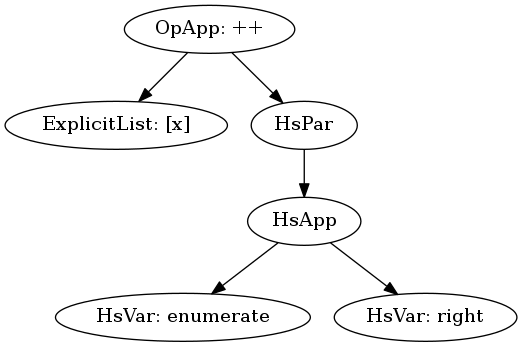
\includegraphics[scale=.5]{graphVis/Chapter3/enumRight.png}
	\end{center}
	\caption{The right subtree of \texttt{enumerate}'s second case.}
	\label{enumRight}
\end{figure}

After refactoring the left subtree, the right subtree needs to be modified to be of type \texttt{DList a} as well. Shown in Figure~\ref{enumRight}, the right subtree's root is the second call to \texttt{(++)}. Once again the refactoring replaces \texttt{++} with \texttt{DL.append} because \texttt{append}'s result type is also \texttt{DList a}. Doing this replacement sets off additional traversals that need to ensure that the two arguments to the root node become typed \texttt{DList a} as well. The right argument to the root of this subtree is the \texttt{(enumerate right)} expression which is handled in the same way the \texttt{(enumerate left)} call was handled. The left subtree of Figure~\ref{enumRight}  is the list literal \texttt{[x]}. This can be replaced with a call to \texttt{(DL.singleton :: a -> DList a)} the equivalent difference list function. At this point the refactoring is finished modifying \texttt{enumerate} and the result can be seen in listing~\ref{enumRef}.

\begin{figure}[t]
\begin{lstlisting}
enumerate :: Tree a -> DList a
enumerate Leaf = empty
enumerate (Node left x right) = (enumerate left) `append` (singleton x) `append` (enumerate right)
\end{lstlisting}
\caption{The refactored definition of \texttt{enumerate}}
\label{enumRef}
\end{figure}

The refactoring is not finished yet, however. The original definition contained in Figure~\ref{enumBefore} had another function \texttt{printEnumTree} that depended on \texttt{enumerate}. The final modification that needs to happen to this example is to wrap all calls to \texttt{enumerate} in \textit{non-refactored} definitions with the abstraction function to convert the result back to a list. The final product of the refactoring can be seen in Figure~\ref{enumFinal}.

\begin{figure}[t]
\begin{lstlisting}
data Tree a = Leaf
            | Node (Tree a) a (Tree a)

enumerate :: Tree a -> DList a
enumerate Leaf = empty
enumerate (Node left x right) = (enumerate left) `append` (singleton x) `append` (enumerate right)

printEnumTree :: (Show a) => Tree a -> IO ()
printEnumTree tree = let lst = toList (enumerate tree) in
  print lst
\end{lstlisting}
\caption{The final product of the refactoring}
\label{enumFinal}
\end{figure}

\subsection{Modifying Parameter and Result Types}

The final case of this refactoring involves modifying both the result type and one (or more) of the parameters of the target function. This example will use the \texttt{explode} function from Figure~\ref{explode} to refactor both its argument and result type to become \texttt{DList a}. \texttt{explode} is a silly function that replicates each of its elements the number of the length of the list, for example, \texttt{explode [1,2,3]} returns \texttt{[1,1,1,2,2,2,3,3,3}. This is an odd function but is has two characteristics we are interested in both its parameter and result type are of type list and it uses the \texttt{map} higher ordered function which is an interesting case for this refactoring. The abstract syntax tree of \texttt{explode} is in Figure~\ref{explode}.

\begin{figure}[t]
\begin{lstlisting}
explode :: [a] -> [a]
explode lst = concat (map (\x -> replicate (length lst) x) lst)
\end{lstlisting}
\caption{The initial definition of \texttt{explode}}
\label{explode}
\end{figure}


\begin{figure}[h!]
	\begin{center}
		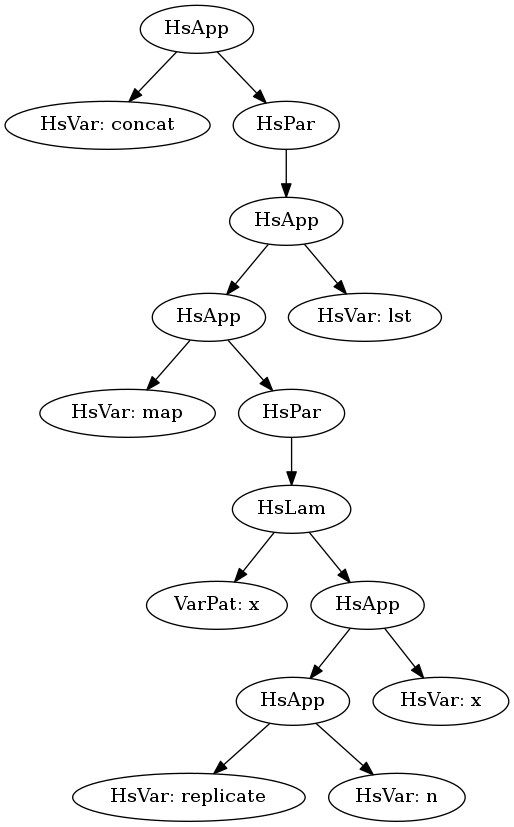
\includegraphics[scale=.5]{graphVis/Chapter3/explode.png}
	\end{center}
	\caption{A simplified representation of \texttt{explodes}'s syntax tree}
	\label{explode}
\end{figure}

Much like the previous case where just the result type was modified, the refactoring will start working on the syntax tree in a top-down manner modifying the function definition to have the correct result type. This case could also be implemented in a bottom-up manner but the top-down method allows for more code reuse from the implementation of the case when the result type is modified.

The refactoring starts on the left subtree with the call to \texttt{concat :: Foldable t => t [a] -> [a]}. The equivalent difference list function is \texttt{DL.concat :: Foldable t => t (DList a) -> DList a} since the result type of this version of \texttt{DL.concat} is \texttt{DList a} the refactoring performs the switch between which function to use. 

After the change on the left subtree, the refactoring needs to modify the right subtree so that it is of type \texttt{Foldable t => t (DList a)} rather than its current type of \texttt{Foldable t => t [a]}. The leftmost child of the right subtree is the call to \texttt{map :: (a -> b) -> [a] -> [b]}. The difference list equivalent map is appropriately typed \texttt{DL.map :: (a -> b) -> DList a -> DList b}. Should the refactoring change this node to the difference list version? And if so what changes will be need to made to other subtrees?

The refactoring will swap this node out if \texttt{Foldable t => t (DList a)} (the type of \texttt{DL.concat}'s parameter) can be the same type as \texttt{DList b}~(\texttt{DL.map}'s result type); since \texttt{DList} is a member of the \texttt{Foldable} type class, the swap can happen as long as the \texttt{b} type variable in \texttt{map}'s type is equal to \texttt{DList a}. This node's type after the swap and filling in the known type variables is: \texttt{DL.map :: (a -> DList b) -> DList a -> DList (DList b)}. This new type's arguments' types are both different from the original types so the refactoring will need to check both of these subtrees as well. 

\begin{figure}[h]
	\begin{center}
		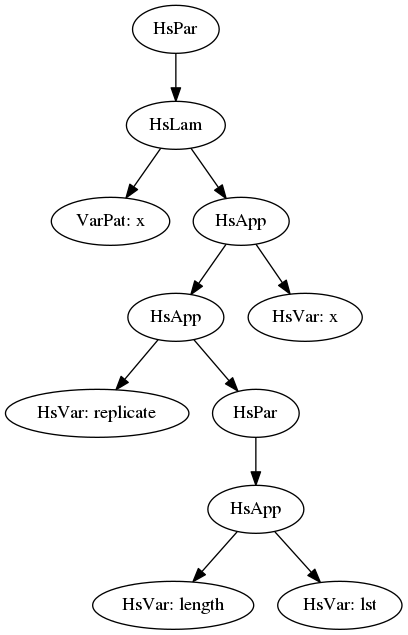
\includegraphics[scale=.5]{graphVis/Chapter3/explodeLam.png}
	\end{center}
	\caption{The syntax tree of the lambda expression in \texttt{explode}.}\label{explodeLam}
\end{figure}

Starting with the lambda expression (the syntax tree in Figure~\ref{explodeLam}) the refactoring needs to modify its type to become \texttt{a -> DList b}\footnote{\texttt{a} and \texttt{b} could be the same type.}. The current type of the lambda expression is \texttt{a -> [a]} so the refactoring only needs to modify its result type. The refactoring can then proceed to the left-most child of this expression, the call to \texttt{replicate :: Int -> a -> [a]}. The refactoring swaps this call for the difference list version of \texttt{DL.replicate :: Int -> a -> DList a}. 

If this refactoring were only modifying the result type of \texttt{explode}, the refactoring would be done modifying the lambda expression because the type change affects the syntax tree in a top down manner. In this case, however, because  the type of \texttt{explode}'s argument was also changed so leaves of the syntax tree can also have changed type. This means that every subtree needs to be checked to ensure that it still type checks.

The untouched sections of this expression's syntax tree are \texttt{replicate}'s arguments. The second argument is just the variable \texttt{x} which hasn't changed type. The first argument on the other hand is the expression \texttt{(length lst)} and \texttt{lst} is the argument of \texttt{explode} that is now a difference list rather than a normal list. Ideally the refactoring would rewrite this expression by replacing the normal list functions (\texttt{length} in this case) with difference list equivalents. Unfortunately there is no difference list version of \texttt{length} so the refactoring will have to introduce the abstraction function to convert back to a normal list to calculate its length. 

The lambda expression has now been successfully refactored. The rewritten lambda expression is in Figure~\ref{lamRef}.\footnote{To help clarify which functions are for lists and which are the difference list versions, all difference list functions have been qualified with the \texttt{DL} identifier.}

\begin{figure}[t]
\begin{lstlisting}
(\x -> DL.replicate (length (DL.toList lst)) x)
\end{lstlisting}
\caption{The refactored lambda expression.}
\label{lamRef}
\end{figure}


Once refactoring the lambda expression is finished there is only a single node of \texttt{explode} that the refactoring hasn't touched yet, the use of \texttt{lst} as the second argument of \texttt{map}. When the refactoring swapped \texttt{map} for its difference list version it was able to determine the new type of both its arguments, \texttt{(a -> DList b)} for the first argument (the lambda expression) and \texttt{DList a} (\texttt{lst}). Fortunately because \texttt{lst} is a target of the refactoring, its new type is \texttt{DList a} so this node can remain unchanged.

\begin{figure}[t]
\begin{lstlisting}
import qualified Data.DList as DL
import Data.DList (DList)

explode :: DList a -> DList a
explode lst = DL.concat 
	(DL.map 
		(\x -> DL.replicate (length (DL.toList lst)) x) 
		lst)
\end{lstlisting} 
\caption{The final refactored result of \texttt{explode}.}
\label{explodeFinal}
\end{figure}

The final result of this case of the Hughes list refactoring is in listing~\ref{explodeFinal}.

\section{Summary}

This chapter has introduced the concept of data-driven refactorings for the object-oriented programming paradigm and described three of the data-driven refactorings developed for this thesis. The first, ``introducing a type signature'', creates an additional abstraction to better describe what types are representing. ``Generalising Maybe'' takes code written for a specific type and generalises it so that it is applicable to more types. Finally the ``list to Hughes list'' refactoring replaces one type with another equivalent type. This refactoring allows a project to be retyped mid-development because it's not always clear from the beginning of a project what the correct data representation should be.

The following chapters will expand on some of these ideas. The next chapter will describe another form of generalisation that rewrites monadic code into its equivalent applicative functor code. The applicative code can be much cleaner and descriptive in certain cases. It can also allow programmers to take advantage of a different way of executing their programs. Chapter~\ref{chp:monadification} discusses introducing effectful abstractions into pure code. This process helps a code base add additional features, such as shared state, mid-development.

\chapter{Implementing Data-Driven Refactorings in HaRe}
\label{chp:generalImp}

\renewcommand{\topfraction}{1}
\renewcommand{\floatpagefraction}{1}

The previous chapter described three refactorings, ``introducing a type synonym,'' ``generalising \texttt{Maybe},'' and the ``list to Hughes list refactorings''. This chapter will describe how refactorings are implemented in HaRe. Section~\ref{sec:genMaybeImp} describes the implementation of the generalising \texttt{Maybe} refactoring which was first covered in Section~\ref{genMaybe}. Section~\ref{sec:hughesListImp} covers the implementation of the ``list to Hughes list'' refactoring (see Section~\ref{listToDlist}) and the embeddable type refactoring system that it is made with. The chapter also covers the enhancements that HaRe's API has undergone while developing the refactorings discussed in this thesis. Section~\ref{hareAPI} discusses the enhancements I made to HaRe's API.

\section{Implementation of the ``Generalising Maybe" refactoring}
\label{sec:genMaybeImp}

The design of the generalising \texttt{Maybe} refactoring was discussed in the previous chapter (see Section~\ref{genMaybe}). This section will describe its implementation in the HaRe refactoring tool. 

This refactoring tries to generalise something of type \texttt{Maybe} to become either of type \texttt{Monad} or \texttt{MonadPlus}. The implementation of this refactoring attempts to produce the ``most general" version of the source program. This means that when possible the refactoring will replace the targetted \texttt{Maybe} type with a value of type \texttt{Monad}; if this is not possible the value will be of type \texttt{MonadPlus}, and finally if that also is not possible the refactoring cannot continue and the source and target programs of the refactoring are identical.

\begin{figure}[t]
\begin{lstlisting}
doMaybeToPlus :: FilePath -> SimpPos -> String -> Int -> RefactGhc ()  
doMaybeToPlus fileName pos@(row,col) funNm argNum = do
  parsed <- getRefactParsed
  let mBind = getHsBind pos parsed
  case mBind of
   Nothing -> error "Function bind not found"
   Just funBind -> do
       hasNtoN <- containsNothingToNothing funNm argNum pos funBind
       case hasNtoN of
         True -> do
           doRewriteAsBind fileName pos funNm
         False -> do 
           canReplaceConstructors <- isOutputType funNm argNum pos funBind
           case canReplaceConstructors of
             True -> do
               logm $ "Can replace constructors"
               replaceConstructors pos funNm argNum
             False -> return ()
       return ()
\end{lstlisting} 
\caption{The top level function of the generalising \texttt{Maybe} refactoring.}
\label{genMaybeTopLevel}
\end{figure}

This refactoring, at the top level (defined in figure~\ref{genMaybeTopLevel}), determines which type the target program can be generalised to. This is determined by whether the target function contains a ``\texttt{Nothing} to \texttt{Nothing}" case. When this is true then the function can be rewritten with the \texttt{Monad} interface. This check is defined in the \texttt{containsNothingToNothing} function, which traverses the AST of the target function searching for a case where the \texttt{Pat} on the left hand side pattern is only \texttt{Nothing} and the \texttt{HsExpr} on the right hand side of the match is only \texttt{Nothing}. If this is true for the target function then \texttt{doRewriteAsBind} modifies the other case(s) of the function.

The other case has the refactoring checking if its possible to replace all of \texttt{Maybe}'s constructors with the equivalent \texttt{MonadPlus} values. This is checked in \texttt{isOutputType} which checks whether the target type of the refactoring is also the result type of the function. When this is the case \texttt{MonadPlus}' constructors can be substituted for \texttt{Maybe}'s \texttt{Nothing} and \texttt{Just}. This is done by the \texttt{replaceConstructors} function.

The rest of this section will discuss the two functions that modify the source function, \texttt{doRewriteAsBind} and \texttt{replaceConstructors}. There will also be a brief section on enhancements that can be made to this implementation of the generalise \texttt{Maybe} refactoring to make it more robust.

\subsection{Generalising to \texttt{Monad}}

\begin{figure}[t]
\begin{lstlisting}
doRewriteAsBind :: FilePath -> SimpPos -> String -> RefactGhc ()
doRewriteAsBind fileName pos funNm = do
  parsed <- getRefactParsed
  let bind = gfromJust "doRewriteAsBind" $ getHsBind pos parsed
      matches = GHC.mg_alts . GHC.fun_matches $ bind
  if (length matches) > 1
    then error "Multiple matches not supported"
    else do
    let (GHC.L _ match) = head matches
    (varPat, rhs) <- getPatAndRHS match
    (newPat, _) <- liftT $ cloneT varPat
    (newRhs, _) <- liftT $ cloneT rhs
    let rhs = justToReturn newRhs
    lam <- wrapInLambda newPat rhs
    let newNm = case newPat of
                     (GHC.L _ (GHC.VarPat nm)) -> mkNewNm nm
                     _ -> mkRdrName $ "m_value_" ++ funNm
    new_rhs <- createBindGRHS newNm lam
    replaceGRHS funNm new_rhs newNm
    fixType funNm
      where mkNewNm rdr = let str = GHC.occNameString $ GHC.rdrNameOcc rdr in
              GHC.Unqual $ GHC.mkVarOcc ("m_" ++ str)
\end{lstlisting}
\caption{The implementation of \texttt{doRewriteAsBind}. The function that generalises \texttt{Maybe} to \texttt{Monad}}
\label{doRewriteAsBind}
\end{figure}

Figure~\ref{doRewriteAsBind} shows the implementation of \texttt{doRewriteAsBind} the function that rewrites a function of type \texttt{Maybe} to use the monadic bind interface instead. The first three lines of \texttt{doRewriteAsBind} (lines 3-6 in figure~\ref{doRewriteAsBind}) extract the list of matches that make up every Haskell function. A match consists of the left hand side pattern binding and the right hand side expression. For example, in figure~\ref{matchExample}, the \texttt{last} function's AST representation consists of three matches, one for each function body, whereas the AST of \texttt{doRewriteAsBind} only has one match because its definition contains only a single body.

Once the target function's list of matches is retrieved \texttt{doRewriteAsBind} can then perform the appropriate refactoring for a target function with a single match or multiple matches\footnote{It's important to note that \texttt{containsNothingToNothing}, the function that checks if the target function has a \texttt{Nothing} to \texttt{Nothing} case, also removes this case from the AST. This means that the \texttt{matches} list excludes this case.}. Currently this implementation does not support multiple matches but the refactoring could be expanded to automatially wrap the target function's pattern matches in a \texttt{case} statement. Another way to allow HaRe to support this case is to create a separate refactoring that rewrites functions with multiple bindings to use a \texttt{case} statement instead, which would allow the refactoring to proceed.

\begin{figure}[t]
\begin{lstlisting}
last :: [a] -> Maybe a
last [] = Nothing
last [x] = Just x
last (x:xs) = last xs
\end{lstlisting}
\caption{The AST of the \texttt{last} function contains three matches.}
\label{matchExample}
\end{figure}

After checking that there is only a single match in the AST of the target function, \texttt{doRewriteAsBind} can start modifying that function. The rest of \texttt{doRewriteAsBind} (from line 10 in figure~\ref{doRewriteAsBind}) constructs a lambda expression and variable to make up the new right hand side of the target function. 

This is done by taking the right hand side expression from the target function's match and replacing any calls to \texttt{Just} with \texttt{return}. This generalised version of the right hand side expression can then be wrapped in a lamdba expression with the original pattern being the binding for this expression (line 14's call to \texttt{wrapInLambda}). This new lambda expression can be bound to the newly created variable \texttt{newNm}. This new variable keeps the name given to the original pattern if it was just a simple name (e.g. ``\texttt{x}'') and appends ``\texttt{m\char`_}'' to this name to prevent a naming conflict with the variable inside of the lambda expression. In the case that the pattern was more complex, like when matching a data type constructor (e.g. \texttt{Just x}) or a list \texttt{(x:xs)}, then a generic variable name is created using the target function's name.\footnote{The user of the refactoring will most likely want to apply the renaming refactoring to this variable to give it a more appropriate name.}

The new name is then bound to the lambda expression (line 18) and the target function's body is replaced with this bind expression. The step of the rewriting generalises the type signature to be use the \texttt{Monad} type class in the place of \texttt{Maybe}.

\subsection{Generalising to \texttt{MonadPlus}}

When the target function cannot be generalised to \texttt{Monad} because it does not contain the \texttt{Nothing} to \texttt{Nothing} case, it may be possible to generalise it to use the \texttt{MonadPlus} typeclass instead. This section will cover how this case of the refactoring is implemented in HaRe.

An instance of \texttt{MonadPlus} is a \texttt{Monad} with a monoidal structure.
This structure is defined by an associative operator \texttt{mplus} and its identity value \texttt{mzero}~\citep{typeclassopedia}. 
In \texttt{Maybe}'s case \texttt{mzero} is defined as \texttt{Nothing} and \texttt{Maybe}'s other constructor, \texttt{Just}, is the value of \texttt{Maybe}'s definition \texttt{return}.
This case of the refactoring just replaces instances of \texttt{Just} with \texttt{return} and \texttt{Nothing} with \texttt{mzero}. 

\begin{figure}[t]
\begin{lstlisting}
replaceConstructors :: SimpPos -> String -> Int -> RefactGhc ()
replaceConstructors pos funNm argNum = do
  parsed <- getRefactParsed
  let (Just bind) = getHsBind pos parsed
  newBind <- applyInGRHSs bind replaceNothingAndJust
  replaceBind pos newBind
  fixType' funNm argNum
    where applyInGRHSs :: (Data a) => UnlocParsedHsBind -> (a -> RefactGhc a) -> RefactGhc UnlocParsedHsBind
          applyInGRHSs parsed fun = applyTP (stop_tdTP (failTP `adhocTP` (runGRHSFun fun))) parsed
          runGRHSFun :: (Data a) => (a -> RefactGhc a) -> ParsedGRHSs -> RefactGhc ParsedGRHSs
          runGRHSFun fun grhss@(GHC.GRHSs _ _) = SYB.everywhereM (SYB.mkM fun) grhss
          mzeroOcc = GHC.mkVarOcc "mzero"
          nothingOcc = GHC.mkVarOcc "Nothing"
          returnOcc = GHC.mkVarOcc "return"
          justOcc = GHC.mkVarOcc "Just"
          replaceNothingAndJust :: GHC.OccName -> RefactGhc GHC.OccName
          replaceNothingAndJust nm
            | (GHC.occNameString nm) == "Nothing" = do
                logm "Replacing nothing"
                return mzeroOcc
            | (GHC.occNameString nm) == "Just" = do
                logm "Replace just"
                return returnOcc            
            | otherwise = return nm
\end{lstlisting}
\caption{The \texttt{replaceConstructors} function replaces \texttt{Maybe}'s constructors with more general values.}
\label{replaceConstructors}
\end{figure}

Figure~\ref{replaceConstructors} shows the top level function \texttt{replaceConstructors} that modifies a target function to replace the \texttt{Maybe} specific values with \texttt{mzero} and \texttt{return}. This function primarily consists of two traversal patterns, the ``stop top down traversal'' (\texttt{stop\_tdTP}) in \texttt{applyInGRHSs} and the \texttt{everywhereM} in \texttt{runGRHSFun}. The only parts of the function that need to be changed are in the right hand side of the target function; the first traversal (from \texttt{applyInGRHSs}) descends to this level and then stops when the guarded right hand side type is found. From there the other traversal continues down the tree replacing the instances \texttt{Just} and \texttt{Nothing}.

After the right hand side binding has been rewritten, the target function's original binding is replaced with the new binding in the call to \texttt{replaceBind} on line six of figure~\ref{replaceConstructors}. Replacing the original binding of a function with a refactoring one is a common operation that many refactorings need to perform. Due to its re-usability \texttt{replaceBind} is a function from HaRe's API and will be discussed in section~\ref{hareAPI}. 

The final step of this refactoring changes the type signature of the target function. The instances of \texttt{Maybe} in the type signature need to be replaced with a type variable that is bound to the \texttt{MonadPlus} typeclass. The \texttt{fixType'} function performs this rewriting. The definition of \texttt{fixType'} is shown in figure~\ref{fixTypePrime}.

\begin{figure}[t]
\begin{lstlisting}
fixType' :: String -> Int -> RefactGhc ()
fixType' funNm argPos = do
  logm "Fixing type"
  parsed <- getRefactParsed
  let m_sig = getSigD funNm parsed
      (GHC.L sigL (GHC.SigD sig)) = gfromJust "fixType'" m_sig
  fixedClass <- fixTypeClass sig
  replacedMaybe <- replaceMaybeWithVariable fixedClass
  newSig <- locate (GHC.SigD replacedMaybe)
  addNewKeyword ((G GHC.AnnDcolon), DP (0,1)) newSig
  synthesizeAnns newSig
  addNewLines 2 newSig
  newParsed <- replaceAtLocation sigL newSig
  anns <- liftT getAnnsT
  putRefactParsed newParsed anns         
\end{lstlisting}
\caption{\texttt{fixType'} is a function that fixes the type signature of a function that is being generalised from \texttt{Maybe} to \texttt{MonadPlus}.}
\label{fixTypePrime}
\end{figure}

The definition of \texttt{fixType'} is shown in figure~\ref{fixTypePrime}, this functions follows the following steps:

\begin{itemize}
\item \textit{Line 5:} Retrieve the signature from the parsed abstract syntax
\item \textit{Line 7:} Insert the binding of the variable ``\texttt{m}'' to the \texttt{MonadPlus} typeclass
\item \textit{Line 8:} Replace the instances of \texttt{Maybe} with the ``\texttt{m}'' type variable
\item \textit{Lines 9 - 12:} Create the appropriate annotations for the new syntax elements
\item \textit{Line 13:} Replaces the old type signature in the parsed source
\item \textit{Line 15:} Updates the refactoring state with the modified parsed source
\end{itemize}

The \texttt{fixTypeClass} and \texttt{replaceMaybeWithVariable} functions transform the abstract syntax of the type signature, and the rest of \texttt{fixType'} creates and modifies the associated annotations so that all of its elements appear in the target program and are well formatted. For example, the call to \texttt{addNewKeyword} on line 10 of figure~\ref{fixTypePrime} associates the \texttt{AnnDcolon} annotation with the new type signature. This annotation represents the ``\texttt{::}'' operator that is otherwise not represented explicitly in the abstract syntax tree. These annotations are what is used by ghc-exactprint to determine where syntax elements that are not located by the abstract syntax are and how the target module should be formatted. This was discussed in more detail in section~\ref{ghcExactprint}.

This section has covered the implementation of the generalising \texttt{Maybe} refactoring. This is a fairly straightforward refactoring implementation, the preconditions are checked up front and depending on the structure of the target function the correct transformation is chosen. The next section will describe the implementation of the ``list to Hughes list'' refactoring. This refactoring must descend the entire syntax tree of each target function and transformations may occur based on the type of the AST's subtrees.  

\section{Implementation of the ``List to Hughes List" refactoring}
\label{sec:hughesListImp}

The ``list to Hughes list'' refactoring was first described in section~\ref{listToDlist}. This section will describe the implementation of that refactoring in HaRe. Section~\ref{listToDlist} also introduced the concept of a type that can be ``embedded'' into another. This means that the source type, which in this particular case is \texttt{[a]}, can be transformed into the target type (\texttt{DList a}) and the original value of the object can be retrieved from the target type.

Though ``list to Hughes list'' is the specific refactoring outlined in this thesis and implemented in HaRe, this sort of refactoring can be applied to any pair of types that hold the properties described in section~\ref{listToDlist}. HaRe's implementation of the ``list to Hughes list'' refactoring keeps this in mind and efforts were made to build reusable components so that similar refactorings can be easily implemented for different types.

The \texttt{doHughesList} function shown in figure~\ref{doHughesList} is main function that performs the ``list to Hughes list'' refactoring. This function performs four primary tasks, adding the import declaration for the difference list library, transforming the function definition, replacing the existing function definition, and wrapping the call points of the target function with the abstraction function.

\begin{figure}[t]
\begin{lstlisting}
doHughesList :: FilePath -> String -> SimpPos -> Int -> EmbFuncStrings -> RefactGhc ()
doHughesList fileName funNm pos argNum fStrs = do
  let mqual = Just "DList"
  addSimpleImportDecl "Data.DList" mqual
  ty <- getDListTy mqual
  parsed <- getRefactParsed
  let
    (Just lrdr) = locToRdrName pos parsed
    rdr = GHC.unLoc lrdr
    dlistCon = getTyCon ty
    newFType = resultTypeToDList dlistCon 
    (Just funBind) = getHsBind rdr parsed
    (Just tySig) = getTypeSig pos funNm parsed
    newResTy = getResultType ty
  iDecl <- dlistImportDecl mqual
  iSt <- getInitState iDecl fStrs "toList" "fromList" mqual newResTy
  bind' <- embRefact argNum mqual rdr ty iSt funBind
  replaceFunBind pos bind'
  newTySig <- fixTypeSig argNum tySig
  replaceTypeSig pos newTySig
  let modQual = case mqual of
                  (Just s) -> s ++ "."
                  Nothing -> ""
  fixClientFunctions modQual (numTypesOfBind funBind) argNum rdr
  addConstructorImport
\end{lstlisting}
\caption{\texttt{doHughesList} is the top level function of the Hughes list refactoring.}
\label{doHughesList}
\end{figure}

The most interesting part of this refactoring is the transformation of the function definition. The other steps are handled by HaRe's API which is discussed in section~\ref{hareAPI}. The transformation occurs on lines 16 and 17 of figure~\ref{doHughesList}. The transformation runs within its own state and line 16 creates the initial value of this state while line 17 actually runs the stateful computation. The state's type is shown in figure~\ref{embState}.

\begin{figure}[t]
\begin{lstlisting}
data EmbRefactState = EmbState {
  funcs :: EmbeddableFuncs,
  typeStack :: [Maybe GHC.Type],
  insertAbs :: Bool
                               }
                               
data EmbeddableFuncs = IF {
  projFun :: GHC.RdrName,
  absFun :: GHC.RdrName,
  eqFuns :: M.Map String (GHC.RdrName, GHC.Type)
  }
\end{lstlisting}
\caption{The type of the state that the refactoring runs in.}
\label{embState}.
\end{figure}

The state consists of three fields, \texttt{funcs} keeps track of the functions that operate over the source type and their equivalent functions that operate on the target type, and the names of the projection and abstraction functions. The \texttt{typeStack} field is a stack that keeps track of what changes need to be made further down the abstract syntax tree. The type stack is described in more detail in section~\ref{typeStack} below. Finally, the \texttt{insertAbs} field keeps track of when the abstraction function needs to be applied to certain values.

The call to \texttt{getInitState} on line 16 of figure~\ref{doHughesList} takes in the import declaration of the target type, a list of pairs of strings that represent the equivalent functions over the source and target types, the names of the projection and abstraction functions, the target type's import qualifier if it exists, and the final result type of the target function. In the ``list to Hughes list'' case the import declaration is ``\texttt{import Data.DList qualified as DList}.'' Because many of the Hughes list functions have the same names as their normal list counterparts a qualifier is required so \texttt{DList} is chosen. 

The list of pairs associates the normal list functions with the appropriate Hughes list functions. A single pair in this list contains, first, the normal list function name followed by the Hughes list function that performs the same operation. For example, ``\texttt{(:)}'' is paired with its Hughes list equivalent ``\texttt{cons}'' because both functions add a single element to the beginning of a list. The full list of pairs for the ``list to Hughes list'' refactoring is shown in figure~\ref{assocFuns}.

\begin{figure}[t]
\begin{lstlisting}
[("[]","empty"),(":","cons"),("++","append"),("concat", "concat"),("replicate","replicate"), ("head","head"),("tail","tail"),("foldr","foldr"),("map","map"), ("unfoldr", "unfoldr")]
\end{lstlisting}
\caption{The list of associated function pairs for the ``list to Hughes list'' refactoring}
\label{assocFuns}
\end{figure} 

The projection and abstraction functions are ``\texttt{toList}'' and ``\texttt{fromList}'' respectively in the ``list to Hughes list'' case. The final result type of the target function depends on the result type of the source function. If the result type of the source function is \texttt{[Int]} then the result type of the target function will be \texttt{DList Int}, if the source function's result type is \texttt{[a]} then the target function's result type will be \texttt{DList a}.

Once the initial state has been created the transformation is performed in a top down, left to right manner with the call to \texttt{embRefact} on line 17 of figure~\ref{doHughesList}. As seen in figure~\ref{embRefact} the definition of \texttt{embRefact} simply calls the API function \texttt{modMGAltsRHS} which applies a function that modifies an expression to each of the right hand side values of the given function binding. The ``real'' work of the transformation occurs in \texttt{doEmbRefact} which is defined in figure~\ref{doEmbRefact}.

\begin{figure}[t]
\begin{lstlisting}
embRefact :: Int -> Maybe String -> GHC.RdrName -> GHC.Type -> EmbRefactState -> ParsedBind -> RefactGhc ParsedBind
embRefact _ mqual funNm newFTy iST bnd = modMGAltsRHS (\e -> runEmbRefact (doEmbRefact e) iST) bnd
\end{lstlisting}
\caption{The definition of \texttt{embRefact}}
\label{embRefact}
\end{figure}

\begin{figure}[t]
\begin{lstlisting}
doEmbRefact :: ParsedLExpr -> EmbRefact ParsedLExpr
doEmbRefact expr = do
  b1 <- embDone
  b2 <- skipCurrent
  if b1 || b2
    then do
    lift $ logm "Skipping this expr: "
    lift $ logm (SYB.showData SYB.Parser 3 expr)
    return expr
    else doEmbRefact' expr
  where doEmbRefact' :: ParsedLExpr -> EmbRefact ParsedLExpr
  		doEmbRefact' = ...
\end{lstlisting}
\caption{\texttt{doEmbRefact} is the function that transforms a given expression to use the target type.}
\label{doEmbRefact}
\end{figure}

The top level, \texttt{doEmbRefact}, function controls when the traversal stops, the helper function \texttt{doEmbRefact'} is what actually transforms the given expression based on its constructor. The two stop conditions, \texttt{b1} and \texttt{b2} from figure~\ref{doEmbRefact} lines three and four, are determined by the state of the ``type stack''.

\subsection{The goal type stack}
\label{typeStack}

The type stack is part of the refactoring's state and is of type \texttt{[Maybe GHC.Type]} each member of the stack represents the type that a sub tree must be changed to. The stack will be initialised with a single value ``\texttt{Just (DList a)}'' where \texttt{a} is the type of list from the source function this is because the result type of the entire syntax tree needs to be changed to \texttt{Just (DList a)}. The stack keeps track the ``goal types'' of each sub-tree. 

Consider the \texttt{enumerate} example from section~\ref{hugesListResTy}, which is shown here again in figure~\ref{enumerate2}.

\begin{figure}[t]
\begin{lstlisting}
data Tree a = Leaf
            | Node (Tree a) a (Tree a)

enumerate :: Tree a -> [a]
enumerate Leaf = []
enumerate (Node left x right) = (enumerate left) ++ [x] ++ (enumerate right)

\end{lstlisting}
\caption{Definition of enumerate}
\label{enumerate2}
\end{figure}

When refactoring the result type of \texttt{enumerate} to become \texttt{DList a} the refactoring begins at the root of \texttt{enumerate}'s abstract syntax tree and the goal type stack is initialised as \texttt{[Just (DList a)]}. At the start of this refactoring the goal type stack holds the single type that the root node needs to become. The initial state of the stack and the abstract syntax tree is shown in figure~\ref{initASTStack}.

\begin{figure}[t]
	\begin{subfigure}{\linewidth}
		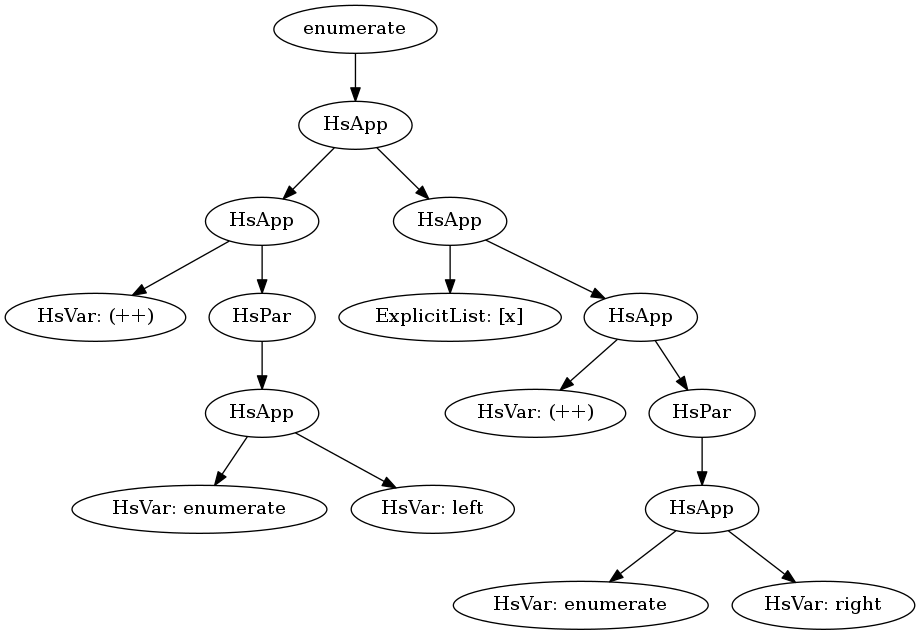
\includegraphics[scale=.5]{graphVis/Chapter4/enumerate.png}
	\end{subfigure}\par\medskip

	\begin{subfigure}{\linewidth}
		\begin{lstlisting}[mathescape]
			typeStack = [Just (DList a)$^1$]
		\end{lstlisting}
	\end{subfigure}\par\medskip
\caption{The initial state of the AST and goal type stack}
\label{initASTStack}
\end{figure} 

In this case the root node of the AST can be replaced with a call to \texttt{DList.append} because this functions result type matches the goal type for the node and \texttt{DList.append} is paired with \texttt{++} the current value of the node. Once the root node is replaced with the call to \texttt{DList.append} the current value of the stack is popped off and \texttt{Just (DList a)} is pushed onto the stack twice. This is because \texttt{(++)} takes in two arguments both of type \texttt{[a]} whereas \texttt{DList.append}'s two arguments need to be of type \texttt{DList a}. The refactoring continues by changing the root node's left child first. The goal type of this subtree is \texttt{DList a} and so the refactoring traverses down to the leftmost child of this subtree. The state of the refactoring at this point in shown in figure~\ref{enumStateL1}.

\begin{figure}[t]
	\begin{subfigure}{\linewidth}
		\includegraphics[scale=.5]{graphVis/Chapter4/enumerateL1.png}
	\end{subfigure}\par\medskip

	\begin{subfigure}{\linewidth}
		\begin{lstlisting}[mathescape]
			typeStack = [Just (DList a)$^1$, Just (DList a)$^2$]
		\end{lstlisting}
	\end{subfigure}\par\medskip
\caption{After replacing the root node the refactoring must resolve the types of its subtrees.}
\label{enumStateL1}
\end{figure} 

When the refactoring reaches the call to \texttt{enumerate}, it realises that this is a recursive call so the result type is already \texttt{DList a} so no change needs to be made and the top of the goal type stack can be popped off. Also since \texttt{enumerate}'s argument is not a target of the refactoring, those subtrees will not need to be traversed. This is indicated by pushing \texttt{Nothing} onto the stack (see figure~\ref{enumStateL2}). This means that the entire left child of the root node is correct after the change to the root node and the refactoring can begin working on the right child of the root node.

\begin{figure}[t]
	\begin{subfigure}{\linewidth}
		\includegraphics[scale=.5]{graphVis/Chapter4/enumerateL2.png}
	\end{subfigure}\par\medskip

	\begin{subfigure}{\linewidth}
		\begin{lstlisting}[mathescape]
			typeStack = [Nothing$^1$, Just (DList a)$^2$]
		\end{lstlisting}
	\end{subfigure}\par\medskip
\caption{The \texttt{Nothing} on top of the type stack means that the right hand side of the application of \texttt{enumerate} doesn't need to be checked. The \texttt{Nothing} can be popped off the type stack and the traversal continues upwards.}
\label{enumStateL2}
\end{figure}

The first node that the refactoring encounters when traversing the right child of the root node is another application of \texttt{++}. This is handled in the same that its parent node was, with \texttt{DList.append} replacing \texttt{++} and the new types of its subtrees (\texttt{DList a} in this case) pushed onto the stack. In the same way that the root node was handled, the refactoring begins by traversing the left subtree. The state of the refactoring at this point is shown in figure~\ref{enumStateR1}.

\begin{figure}[t]
	\begin{subfigure}{\linewidth}
		\includegraphics[scale=.5]{graphVis/Chapter4/enumerateR1.png}
	\end{subfigure}\par\medskip

	\begin{subfigure}{\linewidth}
		\begin{lstlisting}[mathescape]
			typeStack = [Just (DList a)$^1$, Just (DList a)$^2$]
		\end{lstlisting}
	\end{subfigure}\par\medskip
\caption{Traversing the left child again to fix the calls to the newly inserted \texttt{DList.append}.}
\label{enumStateR1}
\end{figure}

The node that the refactoring is at is a singleton list expression and according to the goal type stack it must be re-typed to \texttt{DList a}. Fortunately the \texttt{DList} library provides a \texttt{singleton} function that produces a Hughes list of length one from a single parameter. The explicit list can be replaced with a call to \texttt{DList.singleton} and this subtree is now correctly typed and the top of the goal type stack can be popped (see figure ~\ref{enumStateR2}).

\begin{figure}[t]
	\begin{subfigure}{\linewidth}
		\includegraphics[scale=.4]{graphVis/Chapter4/enumerateR2.png}
	\end{subfigure}\par\medskip

	\begin{subfigure}{\linewidth}
		\begin{lstlisting}[mathescape]
			typeStack = [Just (DList a)$^1$]
		\end{lstlisting}
	\end{subfigure}\par\medskip
\caption{The subtree representing the explicit list has been replaced with a call to \texttt{DList.singleton}.}
\label{enumStateR2}
\end{figure}

The only part of the AST that hasn't been refactored is the right most expression ``\texttt{(enumerate right)}''. This expression will be handled in the same way that the first recursive call to \texttt{enumerate} was. The refactoring will descend to the call to \texttt{enumerate}, pop the top of the goal type stack and push \texttt{Nothing} onto the stack because none of the arguments need to change. The refactoring will ascend to the \texttt{HsApp} node and pop off the \texttt{Nothing} value, and therefore not descend to check the subtree constisting only of the \texttt{right} variable. At this point the goal type stack is empty so the refactoring is finished and can return the modified AST.

This section has given a concrete example of how an abstract syntax tree is traversed and how the goal type stack is used. The next section will go through the code that handles each of the different types of expressions.

\subsection{Traversing an expression, the implementation of \texttt{doEmbRefact'}}

Though the top level \texttt{doEmbRefact} function determines if a subtree should be changed at all, \texttt{doEmbRefact'} determines how the transformation traverses the subtree and the changes that occur based on the constructor of the current abstract syntax node. This section discusses each of the cases of \texttt{doEmbRefact'}.

\begin{figure}[t]
\begin{lstlisting}
        doEmbRefact' (GHC.L l (GHC.HsApp le re)) = do
          le' <- doEmbRefact le
          wrapWithProj <- shouldInsertProj       
          re' <- doEmbRefact re
          lift $ logm "POST RHS REFACT IN APP CASE"
          let newApp = (GHC.L l (GHC.HsApp le' re'))
          if wrapWithProj
            then do
            projRdr <- getProjFun
            let var = GHC.HsVar projRdr
            pApp <- lift $ wrapInPars newApp
            lVar <- lift $ locate var
            lift $ addAnnVal lVar
            let fullApp = GHC.HsApp lVar pApp
            lift $ locate fullApp
            else return newApp
\end{lstlisting}
\caption{The case of \texttt{doEmbRefact'} that handles function applications.}
\label{embRefactApp}
\end{figure}

The way that function applications are transformed is shown in figure~\ref{embRefactApp}. The refactoring will transform the left hand side of the application first, then it checks if the entire application needs to be wrapped with a call to the projection function because the leftmost child of the subtree does not have an equivalent function over the target type. After that the right sub tree is refactored and this refactored expression is applied to the refactored left hand expression.

If the projection function needs to be introduced at this layer then another application is wrapped around the already modified syntax tree. Otherwise the application with its modified sub trees can just be returned.

\begin{figure}[t]
\begin{lstlisting}
        doEmbRefact' (GHC.L l (GHC.OpApp le op rn re)) = do
          op' <- doEmbRefact op
          wrapWithProj <- shouldInsertProj
          lift $ addBackquotes op'
          le' <- doEmbRefact le
          re' <- doEmbRefact re
          let newOp = (GHC.L l (GHC.OpApp le' op' rn re'))
          wrapProjIfNeeded wrapWithProj newOp
\end{lstlisting}
\caption{The case of \texttt{doEmbRefact'} that handles operator applications}
\label{embRefactOp}
\end{figure}

The next case, operator application, is handled much like function application is: whether or not the operator can be replaced by a target type equivalent determines if the projection function needs to be added. Otherwise the left- and right-hand expressions can be refactored. 

The new operator may not be allowed in an infix position and in this case backquotes (\texttt{`}) are added, which in Haskell makes a prefix function into an infix version of that function. A good example of this is \texttt{DList.append}. \texttt{DList.append} is paired with \texttt{(++)} which is an operator whereas \texttt{DList.append} is a prefix function, therefore the refactoring of ``\texttt{leftList ++ rightList}'' is ``\texttt{leftListRef `DList.append` rightListRef}'' where \texttt{leftListRef} and \texttt{rightListRef} are the refactored parameters to the append function.

\begin{figure}[!t]
\begin{lstlisting}
        doEmbRefact' var@(GHC.L l (GHC.HsVar rdr)) = do
          st <- get          
          let ts = typeStack st
              fs = funcs st              
          typed <- lift getRefactTyped
          mId <- lift (getIdFromVar var)
          let id = gfromJust ("Tried to get id for: " ++ SYB.showData SYB.Parser 3 rdr) mId
              currTy = GHC.idType id
              keyOcc = GHC.rdrNameOcc rdr
              mVal = (GHC.occNameString keyOcc) `M.lookup` (eqFuns fs)
          case mVal of
            Nothing -> do
              popTS
              dontSearchSubTrees currTy
              lift $ logm "Nothing case of mVal"
              printStack
              insertProjToT
              return var
            (Just (oNm, ty)) -> do
                let changedTypes = typeDifference ty currTy
                    newE = (GHC.L l (GHC.HsVar oNm))
                oldAnns <- lift fetchAnnsFinal
                case M.lookup (mkAnnKey var) oldAnns of
                  Nothing -> lift (mergeRefactAnns $ copyAnn var newE oldAnns)
                  Just v -> do
                    let dp = annEntryDelta v
                    lift $ addAnnValWithDP newE dp
                popTS
                addToTS changedTypes                
                return newE
\end{lstlisting}
\caption{The case of \texttt{doEmbRefact'} that handles variables}
\label{embRefactVar}
\end{figure}

The major changes that the refactoring makes are performed when \texttt{doEmbRefact'} encounters a variable. This logic is shown in figure~\ref{embRefactVar}. The first six lines of this case (lines 2 through 7 in figure~\ref{embRefactVar}) retrieve the type of the current variable from the typed abstract syntax. 

Next (line 10 of figure~\ref{embRefactVar}) the refactoring checks if there is a possible replacement function. If a replacement is not available then the transformation can pop the top element from the stack and any parameters that are applied to this value don't have to be searched. This is done through the call to \texttt{dontSearchSubTrees} which puts \texttt{Nothing} values onto the type stack. For example, if the current variable was ``\texttt{f :: a -> b -> c}'' and there was no possible replacement for \texttt{f}, then \\ \texttt{dontSearchSubTrees} would push two \texttt{Nothing}s onto the type stack so that the subtrees of type \texttt{a} and \texttt{b} aren't modified. Finally in this case the boolean ``\texttt{insertProj}'' in the refactoring state is flipped, which informs the refactoring that higher up the tree the application of this value needs to be wrapped with the projection function. 

When a possible replacement for the current value is found (this case begins on line 19 of figure~\ref{embRefactVar}), the refactoring first calculates which parameters of the new function have different types from the original function which is stored in the \texttt{changedTypes} variable. This variable is a list of \texttt{Maybe GHC.Type}s where the \texttt{Nothing} values mean that the type of that parameter has not changed and ``\texttt{Just \_}'' values indicate the new type that the parameter must become. This list represents each parameter of the variable from left to right order. This list of type changes that need to be handled is pushed onto the type stack in line 29 of figure~\ref{embRefactVar} after the current goal type is popped from the stack. 

The rest of this case constructs the new expression and copies over the annotation from the old piece of abstract syntax so that any formatting associated with the original call is preserved in the new source code. Finally the new expression can be returned.

\begin{figure}[t]
\begin{lstlisting}
        doEmbRefact' eLst@(GHC.L l (GHC.ExplicitList ty mSyn lst)) = do
          if (length lst) == 1
            then do
            st <- get
            let fs = funcs st
                singletonRdr = mkQualifiedRdrName (GHC.mkModuleName "DList") "singleton"
                singletonVar = (GHC.HsVar singletonRdr)
            lVar <- lift $ locate singletonVar
            lift $ addAnnVal lVar
            lift $ zeroDP lVar
            let rhs = head lst
            lift $ setDP (DP (0,1)) rhs
            lApp <- lift $ locate (GHC.HsApp lVar rhs)
            parApp <- lift $ wrapInPars lApp
            return parApp
            else do
            st <- get
            let fs = funcs st
                projRdr = projFun fs
            lVar <- lift $ locate (GHC.HsVar projRdr)
            lApp <- lift $ locate (GHC.HsApp lVar eLst)
            lift $ wrapInPars lApp
            return lApp
\end{lstlisting}
\caption{The case that handles explicit list syntax}
\label{embRefactExpLst}
\end{figure}

One of the goals that influenced the design of this system was to produce a reusable system so that more embeddable type refactorings could easily be created. A tricky situation arises with Haskell's support for explicit list syntax (e.g. ``\texttt{[1,2,3]}''). Because lists are the source type of the ``list to Hughes list'' refactoring, the explicit list syntax may need to be transformed during the refactoring, so this type-specific bit of code remains in the otherwise generic function. Ideally this function could remain completely type agnostic but because the ``list to hughes list'' refactoring works over the list type it needs to descend into this type specific constructor of the abstract syntax tree.

The case that handles explicit lists is shown in figure~\ref{embRefactExpLst} and is simple enough. If the explicit list is just a single element long (e.g. ``\texttt{[3]}'') then that value will be passed to the difference list's \texttt{singleton} function, otherwise the projection function is wrapped around longer lists. 

Finally \texttt{doEmbRefact'} has a simple catch-all case that handles all the other constructors of \texttt{HsExpr}. This case shown in figure~\ref{doEmbCatchAll} uses the \texttt{gmapM} generic combinator to recursively call \texttt{doEmbRefact} on all of the given expression's children. 

\begin{figure}[t]
\begin{lstlisting}
doEmbRefact' ex = gmapM (SYB.mkM doEmbRefact) ex
\end{lstlisting}
\caption{The catch all case of \texttt{doEmbRefact'}}
\label{doEmbCatchAll}
\end{figure}

\section{Other enhancements made to HaRe}
\label{hareAPI}

Another contribution made in the process of creating the refactorings described in this thesis was many enhancements to HaRe's API. With the switch to the GHC API and the introduction of ghc-exactprint, a large part of HaRe's original API was reimplemented but the functionality it provided was designed for aiding the development of refactorings that used Programatica's abstract syntax tree instead of GHC's. Additionally ghc-exactprint has a very different way of formatting source code and the current API did not help refactoring developers use this library. This section will describe contributions I made to the HaRe's API that help working with both GHC's abstract syntax and ghc-exactprint.

These contributions took two forms ``queries'' and ``transformations.'' Queries extract parts or determine properties of an AST, whereas transformations are small modifications to source code that are useful to many refactorings. This section will briefly describe some of the functionality provided by HaRe's API that I implemented while developing the refactorings described in this thesis. 

\subsection{The \texttt{Query} module}

One thing that many refactorings have in common is the need to extract the same AST elements. In an effort to reduce the amount of duplicated code, the \texttt{Query} module was created to hold functions that extract or check properties of syntax elements.

Common queries do things like retrieve the function binding based on function name, as seen in figure~\ref{getHsBind}. Many refactorings have function names as a input argument so \texttt{getHsBind} is useful for retrieving the appropriate binding.

\begin{figure}[t]
\begin{lstlisting}
getHsBind :: (Data a) => GHC.RdrName -> a -> Maybe (GHC.HsBind GHC.RdrName)
getHsBind nm a = SYB.something  (Nothing `SYB.mkQ` isBind) a
    where
#if __GLASGOW_HASKELL__ <= 710
        isBind ((bnd@(GHC.FunBind (GHC.L _ name) _ _ _ _ _)) :: GHC.HsBind GHC.RdrName)
#else
        isBind ((bnd@(GHC.FunBind (GHC.L _ name) _ _ _ _)) :: GHC.HsBind GHC.RdrName)
#endif
            | name == nm = (Just bnd)
        isBind _ = Nothing
\end{lstlisting}
\caption{This function retrieves the function binding of the given name from the provided syntax tree.}
\label{getHsBind}
\end{figure}

Currently the \texttt{Query} module defines the following functions:

\begin{itemize}
\item \texttt{getVarAndRHS} retrieves the pattern and right-hand side expression from a function match
\item \texttt{getHsBind}
\item \texttt{getFunName} takes in a string representation of a function name and gets the \texttt{Name} of that function
\item \texttt{getTypedHsBind} given an \texttt{OccName} retrieves the typed syntax tree for a function binding
\item \texttt{getTypeSig} gets the type signature of a function based on the location of the function binding and its name
\item \texttt{isHsVar} given a string and an expression this function checks if the expression is a variable with the same name as the value of the string
\item \texttt{astCompare} does a rough estimate of whether two abstract syntax trees are the same. This is done by checking that the trees are the same shape and have the same constructors, and that any names that appear in the trees are the same 
\item \texttt{lookupByLoc} retrieves the syntax element at a given location
\item \texttt{getIdFromVar} takes in a parsed expression that uses the \texttt{HsVar} constructor and retrieves the typed \texttt{Id} of that variable
\end{itemize}


\subsection{The \texttt{Transform} module}

The other major contribution made to HaRe's API is the addition of the \texttt{Transform} module. This module collects small changes to the syntax tree and annotations that are not specific to any particular refactoring and need to be performed by multiple refactorings.

Abstract syntax changes like adding a import declaration to the target module, or replacing the original binding of a function with another one are small changes to source programs that many refactorings need to do. The other type of transformations that refactorings all perform do not affect the abstract syntax tree but change the formatting of the program. In HaRe this formatting work is done by modifying the annotations associated with the syntax elements. 

The \texttt{Transform} module defines the following functions:

\begin{itemize}
\item \texttt{addSimpleImportDecl} adds a new import to the current module based on a string module name and an optional qualifier.
\item \texttt{wrapInLambda} creates a lambda expression from a pattern and right-hand side expression and also creates all the necessary annotations so that the expression displays correctly.
\item \texttt{wrapInParsWithDPs} wraps the given expression in parentheses and offsets the new expression based on the given ``DPs'' (delta position).
\item \texttt{wrapInPars} is similar to \texttt{wrapInParsWithDPs} but defaults to a single column offset between the new expression and the syntax element that comes before it.
\item  \texttt{removePars} removes parentheses from an expression and makes sure that the new expression is offset one column from the previous syntax element.
\item \texttt{addNewLines} adds newlines before the given syntax element.
\item \texttt{replaceTypeSig} replaces the existing type signature of a function with the given one.
\item \texttt{replaceFunBind} replaces the source binding of a function with the given one.
\item \texttt{addBackquotes} adds backquote characters around an expression.
\item \texttt{constructHsVar} constructs an \texttt{HsVar} expression from a name.
\item \texttt{constructLHsTy} constructs a type variable from a name.
\item \texttt{insertNewDecl} inserts a new declaration into the current module from a given string that represents that declaration.
\item \texttt{rmFun} removes a function from the current module based on a name.
\end{itemize}


\section{Summary}

This chapter has described two of the data driven refactorings were developed for HaRe. It has also introduced how refactorings are implemented in HaRe and the functionality provided by HaRe's API.

The next chapters will continue to introduce more complex data driven refactorings, starting with the ``generalising Monads to Applicative'' refactoring.


%\renewcommand{\floatpagefraction}{.66}

\chapter{Generalising Monadic Code to Applicative Functors}
\label{chp:applicative}

The previous chapter introduced the concept of a functional data refactoring and gave three examples of data driven refactorings: introducing a type synonym, generalising Maybe to MonadPlus, and list to Hughes lists. This chapter will cover another generalising refactoring in more depth, rewriting monadic functions to use applicative functors. 

In their 2008 functional pearl "Applicative programming with effects," Conor McBride and Ross Paterson introduced a new typeclass that they called Idioms but are more commonly known as Applicative Functors~\citep{mcbrideIdioms}. Applicative functors provide a way to run effectful computations and collect their results. They are more expressive than functors but more general than monads. Further work was done in~\citep{arrowsAndIdioms} to prove that applicative functors are also less powerful than Arrows.\footnote{Arrows are another abstraction for evaluating computations within a context.} 

Applicative functors were implemented in GHC as the typeclass \texttt{Applicative}. An interesting part of the history of GHC is that despite McBride and Paterson proving in their original functional pearl~\citep{mcbrideIdioms} that all monads are also applicative functors, but  GHC did not actually require instances of monad to also be instances of Applicative until GHC's 7.10.1 release~\citep{ghc7.10Release}. Now that every monad must also be an applicative functor there now exists a large amount of code which could be rewritten using the applicative operators rather than the monadic ones. 

This chapter will discuss the design and implementation of a refactoring which will automatically refactor code written in a monadic style to use the applicative operators instead. Section~\ref{sec:appOverview} is a brief overview of the \texttt{Applicative} typeclass's operators, section~\ref{sec:appProgStyle} will discuss the applicative programming style and, in general, how programs are constructed using the applicative operators. Next, section~\ref{sec:appInPractice} describes how the Haskell community uses the applicative typeclass. Then section~\ref{sec:appRefact} describes in detail the refactoring. Section~\ref{sec:refacImp} discusses the refactorings implementation in HaRe and some additional refactorings that can be used to get around the preconditions. Finally some applications that are good candidates for this refactoring are discussed in section~\ref{sec:appApps}.

\section{The Applicative type class}
\label{sec:appOverview}
This section is a quick introduction to the \texttt{Applicative} typeclass and some other functions that are commonly used to write functions in an applicative style. 
We begin by discussing a superclass of \texttt{Applicative}, \texttt{Functor}, shown in figure~\ref{functor}. The \texttt{Functor} typeclass defines a single function that must be implemented, \texttt{fmap}.

\begin{figure}
\begin{lstlisting}
class Functor f where
	fmap :: (a -> b) -> f a -> f b
\end{lstlisting}
\caption{The \texttt{Functor} typeclass}
\label{functor}
\end{figure}

The \texttt{fmap} function allows for a function to be applied to the contents of the Functor \texttt{f}. The functor could be considered as a context and \texttt{fmap} as a function that allows other functions to run within the \texttt{Functor}'s context. Consider the function \texttt{g}
and the two values \texttt{x} and \texttt{y} whose types are shown in figure~\ref{gxy}, where \texttt{f} is some functor. With these three things it's simple to envision a situation where its desirable to compute a value of type \texttt{f c}. When \texttt{g} is ``fmapped'' over   \texttt{x}, a value of \texttt{(f (b -> c))} is returned.

\begin{figure}[t]
\begin{lstlisting}
g :: a -> b -> c
x :: f a
y :: f b
\end{lstlisting}
\caption{A function and some values in a functor.}
\label{gxy}
\end{figure}

Unfortunately there is no way to either extract the function of type \texttt{(b -> c)} from the functor or apply the \texttt{(f b)} value to the \texttt{(f (b -> c))} value using the \texttt{Functor} typeclass alone. Sequencing commands in this way requires a more powerful abstraction. These are what is known as applicative functors~\citep{realWorldHaskell}. 

In Haskell applicative functors are implemented by the \texttt{Applicative} typeclass. \texttt{Applicative} declares two functions, \texttt{pure} and \texttt{(<*>)}. The types of these two functions are shown in figure~\ref{appTypes} where \texttt{f} is the applicative functor. 

\begin{figure}[t]
\begin{lstlisting}

pure :: a -> f a
(<*>) :: f (a -> b) -> f a -> f b
\end{lstlisting}
\caption{Applicative's minimal complete definition}
\label{appTypes}
\end{figure}

The \texttt{pure} function is the equivalent of monad's \texttt{return}: it simply lifts a value into the applicative context. The other function \texttt{(<*>)}, which is typically pronounced "applied over" or just "apply", takes in two arguments, both of which are applicative values. The first argument is a function, from types \texttt{a} to \texttt{b}, within the applicative context, and the second argument is an \texttt{Applicative} over type \texttt{a}. Apply will return an \texttt{Applicative} over \texttt{b}.

\subsection{Other useful functions}
\label{sec:useful}
Though \texttt{pure} and apply are the only two functions that are required to be defined to declare an instance of \texttt{Applicative} there are several other useful functions that can either be derived from these two functions or come from other typeclasses which will be briefly covered here. First, there are two variations of apply, whose types are listed in figure~\ref{appVars}.

\begin{figure}[t]
\begin{lstlisting}
(*>) :: f a -> f b -> f b
(<*) :: f a -> f b -> f a
\end{lstlisting}
\caption{Variations on apply.}
\label{appVars}
\end{figure}

These functions sequence actions and still perform the contextual effects of both of their arguments but discard the value of the first and second argument respectively. These functions are used when an operation affects the applicative context but their result will not affect the overall result of the applicative expression. 

\begin{figure}[t]
\begin{lstlisting}
f :: Int -> IO Customer
f id = writeToLog id *> getCustomerById id
\end{lstlisting}
\caption{A function that logs its argument before returning the result.}
\label{logApp}
\end{figure}

The function \texttt{f}, from figure~\ref{logApp}, looks up a customer data type from the \texttt{IO} context and logs all of the customer ids that are looked up. We don't really care what \texttt{writeToLog} returns but we do want the effects that it causes (writing a log file) so we compose the calls to \texttt{writeToLog} and \texttt{getCustomerById} with the \texttt{*>} operator to cause both of the functions' effects to happen but only return the value of \texttt{getCustomerById}.

Another useful function is the infix version of \texttt{fmap}, \texttt{(<\$>)}. A consequence of the applicative laws is functor instance of every \texttt{Applicative} will satisfy the equation in figure~\ref{fmapLaw}~\citep{control.applicative}. This means that instead of explicitly lifting every pure function, the infix version of \texttt{fmap} can be used instead. The next section will cover how these functions can be used in an applicative style of programming.

\begin{figure}[t]
\begin{lstlisting}
f <$> x = pure f <*> x
\end{lstlisting}
\caption{All \texttt{Applicative}s have this property.}
\label{fmapLaw}
\end{figure}

 


\section{The Applicative Programming Style}
\label{sec:appProgStyle}

\begin{figure}[t]
\begin{lstlisting}
pure f <*> is_1 <*> ... <*> is_n
\end{lstlisting}
\caption{The applicative functor canonical form.}
\label{canonForm}
\end{figure}

McBride and Paterson proved that any expression built from the applicative combinators can take the following canonical form in figure~\ref{canonForm}~\citep{mcbrideIdioms}:\footnote{This notation is taken from~\citep{mcbrideIdioms} where applicatives were called "idioms", hence the use of "\texttt{is}".} The \texttt{is}'s in Figure~\ref{canonForm} are computations within the applicative context. These computations are applied to some pure function ``\texttt{f}'' which has been lifted into the context with the \texttt{pure} function. 

 Context-free parsing is a good ``use case'' of the applicative style and many examples in this chapter are taken from parsers defined using the parsec library~\citep{parsec}. The first example of the applicative programming style is a function, from figure~\ref{parseMoney}, that parses money amounts of the form \texttt{<currency symbol><whole currency amount>.<decimal amount>}. This parser would recognise "\$4.59" or "\textsterling64.56" and parse it into the  data type in figure~\ref{parseMoney}. The \texttt{parseMoney} function is in the canonical form as defined by~\citep{mcbrideIdioms}. The pure function \texttt{M} is lifted into the \texttt{CharParser} context and its three arguments are provided by three smaller parsers that handle the currency symbol, the whole amount, and the decimal amount respectively. 


\begin{figure}[t]
 \begin{lstlisting}%[frame=tblr]

data Currency = Dollar
                          | Pound
                          | Euro
              
data Money = M Currency Integer Integer

parseMoney :: CharParser () Money
parseMoney = M <$> parseCurrency <*> readWhole <*> readDecimal
 \end{lstlisting}
 \caption{Parsing Money}
 \label{parseMoney}
 \end{figure}
 
The only difference between the \texttt{readWhole} and \texttt{readDecimal} is that \texttt{readDecimal} has to consume the decimal point before reading the number. Instead of duplicating that number code, a small refactoring that lifts the parsing of the decimal into the \texttt{parseMoney} function will allow us to reuse the \texttt{readWhole} function, as seen in figure~\ref{altParseMoney}. In this definition of \texttt{parseMoney} the parsed decimal character is discarded because of the use of \texttt{<*} rather than the normal apply.

\begin{figure}[t]
 \begin{lstlisting}
parseMoney :: CharParser () Money
parseMoney = M <$> parseCurrency <*> readWhole <* char '.' <*> readWhole
 \end{lstlisting}
 \caption{An alternate \texttt{parseMoney} definition.}
 \label{altParseMoney}
\end{figure}

 
 \begin{figure}[t] 
  \begin{lstlisting}
parseMoney :: CharParser () Money
parseMoney = M <$> parseCurrency <*> readWhole <*> char '.' *> readWhole
 \end{lstlisting}
 \caption{The definition of \texttt{parseMoney} is not well typed.}
 \label{typeParseErr}
 \end{figure}
 
All of the variations of apply\footnote{As in \texttt{(<*>)}, \texttt{(<*)}, and \texttt{(*>)}.} are left associative so the definition of \texttt{parseMoney} in figure~\ref{typeParseErr} causes a type error. This error can be corrected by parenthesising the subexpression\\ "\texttt{char \textquotesingle.\textquotesingle~*> readWhole}".
 
The canonical style of applicative functions, as defined by~\citep{mcbrideIdioms}, may not be the most idiomatic way to define things. The function from figure~\ref{strParse} parses strings surrounded by double quotes. \texttt{parseStr} does not match the canonical form because no lifted pure function is applied to the rest of the applicative chain. This function could be transformed to canonical form by prepending "\texttt{id <\$>}."


\begin{figure}[t]
\begin{lstlisting}
parseStr :: CharParser () String 
parseStr = char '"' *> (many1 (noneOf "\"")) <* char '"'
\end{lstlisting}
\caption{A parser for string literals.}
\label{strParse}
\end{figure}


The examples covered in this section give a basic introduction to programming in an applicative style. Next we will discuss how the Haskell community has begun to use \texttt{Applicative}s in practice. 

\section{Applicative in practice}
\label{sec:appInPractice}

To inform the development of this refactoring, it is helpful to understand how the Haskell community has adopted and used the applicative interface. The simplest question we wanted to answer was how many projects are actually taking advantage of the \texttt{Applicative} interface versus using the suggested implementation. When \texttt{Applicative} was made a superclass of \texttt{Monad} an implementation of the \texttt{Applicative} interface was suggested, which allowed programmers to get their existing \texttt{Monad} instances to re-compile successfully with minimum effort. We are interested in how many instances use this suggested implementation, which is defined in figure~\ref{appSugImp}.

\begin{figure}[t]
\begin{lstlisting}
pure = return
(<*>) = ap
\end{lstlisting}
\caption{The suggested implementation of \texttt{Applicative}}
\label{appSugImp}
\end{figure}

\subsection{Methodology}

Hackage is the main package repository for open source Haskell code~\citep{hackage}. The code in Hackage is broken up into 12,601 packages\footnote{As of 14 May 2018.} and within these packages there are 144,413 Haskell source files, of which 133,246 (about 92\% of the total) were successfully parsed and searched. 

Parsing failures were caused by two main reasons. First \textit{ghc-exactprint} cannot parse C or C++ code so any files with C/C++ code  blocks were not searched. The second major reason for failure was modules not including language pragmas at the top of each file. A feature of the Cabal build system allows turning on language extensions at the package level rather than the module level: since we are parsing individual files rather than entire projects the parser does not realise that certain language extensions may be turned on.

Each package was searched in parallel. Within each package every "\texttt{.hs}" file was parsed using the \textit{ghc-exactprint} library.\footnote{Unfortunately \textit{ghc-exactprint} cannot parse literate Haskell ("\texttt{.lhs}") files so they were excluded} Once we had the abstract syntax tree we could use generic traversal combinators provided by \textit{Scrap Your Boilerplate} (SYB) to search the parsed files for implementations of the \texttt{Monad} and \texttt{Applicative} typeclasses.


Even with these failures we were still able to parse more than 90\% of the Haskell source files contained in Hackage. From the successfully parsed files a total of 2,376 \texttt{Applicative} and 2,126 \texttt{Monad} instance declarations were found.

\subsection{Search Results}

Once all of the \texttt{Applicative} instances were discovered it was much easier to search through them to try and understand how the Haskell community is using this type class. The\texttt{Applicative} type class is an interesting case of programming language design and management where a language feature, in this case \texttt{Monads}, was accepted and even celebrated by the language's community. Then, twenty-five years into the language's life, to continue use this popular feature user's have to modify their code. The question that this search is trying to answer is: how has the Haskell community adapted to having to write \texttt{Applicative} instances for every \texttt{Monad} instance? Are programmers taking advantage of what the new type class can offer? These are the sorts of questions this search will address.   

So, how has the Haskell community adapted to the forced introduction to applicative functors? The reaction seemed to be mixed. Of those 2,376 \texttt{Applicative} instances the search discovered 841 directly defined apply as: \texttt{(<*>) = ap}. This is the suggested implementation for apply; it was included in the proposal to make \texttt{Monad} inherit from \texttt{Applicative}~\citep{applicativeProposal}, and it is the fastest way for an implementer of a new monad instance to get their program to compile. 

Beyond just defining apply to be \texttt{ap} some instances simply replicated the functionality of 
Beyond the instances of \texttt{Applicative} that simply define apply to be \texttt{ap} there are several other instances that essentially copy the definition of \texttt{ap}. For example, Figure~\ref{sousitAp} shows the \texttt{Applicative} definition of \texttt{Sink} from the Sousit library. This definition is an exact duplicate of the definition of \texttt{ap}. There are other ways that this functionality can be duplicated, the applicative instance in Figure~\ref{appWithBind} shows another pattern that several packages used. 

There could be other \texttt{Monad} and \texttt{Applicative} instances that this search couldn't pick up. With the \texttt{GeneralizedNewtypeDeriving} language extension \texttt{Applicative} and \texttt{Monad} instances can be automatically derived by the compiler with their most obvious implementations~\citep{genDeriveBlog}. Though it is unclear how often this extension is used, as there seems to be some community pushback about using it because it could cause unsafe type coercions~\citep{genDeriveUnsafe}. 

\begin{figure}[t]
\begin{lstlisting}
instance Monad m => Applicative (Sink i m) where
    pure = return
    af <*> s = do 
        f <- af
        v <- s
        return (f v)
\end{lstlisting}
\caption{The applicative instance of \texttt{Sink} from \textit{Sousit} version 0.4.}
\label{sousitAp}
\end{figure}

\begin{figure}[t]
\begin{lstlisting}
instance Applicative TypeCheckMonad where
    pure x    = TCM $ \_ _ _ -> Right x
    mf <*> mx = mf >>= \f -> fmap f mx
\end{lstlisting}
\caption{The applicative instance of \texttt{TypeCheckMonad} from \textit{Hakaru} version 0.6.0.}
\label{appWithBind}
\end{figure}

Overall this search discovered 868 instances of \texttt{Applicative} where either apply was directly defined to be \texttt{ap} or \texttt{ap}'s definition was replicated in some way. This means that roughly 35\% of the \texttt{Applicative} definitions aren't doing anything beyond the suggested implementation. The following subsection will look at some other common patterns that go beyond the most basic \texttt{Applicative} implementation.

\subsection{Common Implementation Patterns}

In addition to searching how many instances use the standard implementation, the search also was used to discover the different ways \texttt{Applicative} instances were being implemented. Are there any general patterns that emerge?

Finding general patterns like this is a much more complex task than just searching for calls to \texttt{ap} in the definition of apply. All of the Applicative implementations were written into a report and the report was manually analysed for implementation patterns that cropped up multiple times. 

The first common implementation pattern simply pattern matches on the type's constructor to unwrap inner values and apply them to each other. The \texttt{Applicative} instance definition in figure~\ref{sgplusPair} is an example of this approach. 

\begin{figure}[t]
\begin{lstlisting}
instance Applicative Pair where
 pure a = Pair (a, a)
 (<*>) (Pair (fa, fb)) (Pair (a, b)) = Pair (fa a, fb b)
\end{lstlisting}
\caption{The applicative instance from \textit{SGplus} version 1.1}
\label{sgplusPair}
\end{figure}

Another pattern that was used several times constrains an inner type to be \texttt{Applicative} as well and just passes off the work to that inner \texttt{Applicative} instance. The example in figure~\ref{dockerApp} shows how this can be defined.

\begin{figure}[t]
\begin{lstlisting}
instance Applicative m => Applicative (DockerT m) where
    pure a = DockerT $ pure a
    (<*>) (DockerT f) (DockerT v) =  DockerT $ f <*> v
\end{lstlisting}
\caption{Applicative instance from \textit{Docker} version 0.3.0.0}
\label{dockerApp}
\end{figure}

\section{Refactoring Monadic Programs to use Applicative}
\label{sec:appRefact}

This section will describe how the refactoring of monadic code to the applicative style works via a series of examples. Many of these examples are taken from the parser for money amounts and a JSON parser.\footnote{The full source code for these parsers can be found at \url{https://goo.gl/mrCdFh} and \url{https://goo.gl/ysWmSS}} 

\begin{figure}[t]
\begin{lstlisting}
parseStr :: CharParser () String
parseStr = do
	char '"'
	str <- many1 (noneOf "\"")
	char '"'
	return str
\end{lstlisting}
\caption{A string literal parser.}
\label{strLit}
\end{figure}

The first example will refactor a parser for string literals, which is defined in figure~\ref{strLit}. This parser first consumes a double quote character(\texttt{char \textquotesingle"\textquotesingle}) then parses one or more characters that are not double quotes and assigns those characters to the variable named \texttt{str}\footnote{This line is composed of two parser combinators, \texttt{many1}, and \texttt{noneOf}. \texttt{many1} takes another parser as its argument and applies it one or more times returning a list of the results. \texttt{noneOf} takes in a list of characters and succeeds if the current character is not in the provided list; that character is then returned.}. Finally the closing quote is consumed and \texttt{str} is returned. The refactored version of the function is shown in figure~\ref{strLit_ref}.

\begin{figure}[t]
\begin{lstlisting}
parseStr :: CharParser () String
parseStr = char '"' *> (many1 (noneOf "\"")) <* char '"'
\end{lstlisting}
\caption{The refactored string literal parser}
\label{strLit_ref}
\end{figure}

The refactoring in this case is relatively simple. Since the third and fifth lines of the original function are not bound to a variable, we know that the values returned by those functions will be ignored, hence the use of the \texttt{*>} and \texttt{<*} operators. This way the double quotes characters will still be parsed but the values returned by those parsers will be discarded. The original 
function just returns the variable \texttt{str}, without calling any pure functions. There will therefore be no pure function application to the left of the effectful functions. 

This is a fairly simple function to convert to applicative style. The next example is a little more complex. The function in figure~\ref{pMoney2} is a slight modification of the money parser from Section~\ref{sec:appProgStyle} as well. This version of the parser makes the decimal amount optional, so it will recognize both "\textsterling 10.35" and "\texteuro 4".

\begin{figure}[t]
\begin{lstlisting}

parseMoney :: CharParser () Money
parseMoney = do
   currency <- parseCurrency 
   whole <- many1 digit
   decimal <- (option "0" (do { 
                           char '.';
                           d <- many1 digit;
                           return d}))
   return $ M currency (read whole) (read decimal)
\end{lstlisting}
\caption{\texttt{parseMoney} version 2.}
\label{pMoney2}
\end{figure}

The \texttt{parseMoney} function parses text into the same \texttt{Money} data type from Section~\ref{sec:appProgStyle}. The \texttt{option} parser allows for the decimial to become optional. The \texttt{option} combinator will attempt to apply the parser which is given as its second argument first. If this parser fails then \texttt{option} returns the value it was given in it's first argument.

\begin{figure}[t]
\begin{lstlisting}
parseMoney :: CharParser () Money
parseMoney = M <$> parseCurrency 
		             <*> (read <$> many1 digit) 
		             <*> (read <$> option "0" (do { 
                           char '.';
                           d <- many1 digit;
                           return d}))
\end{lstlisting}
\caption{The first attempt at refactoring \texttt{parseMoney}.}
\label{parseMon_ref1}
\end{figure}


The return statement in the monadic definition of \texttt{parseMoney} calls the function \texttt{M} with the three values that come from the monadic context. Since \texttt{M} is a pure function, it is placed at the front of the chain of applicative operations, composed with \texttt{(<\$>)}. The \texttt{whole} and \texttt{decimal} variables are being applied to \texttt{read}, a pure function, so these values will be composed with \texttt{read} using the \texttt{(<\$>)} operator. The refactored definition of \texttt{parseMoney} is defined in figure~\ref{parseMon_ref1}.

The inner \texttt{do} block that is passed as the second argument to \texttt{option} is also a valid target of this refactoring. The result from applying this refactoring to this \texttt{do} block is shown in figure~\ref{parseMon_ref2}.

\begin{figure}[t]
 \begin{lstlisting}%[frame=tlrb]

parseMoney :: CharParser () Money
parseMoney = 
   M <$> parseCurrency 
	   <*> (read <$> many1 digit) 
	   <*> (read <$> option "0" (char '.' *> many1 digit))
\end{lstlisting}
\caption{\texttt{parseMoney} after inner do refactoring.}
\label{parseMon_ref2}
\end{figure}

\subsection{Splitting the Applicative Chain}
As chains of applicative computations can get more complicated it is useful or indeed mandatory to parenthesize parts of the function. The \texttt{objEntry} function in figure~\ref{objEntry} parses a single entry from a JSON object. Each entry consists of a string key and a value which can be any valid JSON value, separated by a colon, and stores the key and value in a tuple. 

\begin{figure}[t]
\begin{lstlisting}
objEntry = (,) 
        <$> (spaces *> parseStr <* spaces <* char ':') 
        <*> (spaces *> parseJVal <* spaces)
\end{lstlisting}
\caption{A JSON object parser.}
\label{objEntry}
\end{figure}

When there are a large amount of computations that do not affect the final value of the function, there can be multiple valid ways to add parenthesis to the function. The two definitions of \texttt{objEntry} in Figure~\ref{objEntry2} are equivalent.

The refactoring will produce the first version of this function, and in general will group each of the value-producing expressions (\texttt{parseStr} and \texttt{parseJVal} in this case) with the closest non-value producing statements. Every group contains a single value producing expression and zero or more non-value producing expressions on either side of the value producing expression. Each of these groups will then be surrounded by parentheses if it contains non-value producing statements, and the groups will be composed using the \texttt{<*>} operator. A more formal description of this is provided in Section~\ref{sec:refacImp}.


\begin{figure}[t]
\begin{lstlisting}%[frame=tblr]

objEntry = (,) 
        <$> (spaces *> parseStr <* spaces <* char ':') 
        <*> (spaces *> parseJVal <* spaces)

objEntry = (,) 
        <$> (spaces *> parseStr) 
        <*> (spaces *> char ':' *> spaces *> parseJVal <* spaces)
\end{lstlisting}
\caption{Different ways to separate the applicative chain.}
\label{objEntry2}
\end{figure}

\subsection{Preconditions}
\label{sec:appPrecons}

This refactoring has two fairly simple preconditions: first, the target function must be definable with the applicative interface not just the monadic interface and secondly, the order that variables are bound in the \texttt{do} block must correspond to the order in which they are used in the return statement. 

\begin{figure}[t]
\begin{lstlisting}
(<*>) :: Applicative f => 
	f (a -> b) -> f a -> f b

(>>=) :: Monad m => 
   m a -> (a -> m b) -> m b
\end{lstlisting}
\caption{The types of apply and bind}
\label{appBind}
\end{figure} 

How can the first precondition be enforced? Where is the line between applicative and monadic? Let's start by looking at the type signatures of the bind and apply functions in figure~\ref{appBind}. One thing to keep in mind is that these two functions' arguments are in opposite order where the function type is the first argument to apply whereas the second argument to bind is a function. The difference between bind and apply is in the type of this function argument. The second argument of bind is a function that takes in a value of type \texttt{a} and returns an \texttt{m b} whereas apply receives an applicative functor that contains a function from \texttt{a} to \texttt{b}. This means that within a monadic context bind allows access to the pure value returned by a computation in the monad, while all of the arguments to apply are fully within the applicative context.

What does this mean in practice? Take for example the function \texttt{f} from figure~\ref{parseNThings}. The function \texttt{f} first parses a number \texttt{n} then parses \texttt{n} ``things.'' This function is not definable using applicative functors because \texttt{n} is applied to \texttt{parseNThings} as a pure value. This first precondition will check that any values bound in the \texttt{do} statement are not used in a right hand side expression before the \texttt{return} statement.


\begin{figure}[t]
\begin{lstlisting}
f = do
	n <- parseN
	xs <- parseNThings n
	return xs
\end{lstlisting} 
\caption{A context dependent parser.}
\label{parseNThings}
\end{figure}

The second precondition is a bit more intuitive to grasp. Consider the function \texttt{g} in figure~\ref{outOrd}. The naive implementation of the refactoring is in Figure~\ref{outOrd_ref1}. This version of the refactoring maintains the order of statements from the \texttt{do} block but this causes a type error. Instead, if the refactoring swaps the order of the statements (Figure~\ref{outOrd_ref2}) the order that the contextual effects are performed changes, and the meaning of the refactored program is no longer the same as the source program so the refactoring is not valid. 

\begin{figure}[t]
\begin{lstlisting}
g :: Monad m => m (A,B)
g = do
	b <- getB
	a <- getA
	return (a,b)
\end{lstlisting}
\caption{A function with out of order bindings}
\label{outOrd}
\end{figure}

\begin{figure}[t]
\begin{lstlisting}
g :: Applicative a => a (A,B)
g = (,) <*> getB <*> getA
\end{lstlisting}
\caption{This attempt at refactoring causes a type error.}
\label{outOrd_ref1}
\end{figure}

\begin{figure}[t]
\begin{lstlisting}
g :: Applicative a => a (A,B)
g = (,) <*> getA <*> getB
\end{lstlisting} 
\caption{This refactoring changes the order the effects happen in.}
\label{outOrd_ref2}
\end{figure}

These preconditions enforce subtly different things. The first precondition, that the target function needs to be expressible with the \texttt{Applicative} interface, is the obvious requirement that the target function needs to meet for the refactoring to be able to be performed successfully. The entire premise of this refactoring is to convert programs using the monadic interface to instead use the more general applicative one, so the target function must be expressible using that interface.

The second precondition, especially when described as naively as it has been in this section, seems to also be a mandatory pre-condition for the refactoring to not change the behaviour of the target function. However, an additional transformation could be applied to \texttt{g} that would allow the generalisation refactoring to continue without type errors and preserve the ordering of effects, the introduction of a lambda expression into the \texttt{return} statement. The details of this transformation are described in Section~\ref{lambdaIntro}.  


\subsection{Additional Refactorings}
\label{sec:otherRefs}
The preconditions described in the previous section, and the second one in particular, may seem overly strict and needlessly limit the scope of code to which the refactoring could be applied. Instead of developing a single monolithic refactoring that contains many separate cases the approach HaRe takes is to develop multiple small refactorings that can be composed together. Composing refactorings together in this way is known as a composite refactoring~\citep{wranglerDomain}.

This section will describe a number of refactorings that will help transform (or ``prefactor'') code so that it is capable of passing the preconditions for the generalising applicative refactoring. 

\subsubsection{Extract monadic code}
\label{subSec:extract}

\begin{figure}[t]
\begin{lstlisting}%[frame=tblr]

f = do
	x <- getX
	b <- getB
	y <- if b then getY1 else getY2
	log y
	return (x,y)	
\end{lstlisting}
\caption{The function \texttt{f}, lines three through five can be extracted.}
\label{fMonad}
\end{figure}


The \texttt{f} function from figure~\ref{fMonad} will not pass the preconditions because both \texttt{b} and \texttt{y} are extracted from the monadic context and used in a right hand side expression. However, lines three through five do not really affect the rest of the function so they could be refactored to their own function and then f could be rewritten applicatively. 

The extraction of monadic code does not have to create a top level variable; if the developer preferred the extracted definition could be in a \texttt{let} or \texttt{where} clause.

\begin{figure}[h]
\begin{lstlisting}%[frame=tblr]

f = (,) <$> getX <*> g

g = do
	b <- getB
	y <- if b then getY1 else getY2
	log y
	return y
\end{lstlisting}
\caption{\texttt{g} was extracted from the original function \texttt{f} in Figure~\ref{fMonad}. Now \texttt{f} can be rewritten using applicative.}
\end{figure}
\subsubsection{Inline do blocks}

\begin{figure}[h]
\begin{lstlisting}%[frame=tblr]
f = do
	x <- result1
	y <- result2
	z <- result3
	log z
	return (x,y)
\end{lstlisting}
\caption{Lines four and five can be merged into a single do block.}
\end{figure}

Instead of extracting an entire function as in subsection~\ref{subSec:extract} a developer may prefer just to inline a do block. This is useful if the monadic section of code is small.

Normally the variable \texttt{z} being used again in line five would prevent the function from being refactored. Merging lines four and five into an inline do block would allow this function pass the preconditions as seen in figure~\ref{inlineDo}. Now the entire function can be refactored to the version defined in figure~\ref{inlineDo_ref}. Additional refactoring can take place with the inner \texttt{do} block also undergoing refactoring.

\begin{figure}[t]
\begin{lstlisting}
f = do
	x <- result1
	y <- result2
	do{z <- result3; log z}
	return (x,y)
\end{lstlisting}
\caption{\texttt{f} with two lines merged into an inline do block.}
\label{inlineDo}
\end{figure}

\begin{figure}[t]
\begin{lstlisting}
f = (,) 
    <$> result1 
    <*> (result2 <* do{z <- result3; log z})
\end{lstlisting}
\caption{The inline do allows the function to be rewritten with the applicative operators.}
\label{inlineDo_ref}
\end{figure}

\subsubsection{Introduce lambdas to reorder statements}
\label{lambdaIntro}

The other precondition to the generalise applicative refactoring is the condition that all bound variables need to be extracted from the monadic context in the order they appear in the return statement. Take the example given at the end of Section~\ref{sec:appPrecons} repeated in figure~\ref{ordering}.

\begin{figure}[t]
\begin{lstlisting}

f = do
	b <- getB
	a <- getA
	return (a,b)
\end{lstlisting} 
\caption{The order that \texttt{a} and \texttt{b} are bound fails the precondition}
\label{ordering}
\end{figure}


Since \texttt{a} appears before \texttt{b} in the return statement but \texttt{b} is bound before \texttt{a} this function would not pass the ordering precondition. If this return statement was refactored to include a lambda that flipped the arguments it could pass this precondition. The result of applying this refactoring to the function from Figure~\ref{ordering} can be seen in Figure~\ref{reordered}.

\begin{figure}[t]
\begin{lstlisting}
f = do
	b <- getB
	a <- getA
	return (\ b a -> (a,b)) b a
\end{lstlisting}
\caption{The lambda expression in the \texttt{return} statement allows this function to pass the preconditions.}
\label{reordered}
\end{figure}

\begin{figure}[t]
\begin{lstlisting}
f = (\ b a -> (a,b)) <$> getB <*> getA
\end{lstlisting}
\caption{The final \texttt{Applicative} implementation of \texttt{f}.}
\label{finalF}
\end{figure}

Finally the function \texttt{f}, after applying the lambda reordering refactoring, can be fully rewritten using the \texttt{Applicative} interface. The final result of this chain of refactorings can be seen in Figure~\ref{finalF}.


The previous three refactorings are designed to help expand the scope over which the refactoring for generalising to applicative would work. As we said at the beginning of this section, we feel that the composite refactoring approach is better than for generalise applicative automatically to apply the refactorings described in this section. In many cases, though technically correct, the refactorings in this section can produce very verbose and complicated code: for example, imagine a lambda expression with many more arguments than two, or trying to inline more complicated \texttt{do} expressions. Producing less readable code  defeats the purpose of refactoring in the first place. By taking this composite approach,  a software engineer is required to be much more involved in each step of the refactoring, and so to be more aware of the output at each step, too. 

The composite approach also makes it much easier for the refactoring to be extended by others. If there are other similar refactorings than we discussed here it is much simpler for another programmer to just implement their own stand-alone refactoring  than figure out where in our implementation of the generalise applicative refactoring their code should be inserted. 

\section{Implementation of the Refactoring}
\label{sec:refacImp}

The previous section informally discussed how the generalise monad to applicative refactoring in general. In practice there are quite a few options that implementers will make when writing this refactoring, including how parentheses are inserted, for example. This section will discuss more formally how HaRe implements the ``generalise to applicative'' refactoring.

\begin{figure}[t]
	\begin{math}
		\begin{aligned}
\textbf{Expressions}\\
e \in Expr\ &::=\ v\qquad &Variable\\
&|\ e_1 e_2\\
&|\ \lambda p \rightarrow e\\
&|\ (e_1, \ldots, e_n) &n \geq 2\\
&|\ \textbf{do}\ l\ e\\
&|\ \ldots\\
\textbf{Patterns}\\
p \in Pat\ &::=\ v\\
&|\ (p_1, \ldots, p_n) &n \geq 2\\
&|\ \ldots \\
\textbf{Statement Sequences}\\
l \in Stmts\ &::=\ \{s_1, \ldots, s_n\} &n \geq 1\\
\textbf{Statements}\\
s \in Stmt\ &::=\ p \leftarrow e\\
&|\ e
		\end{aligned}
	\end{math}
	\caption{Syntax the refactoring works over.}
	\label{syntax}
\end{figure}

The refactoring takes two arguments: the filepath of the file to be refactored, and the row and column in the file of the start of the function to be refactored. The rest of this section will go through the checking of preconditions and building the applicative expression more thoroughly. The syntax of the target function is defined in Figure~\ref{syntax}.



\subsection{Checking the Preconditions}

\begin{figure}[t]
\textbf{let}\ $s_1, \ldots, s_n$ be\ the\ do\ block\ to\ refactor\\
\ ~\ ~\ ~\ ~\       $s_n$\ is\ the\ return\ statement.\\
This\ block\ must\ pass\ the\ following\ preconditions\\
\hrule
\begin{math}
\begin{aligned}  	
&\textbf{Bound Variables are only used in return statement}\\
&\forall x.1\leq x < n.&\\
&\qquad bv\ s_x \cap fv \{s_y |\ y \in \{1, \ldots, n-1\}, y \neq x\} = \emptyset \\
\\
&\textbf{The order variables are bound in}\\
&\textbf{and appear in the return statement are the same}\\
&\textbf{let}\ rv_1, \ldots, rv_m\ be\ the\ variables\ bound\ in\ s\ as\ they\ appear&\\
&\qquad from\ left\ to\ right\ in\ the\ return\ statement\ \textbf{in}&\\
&\forall i. 1 \leq i \leq m .&\\
&\qquad \{bNum\ rv_i < bNum\ rv_j\ |\ j \in \{i+1, \ldots, m\} \}&\\
\\
&\textit{bNum returns the index of the statement}\\ 
&\textit{in which a variable is bound}\\
&bNum\ v\ \{s_1, \ldots, s_n \} = y &\\
&\qquad \textbf{where}\ v \in bv\ s_y&\\ 
&bv\ \{s_1, \ldots, s_n \}\ =\ the\ bound\ variables\ of\ \{s_1, \ldots, s_n\}\\
&fv\ \{s_1, \ldots, s_n \}\ =\ the\ free\ variables\ of\ \{s_1, \ldots, s_n\}\\&
		\end{aligned}
	\end{math}
	\caption{Preconditions}
	\label{preconditions}
\end{figure}

The two arguments that the refactoring takes in are enough to identify and extract the target function so that precondition checking can begin. These preconditions have been defined in Figure~\ref{preconditions}. 

The first precondition, checking whether any of the variables bound within the do block is used in another statement, is fairly straightforward to verify. the refactoring just recurses through the list of statements and checks the right hand side of each statement to see whether a bound variable is used in it. If one of the bound variable is found in a right hand side expression then the entire do expression is not context-free and so cannot be rewritten using the applicative interface alone.

The second precondition is checked using a similar method. First we construct a list of the variables in the order that they are used in the return statement. Then going through the do statements whenever a binding statement is found we check that the variable being bound is the leftmost variable in the return statement that has not already been processed.
%\clearpage

\subsection{Constructing the Effectful Expression}
\begin{figure}[t]
\begin{math}
\begin{aligned}
&buildEffects :: Stmts \rightarrow Expr&\\
&buildEffects\ stmts = (e_1 <*> e_2 <*> \ldots e_m)\\
&\quad \textbf{where}\ \{e_1, \ldots, e_m \} = map\ buildSingleExpr\ clusters\\
&\qquad \quad \quad \quad\ \ clusters = clusterStmts\ stmts\\
\\
&--BuildSingleExpr\ takes\ in\ Stmts\ that\ contains\ a\ single\\
&--bind\ Stmt\ and\ makes\ an\ applicative\ expression\\
&buildSingleExpr :: Stmts -> Expr\\
&buildSingleExpr \{bf_1, \ldots, bf_n, (p \leftarrow e), af_1, \ldots, af_m\} = \\
&\quad(bf_1 *> \ldots *> bf_n *> e <* af_1 <* \ldots <* af_m)\\
\\
&--clusterStmts\ segments\ statements\ into\ multiple\ sets\ of\\
&--statements\ each\ set\ contains\ one\ bind\ statement\\
&--and\ its\ surrounding\ statements\\
&clusterStmts :: Stmts \rightarrow \{Stmts\}\\
&clusterStmts\ \{s_1, \ldots, s_n \} = map\ (\lambda is \rightarrow map\ (\lambda i \rightarrow s_i))\ cs\\
&\quad \textbf{where}\\
&\qquad indices = \{i | s_i \in \{s_1, \ldots, s_n\}, s_i = (p \leftarrow e)\}\\
&\qquad cs = cluster\ indices\ n\ 0\\
&\qquad cluster\ \{i\}\ l\ c = \{\{c, \ldots, (l-1)\}\}\\
&\qquad cluster\ \{i_1,i_2,\ldots \}\ l\ c = \textbf{let}\ b = i_1 + ((i_2-i_1)\ `div`\ 2)\ \textbf{in}\\
&\qquad \quad \{c, \ldots, b\}:(cluster\ \{i_2, \ldots \}\ l\ (b+1))
\end{aligned}
\end{math}
\caption{Building the effects}
\label{effects}
\end{figure}


Once the preconditions have passed we can start constructing the ``applicative chain'' that will make up the right hand side of the refactored function. This expression is composed of two different types of subexpressions, binding expressions that contribute to the returned value of the function and effectful expressions that are just used for their effects on the applicative context. The code that constructs this effectul part of the applicative chain is contained in Figure~\ref{effects}.

\begin{figure}[t]
\begin{lstlisting}%[frame=tblr]

objEntry :: CharParser () (String, String)
objEntry = do
  spaces
  str <- parseStr
  spaces
  char ':'
  spaces
  i <- many1 digit
  spaces
  return (str, i)
\end{lstlisting}
\caption{The \texttt{objEntry} parser}
\label{objEntry}
\end{figure}

In the \texttt{objEntry} parser in Figure~\ref{objEntry} only lines four and eight contribute to the final result. The other expressions just consume input and the returned values of those combinators are discarded. The first step in constructing the applicative chain involves building clusters of statements where each cluster contains a single binding statement (those matching $(p \leftarrow e) :: Stmt$) and its nearest effectful statements (those matching $e :: Stmt$). In the above example we would create two clusters, the first cluster consists of lines three through six and the second of lines seven through nine.\footnote{When there are an odd number of effectful expressions between binding expressions the extra expression is added to the leftmost cluster.}

Within each cluster we then decide which applicative operator goes between each expression. Since there is only one binding statement per cluster we know that the only options are \texttt{(*>)} or \texttt{(<*)}. We simply go through the list and if an statement occurs before the binding statement we know that it will be followed by a \texttt{(*>)} operator and once the binding statement comes up all the remaining expressions are composed with the \texttt{(<*)} operator. The first cluster from the \texttt{objEntry} example is: \texttt{(spaces *> parseStr <* spaces <* char ':')}

Once every cluster has been refactored separately all of the clusters are wrapped in parentheses and then composed with the full apply operator (\texttt{<*>}), as seen in figure~\ref{effectObjEntry},

\begin{figure}[t]
\begin{lstlisting}
    (spaces *> parseStr <* spaces <* char ':') 
<*> (spaces *> many1 digit <* spaces)
\end{lstlisting}
\caption{The effectful expressions for the refactored definition of \texttt{objEntry}}
\label{effectObjEntry}
\end{figure}


\subsection{Building the Pure Expression}

\vspace{5pt}
\begin{figure}
\begin{math}
\begin{aligned}
&--This\ takes\ the\ expression\ being\ returned\\
&--originally\ and\ the\ statements\ and\ returns\ the\ expression\\
&--to\ go\ on\ the\ front\ of\ the\ applicative\ chain\\
&buildPureExpr :: Expr \rightarrow Stmts \rightarrow Maybe\ Expr\\
&buildPureExpr\ (e_1,\ldots, e_n)\ \_\ = Just\ (,^n)\\
&buildPureExpr\ e\ stmts\ = removeBoundVars\ e\ (bv\ stmts)\\
\\
&removeBoundVars :: Expr \rightarrow {Variable} \rightarrow Maybe\ Expr\\
&removeBoundVars\ v\ vars =\\
&\quad |\ v \in vars =\ Nothing\\
&\quad |\ otherwise =\ Just\ v\\
&removeBoundVars\ (e\ v)\ vars =\\
&\quad |\ v \in vars =\ removeBoundVars\ e\ vars >>=\\ 
&\qquad \qquad(\lambda\ e' \rightarrow Just\ e')\\
&\quad |\ otherwise =\ removeBoundVars\ e\ vars >>=\\ 
&\qquad \qquad(\lambda\ e' \rightarrow Just\ (e'\ v))\\
&removeBoundVars\ (e_1\ e_2)\ vars =\ \textbf{do}\\
&\qquad \qquad e_1' \leftarrow removeBoundVars\ e_1\ vars\\
&\qquad \qquad e_2' \leftarrow removeBoundVars\ e_2\ vars\\
&\qquad \qquad return\ (e_1'\ e_2')\\
&removeBoundVars\ (\lambda p \rightarrow\ e)\ vars =\\
&\quad |\ (fv\ e) \cap vars \neq \emptyset\ =\ Nothing\\
&\quad |\ otherwise =\ Just\ (\lambda p \rightarrow\ e)\\
&removeBoundVars\ (\textbf{do}\ l\ e)\ vars =\\
&\quad |\ (fv\ l) \cap vars \neq \emptyset\ =\ Nothing\\
&\quad |\ (fv\ e) \cap vars \neq \emptyset\ =\ Nothing\\
&\quad |\ otherwise =\ Just\ (\textbf{do}\ l\ e)\\
&removeBoundVars\ \_\ \_ =\ Nothing\\
\end{aligned}
\end{math}
\caption{Building the pure expression}
\label{pure}
\end{figure}
Now that the effectful part of the chain has been constructed we must build the pure expression that will be attached to the front of the applicative chain. The definition in Figure~\ref{pure} builds this pure expression. 

In the following example the returned values are wrapped in a tuple, which is a special case, and the pair constructor (\texttt{(,)}) will be added to the front of the chain with the infix \texttt{fmap} operator (\texttt{<\$>}).

\begin{figure}[t]
\begin{lstlisting}
zipperM :: [a] -> IO [(a, b)]
zipperM lst = do
  lst2 <- getOtherList
  return $ zip lst lst2
\end{lstlisting}
\caption{The \texttt{zipperM} function}
\label{zipperM}
\end{figure}

If the pure expression is just a function call such as in \texttt{zipperM} from figure~\ref{zipperM} then the pure part of the expression is built by extracting the expression being returned and removing all of the bound variables from this expression. In the \texttt{zipperM} example this is just~\texttt{zip lst} after removing the \texttt{lst2} which was bound in the \texttt{do} block. Finally this expression is what is added to the front of the chain.

Once the pure expression has been added to the front of the applicative chain the new function definition can replace the source function's right hand side. The refactored functions from both examples used in this section are shown in Figure \ref{final-fns}.

\begin{figure}[t]
\begin{lstlisting}
objEntry :: CharParser () (String, String)
objEntry = (,) <$> 
		  (spaces *> parseStr <* spaces <* char ':') 
	<*> (spaces *> many1 digit <* spaces)

zipperM :: [a] -> IO [(a, b)]
zipperM lst = zip lst <$> getOtherList
\end{lstlisting}
\caption{The refactored functions from the two examples in this section}
\label{final-fns}
\end{figure}

\section{Case Studies}
\label{sec:appApps}

There are two things that make a particular application a good candidate for this refactoring. First, and most obviously, the application must be able to be defined using the applicative interface. Secondly, a good candidate will have a large corpus of code that is already written in the monadic style. If a particular library is already defined using applicative functors rather than monads then there is little work for the refactoring to do.
This section will discuss some libraries where this refactoring could be useful.

\subsection{Parsing}
Many of the examples in this paper are parsers using parser combinator libraries. This has been a classic domain of applicative functors. The first examples of applicative-like developments come from papers on parsing~\citep{efficientParsing,errParsers}.

Indeed, when looking through projects on Hackage that are labeled as parsers, examples of where our refactoring could be applied are numerous. Html-tokenizer is a project that tokenizes HTML code to provide a base for HTML parsers~\citep{htmlTok}. Within it there were several functions that are can be generalised. These functions look very much like what we have already seen before. Take for example the following function that matches an opening tag in figure~\ref{openingTag} and the same function refactoring using this refactoring in figure~\ref{openingTag_ref}.

\begin{figure}[t]
\begin{lstlisting}
openingTag :: Parser OpeningTag
openingTag =
  do
    char '<'
    skipSpace
    theIdentifier <- identifier
    attributes <- many $ space *> skipSpace *> attribute
    skipSpace
    closed <- convert <$> optional (char '/')
    char '>'
    return (theIdentifier, attributes, closed)
\end{lstlisting}
\caption{The \texttt{openingTag} function.}
\label{openingTag}
\end{figure}

\begin{figure}[t]
\begin{lstlisting}
openingTag :: Parser OpeningTag
openingTag = (,,) 
   <$> (char '<' *> skipSpace *> identifier) 
   <*> ((many $ space *> skipSpace *> attribute) <* skipSpace) 
   <*> ((convert <$> optional (char '/')) <* char '>')
\end{lstlisting}
\caption{\texttt{openingTag} refactored}
\label{openingTag_ref}
\end{figure}

Another parser that has several functions that can be refactored is in the implementation of pi-forall, a simple dependently typed language created by Stephanie Weirich~\citep{piForall}. The function that parses a module definition and its refactored equivalent are shown in figures~\ref{piParse} and ~\ref{piParse_ref}.

\begin{figure}[t]
\begin{lstlisting}
moduleDef :: LParser Module
moduleDef = do
  reserved "module"
  modName <- identifier
  reserved "where"
  imports <- layout importDef (return ())
  decls <- layout decl (return ())
  cnames <- get
  return $ Module modName imports decls     cnames
\end{lstlisting}
\caption{pi-forall's module definition parser.}
\label{piParse}
\end{figure}

\begin{figure}[t]
\begin{lstlisting}
moduleDef :: LParser Module
moduleDef = Module
   <$> (reserved "module" *> identifier <* reserved "where") 
   <*> layout importDef (return ()) 
   <*> layout decl (return ()) 
   <*> get
\end{lstlisting}
\caption{The refactored module definition parser}
\label{piParse_ref}
\end{figure}



\subsection{Data Store Access}

One of the big motivations behind adopting the applicative interface rather than using the monadic interface all the time is that the applicative operators are not inherently sequential. Essentially the left and right hand sides of a call to apply could be executed in parallel. 

Facebook's Haxl project simplifies accessing remote data stores such as databases and web-services~\citep{haxl}. In the background when requests to the data store are composed with the \texttt{(<*>)} operator, concurrency is implicit~\citep{haxl}. With the generalise applicative refactoring programmers will be able to write their data queries in the do notation that they are familiar with and then refactor their code to gain the concurrency benefits. Haxl is the motivating behind the \textit{applicativeDo} project~\citep{applicativeDo}, as discussed further in Chapter~\ref{chp:related}.

\subsection{Yesod}
Another possible application of this refactoring is to parts of the code used to define Yesod webservers~\citep{yesod}. The preferred way to handle the creation and processing of web forms uses the applicative interface~\citep{yesodBook}. Yesod doesn't force forms to be handled applicatively because a monad instance is provided as well but it is the \textit{idiomatic} way to handle web forms. This refactoring would allow people to write in the more familiar do notation and then refactor their code to fit the community standard.

\section{Summary}

This refactoring is another example of a generalisation refactoring that rewrites code to work with a typeclass. The previous examples of this type of refactoring, the Maybe to MonadPlus or the Maybe to Monad refactorings generalised a concrete type to one of its typeclasses. This refactoring can accept code from any instance of a typeclass and generalise it to use the operations from a superclass instead (assuming that code passes the preconditions of course). This refactoring opens the door for possible performance increases if the \texttt{Applicative} instance definition allows for parallel execution of the arguments to apply.

Additionally there are cases where the applicative versions of functions are cleaner and easier to read. Parsers in particular can become very descriptive in the applicative style with function calls being read from left to right in the same order as the syntax elements they are parsing appear in the input. 

In both of these cases the type of data the program is processing will drive the desire to refactor. The first case the parts of a program's result are computed under or extracted from a monadic context but these parts are independently computed and don't depend on the result of one part to compute other parts. This opens the opportunity for parallelism by switching from the strictly sequential monadic interface to the applicative one. With some changes to how apply is evaluated, each of its arguments can be computed in parallel if the applicative instance is defined to take advantage of this fact.\footnote{See~\citep{haxl} for an example of this.} The other case, the actual format of the data can inspire the refactoring. Haskell's \texttt{do} syntax has strict formatting requirements. Every statement of a \texttt{do} block must begin on the same column in the source file. The applicative operators are not as strict and would allow for parsing code to be formatted in unique ways to increase readability.
   

\chapter{Introducing Monads}
\label{chp:monadification}

Up to this point the data refactorings that have been discussed are changing abstractions that already existed in the source code. This chapter will explore refactorings that introduce effectful abstractions into pure code. In particular this chapter will focus monadification, the process of adding monads to pure code. 

Monadification of a Haskell program is a common transformation that must be performed if a problem becomes more complicated than is easily expressed without them, such as exception handling or state\footnote{I've had a colleague remark to me: "I can't count the number of times I've been in the middle of something and realized I needed some state."}. The Haskell Community's guidelines also advise that monadic and pure code should be separated if possible so Haskell programs should be written as pure code until it is certain that monads are required~\citep{guidelines}. This makes the process of monadification a common transformation that Haskell programs undergo, making it a compelling refactoring target.

This chapter will describe a monadification refactoring. First will be a very brief definition of the \texttt{Monad} type class from GHC (section~\ref{monTC}). There are multiple styles of monadification as described in~\citep{monadSurvey}, and section~\ref{monadStyles} will describe these styles and discuss their relative merits and usefulness to the Haskell community. Finally the implementation of the monadification refactoring within the HaRe project is described in section~\ref{monadImp}.
 
\section{The Monad Typeclass}
\label{monTC}

The monad typeclass as it exists in GHC is defined in figure~\ref{monadDef} along with the \texttt{Functor} and \texttt{Applicative} typeclasses for reference. The two canonical monad functions are \texttt{return} and bind (\texttt{(>>=)}). \texttt{return} is the function that brings some pure value into the monadic context; the default definition is the function \texttt{pure} from the \texttt{Applicative} instance of the type. Bind allows for computation to occur within the monadic context.

\begin{figure}[t]
\begin{lstlisting}
class Functor f where
	fmap :: (a -> b) -> f a -> f b

class Functor f => Applicative f where
	pure :: a -> f a
	
	(<*>) :: f (a -> b) -> f a -> f b

class Applicative m => Monad m where
	(>>=) :: m a -> (a -> m b) -> m b

	(>>) :: m a -> m b -> m b
	m >> k = m >>= \_ -> k
	
	return :: a -> m a
	return = pure
	
	fail :: String -> m a
	fail s = errorWithoutStackTrace s
\end{lstlisting}
\caption{The monad typeclass}
\label{monadDef}
\end{figure}

The other two functions are part of the Haskell language standard for the \texttt{Monad} typeclass. The \texttt{(>>)} operator allows for sequential composition, when the second operation is not dependent on the outcome of the first. \texttt{fail} is called when a pattern match failure occurs inside of a \texttt{do} statement. In figure~\ref{failCall} \texttt{fail} would be called if the function \texttt{f} returns a \texttt{Nothing} rather than a \texttt{Just}.

\begin{figure}[t]
\begin{lstlisting}
do{
(Just n) <- f;
return (n+1)
}
\end{lstlisting}
\caption{A \texttt{do} statement with a possible call to \texttt{fail} on line 2.}
\label{failCall}
\end{figure}

\section{Styles of Monadification}
\label{monadStyles}

Up to this point this thesis has been fairly vague about what monadification is beyond the process of introducing monads into a previously pure type. Monadifying a single type changes it from type \texttt{a} to type \texttt{Monad m => m a}. Monadifying a function changes the result type of the function because there is no way to extract values out of any given monadic context. Monadification can also affect any combination of parameters. Which parameters are affected depends on the \textit{style} of monadification.

The different styles of monadification can change how a function is evaluated. In~\citep{monadSurvey} five different styles of monadification are described as part of a survey on the Haskell community's use of monads. The monadification styles are:

\begin{itemize}
\item Full Call-by-Value
\item Full Call-by-Name
\item Restricted Call-by-Name
\item Data-Directed
\item Restricted Call-by Value
\end{itemize}

The rest of this chapter will describe these monadification styles in more detail. There are two examples used, one is an implementation of mergesort that was developed for this thesis the other is an expression evaluator which is taken from~\citep{monadSurvey}. 

\subsection{Full Call-by-Value Monadification}

A call-by-value monadification will ensure that all arguments are evaluated before being passed to a function and a function will also be evaluated before having arguments passed to it. Consider the definition of mergesort in figure~\ref{mergesrt}.

\begin{figure}[t]
\begin{lstlisting}
mergesort :: (Ord a) => [a] -> [a]
mergesort lst = let (l,r) = splitAt ((length lst) `div` 2) lst in
	merge (mergesort l) (mergesort r)
	
merge :: (Ord a) => [a] -> [a] -> [a]
merge [] r = r
merge l [] = l
merge (x:xs) (y:ys) = 
	case (x < y) of
	True  -> x:(merge xs (y:ys))
	False -> y:(merge (x:xs) ys)						
\end{lstlisting}
\caption{Mergesort}
\label{mergesrt}
\end{figure}

The full call-by-value monadification when applied to \texttt{mergesort} is defined in figure~\ref{fcbv}

\begin{figure}[t]
\begin{lstlisting}

mergesort :: (Ord a, Monad m) => m ([a] -> m [a])
mergesort = return (\ lst -> case lst of
                 [] -> return []
                 [x] -> return [x]
                 _ -> do
                   let (l,r) = splitAt ((length lst) `div` 2) lst
                   mm1 <- mergesort
                   v1 <- mm1 l
                   mm2 <- mergesort
                   v2 <- mm2 r
                   return (merge v1 v2))					
\end{lstlisting}
\caption{Full call-by-value monadification of mergesort}
\label{fcbv}
\end{figure}

\subsection{Full Call-by-Name Monadification}

The full call-by-name monadification ensures arguments are unevaluated when they are passed to the function. The full call-by-name version of \texttt{mergesort} is defined in figure~\ref{fcbn}.


\begin{figure}[t]
\begin{lstlisting}
mergesort :: (Ord a, Monad m) => m (m [a] -> m [a])
mergesort = return (\ mlst -> do
		lst <- mlst			
		res <- case lst of
                   [] -> return []
                   [x] -> return [x]
                   _ -> do
                     let (l,r) = splitAt ((length lst) `div` 2) lst
                     mm1 <- mergesort
                     v1 <- mm1 (return l)
                     mm2 <- mergesort
                     v2 <- mm2 (return r)
                     return (merge v1 v2)
		return res)					
\end{lstlisting}
\caption{Full call-by-name monadification of mergesort}
\label{fcbn}
\end{figure}

The two "full" monadification styles monadify not only the arguments to a function but also the function itself. The remaining styles are restrictions of these full modifications where only some of the arguments are modified not the functions. 

\subsection{Restricted Call-by-Name Monadification}
This style of monadification is where every argument is contained within the monad. Using the mergesort example again, figure~\ref{resCBN} shows the restricted call-by-name monadification.

\begin{figure}[t]
\begin{lstlisting}
mergesort :: (Ord a, Monad m) => m [a] -> m [a]
mergesort ml = do
	lst <- ml
	res <- case lst of
		[] -> return []
		[x] -> return [x]
		_ -> do 
			let (l,r) = splitAt ((length lst) `div` 2) lst
			v1 <- mergesort (return l)
			v2 <- mergesort (return r)
			return (merge v1 v2)
	return res	
\end{lstlisting}
\caption{The restricted call-by-name monadification of mergesort.}
\label{resCBN}
\end{figure}

All of the arguments to \texttt{mergesort} in figure~\ref{resCBN} are within the monad so the arguments will be evaluated; hence the call-by-name "flavour" as~\citep{monadSurvey} describes it.

\subsection{Data-Directed Monadification}
This style refactors a certain type to be replaced by a monadic computation over that type. This example becomes clearer when working with functions that have more than a single type like the \texttt{mergesort} example. This style will be explained using the example from~\citep{monadSurvey}. The example given in~\citep{monadSurvey} is a simple arithmetic expression interpreter as seen in figure~\ref{fig:interpreter}.

\begin{figure}[t]
\begin{lstlisting}
data Expr = Lit Int
	| Bin Op Op Expr Expr

data Op = Add | Div

eval :: Expr -> Int
eval (Lit n) = n
eval (BinOp op e1 e2)
	= evalOp op (eval e1) (eval e2)
	
evalOp :: Op -> Int -> Int -> Int
evalOp Add v1 v2 = v1 + v2
evalOp Div v1 v2 = v1 `div` v2
\end{lstlisting}
\caption{The pure interpreter implementation}
\label{fig:interpreter}
\end{figure}

With this particular example the programmer wants the expressions to be evaluated within a monad to add effects. Since \texttt{Int} represents the result of an expression in this program this type is monadified as seen in figure~\ref{fig:monInterp}. Importantly this refactoring makes the type of \texttt{evalOp} change to \texttt{Monad m => Op -> m Int -> m Int -> m Int} in addition to monadifying the result type of \texttt{eval}. 

\begin{figure}[t]
\begin{lstlisting}
eval :: Monad m => Expr -> m Int
eval (Lit n) = return n
eval (BinOp op e1 e2)
	= evalOp op (eval e1) (eval e2)
	
evalOp :: Monad m => Op -> m Int -> m Int -> m Int
evalOp Add v1 v2 = do 
	l <- v1
	r <- v2	
	return (l + r)
evalOp Div v1 v2 = do
	l <- v1
	r <- v2
	return (l `div` r)
\end{lstlisting}
\caption{A data-directed monadification of the interpreter.}
\label{fig:monInterp}
\end{figure}

Some arguments are passed unevaluated, the monadic typed ones, whereas other types are non-monadic. Therefore this style is a mixture of the call-by-name and call-by-value styles~\citep{monadSurvey}. 

Data-directed monadification is useful if a particular type can always represent the result of a computation that should be effectful. In the interpreter case, \texttt{Int} is always the result of an evaluation. Even in the only call to \texttt{evalOp} the second and third arguments are computed from recursive calls to \texttt{eval} so those \texttt{Int} types also represent expression evaluation.

This style of monadification would pair well with the ``introduce a type synonym'' refactoring to differentiate instances of types that should be monadified. In the interpreter example if it was anticipated that another \texttt{Int} type that didn't represent the result of an evaluation needed to be added to the program.

\subsection{Restricted Call-by-Value Monadification}

The final monadification style simply monadifies the result type of the target function(s). This is the style of monadification that is produced by the algorithm described in~\citep{monadification} and that is implemented in HaRe as part of this thesis work.

Returning to the mergesort example from earlier in the section the restricted call-by-value monadification implementation of this can be seen in figure~\ref{rCBV}.

This style of monadification meshes nicely with the bind operator which expects functions whose arguments are pure values and returns a monadic type. This style of monadification has been implemented in HaRe and the next section will go into greater detail about the implementation of this refactoring.

\begin{figure}[t]
\begin{lstlisting}
mergesort :: (Ord a, Monad m) => [a] -> m [a]
mergesort lst = do
	let (l,r) = splitAt ((length lst) `div` 2) lst
	v1 <- mergesort l
	v2 <- mergesort r
	merge v1 v2
	
merge :: (Ord a, Monad m) => [a] -> [a] -> m [a]
merge [] r = return r
merge l [] = return l
merge (x:xs) (y:ys) = 
	case (x < y) of
	True -> do 
		rst <- (merge xs (y:ys)) 
		return (x:rst)
	False -> do
		rst <- (merge (x:xs) ys)	
	 	return (y:rst)
\end{lstlisting}
\caption{Restricted call-by-value monadification}
\label{rCBV}
\end{figure}

\section{Implementation of the Monadification Refactoring}
\label{monadImp}

The implementation of Monadification in HaRe is a fairly straightforward top down transformation. The monadification refactoring takes in a list of positions as input. Those positions define where the functions that should be monadified are defined. 

The monadification refactoring works over sets of functions simultaneously. Figure~\ref{fgMon} defines two functions \texttt{f} and \texttt{g} and the two possible monadifications (\texttt{*\_m1} and \texttt{*\_m2}). The \texttt{f\_m1} function is how \texttt{f} would be rewritten if it was the sole target of the refactoring, since the right hand side of \texttt{f} is composed from pure values and non-monadic functions \texttt{f\_m1} is defined by applying \texttt{return} to the original definition of \texttt{f}.

When the refactoring targets both \texttt{f} and \texttt{g} these functions will be rewritten to their "\texttt{*\_m2}" equivalents. In this case \texttt{g} is handled in the same way \texttt{f\_m1} was defined, because it is defined entirely with non-monadic values the new right hand side is just the old one composed with \texttt{return}. The definition of \texttt{f\_m2} is slightly more interesting, however, due to the call to the monadified function \texttt{g\_m2}. The refactored version of \texttt{g} in this scenario produces a monadic value of type \texttt{Monad m => m Int} so a call to this function can no longer be passed to \texttt{(+)}. Instead that whole sub-expression is replaced with a new variable "\texttt{v1}." The result of the, now monadic, computation (\texttt{g\_m2 x}) is bound to this new variable via the bind (\texttt{>>=}) operator and lambda expression. 

 

\begin{figure}[t]
\begin{lstlisting}
f :: Int -> Int
f x = (g x) + 1

g :: Int -> Int
g y = y * 2

f_m1 :: (Monad m) => Int -> m Int
f_m1 x = return ((g x) + 1)

f_m2 :: (Monad m) => Int -> m Int
f_m2 x = g_m2 x >>= (\v1 -> return (v1 + 1))

g_m2 :: (Monad m) => Int -> m Int
g_m2 y = return (y * 2)
\end{lstlisting}
\caption{Possible monadification refactorings for the \texttt{f} and \texttt{g} functions.}
\label{fgMon}
\end{figure} 

\subsection{Preconditions}

There are two preconditions that must be met before this refactoring can be applied. First, the target functions must be applied to sufficient arguments to be of non-functional type at all call points. This allows the refactoring to assume that the type of a subtree whose leftmost child is a monadified function is a monadic value and not something of type \texttt{Monad m => a -> m a}. 

\begin{figure}[t]
\begin{lstlisting}
f :: Int -> String -> String
f n str = (take n str, drop n str)


stringHandler :: Maybe Int -> String -> (String, String)
stringHandler mi s = 
	let g = case mi of
		Nothing -> f ((length s) `div` 2)
		(Just i) -> f i
	in g s
\end{lstlisting}
\caption{The \texttt{stringHandler} function will be rejected by the monadification refactoring.}
\label{strHan}
\end{figure}

Like the many of the preconditions for the ``generalise monad to applicative'' refactoring other refactorings can help transform programs to pass the preconditions. The \texttt{stringHandler} in figure~\ref{strHan} has calls to \texttt{f} that are not fully saturated. Fortunately $\eta$-expansion can be used to fully saturate the calls to \texttt{f} (see figure~\ref{etaHan}) allowing \texttt{stringHandler} and \texttt{f} to be monadified.\footnote{The original definition of \texttt{stringHandler} could be monadified alone.}

\begin{figure}[t]
\begin{lstlisting}
stringHandler :: Maybe Int -> String -> (String, String)
stringHandler mi s = 
	let g = case mi of
		Nothing -> (\x -> f ((length s) `div` 2) x)
		(Just i) -> (\x -> f i x)
	in g s
\end{lstlisting}
\caption{The new version of \texttt{stringHandler} can be monadified.}
\label{etaHan}
\end{figure}

The second precondition that needs to hold before monadification can take place is that none of the target functions can be called by non-monadic functions. This is due to the fact that a target function's result type will change from some pure value \texttt{a} to a monadic computation over \texttt{a} there is no function that retrieves values out of any given monad so the target function, once it is refactored, will be unusable by non-monadic functions. 

Because this precondition can't be avoided for the refactoring to happen, the set of target functions will have to be changed. Either all functions that reference a target function become target functions as well or the dependent function is dropped from the refactoring.

\subsection{The Transformation}

The simplest case of this refactoring is when the target function is defined using only pure functions then the refactored version of the function is just the original body applied to \texttt{return}. Otherwise the refactoring works over the body of a target function in three steps:

\begin{enumerate}
\item Replace any right hand sub-trees that are calls to functions that are targeted in the refactoring with variables in a top-down left to right manner. For example the body of \texttt{(f x = f (g x))} becomes \texttt{(f v1)} assuming \texttt{f} and \texttt{g} are targets of the refactoring.
\item If the expression is not a call to one of the target functions then it needs to be applied to return. From the example in step one, the body of \texttt{f} had become \texttt{(f v1)}. Since \texttt{f} is one of the target functions this expression is monadic and doesn't need to be returned.
\item In the order that the monadic sub-trees were extracted in. Bind those expressions to a lambda that accepts a single argument, the variable that replaced that expression in the original body. The example expression becomes \texttt{(g x) >>= (\\v1 -> f v1)}.
\item Replace the body of the target function with the generated expression from step three. The final result of the refactoring is \texttt{f x = (g x) >>= (\\v1 -> f v1)}
\end{enumerate}

A more in depth example given in figure~\ref{simpleMon}. The functions \texttt{f}, \texttt{g}, and \texttt{h} are all targets of the refactoring.

\begin{figure}[t]
\begin{lstlisting}
f x y = f (h x) (g y)
\end{lstlisting}
\caption{A simple target function for monadification}
\label{simpleMon}
\end{figure}  

\begin{figure}[t]
	\begin{center}
		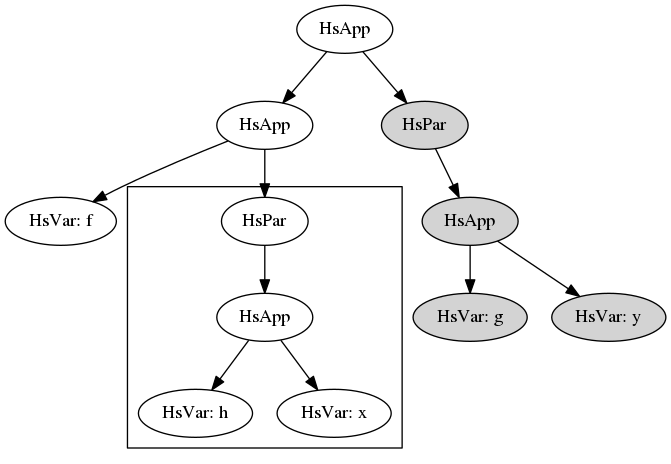
\includegraphics[scale=.5]{graphVis/Chapter6/simpF.png}
	\end{center}
	\caption{The syntax tree of \texttt{f} from figure~\ref{simpleMon}}
	\label{simpF}
\end{figure}

The syntax tree of the right hand side of \texttt{f} is shown in figure~\ref{simpF}. The transformation starts by top down checking the right subtrees for monadic computations. It will first check the call to \texttt{g} (shaded with grey in figure~\ref{simpF}) then it will check the call to \texttt{h} (the corresponding nodes are inside the box). Both of these subtrees are monadic calls so they will be replaced in the tree with unique generated variables. The refactoring implementation contains a queue where the monadic expressions are paired with the variables that replace them and then stored. After this step the expression is \texttt{f v2 v1} and the queue contains two elements \texttt{[(v1,"(g y)"),(v2,"(h x)")]}. The final step checks if the left most child of the current expression is a call to a monadic function. In this case it is because \texttt{f} is a target of the refactoring but if it wasn't then the expression would be composed with \texttt{return}.

At this point the expression is ready to be part of the right hand side of a lambda expression. The first element is popped from the queue, in this case it's \texttt{(v1,"(g y)")}, the variable name becomes the argument in a lambda expression and the expression is the left argument to bind, \texttt{(g y) >>=(\v1 -> f v2 v1)}. In this manner the refactoring keeps popping elements off of the queue wrapping the previous expression in a lambda with the variable name as its argument and composing this lambda with the expression from the queue using bind until the queue is empty.

The final result of refactoring \texttt{f} is shown in figure~\ref{simpF_ref}.

\begin{figure}[t]
\begin{lstlisting}
f x y = (g x) >>= (\ v2 -> (g y) >>= (\v1 -> f v2 v1))
\end{lstlisting}
\caption{The final refactored version of \texttt{f}}
\label{simpF_ref}
\end{figure}

\section{Let Expressions}

The previous section details how the refactoring works over simple function applications. This section will describe how a function with a let expression is refactored. This section will use the expression evaluator in figure~\ref{evalExpr} as a motivating example.

\begin{figure}[t]
\begin{lstlisting}
data Expr = Var Char
          | N Int
          | Add Expr Expr
          | Sub Expr Expr
          | Assign Char Expr
          deriving Show

type Env = [(Char,Int)]

eval :: Expr -> Env -> (Int,Env)

eval (Var v) env = (head [val | (x,val) <- env, x==v], env)

eval (N n) env = (n,env)

eval (Add e1 e2) env = let (v1,env1) = eval e1 env
                                    (v2,env2) = eval e2 env1 
                           in (v1+v2,env2)
eval (Sub e1 e2) env = let (v1,env1) = eval e1 env
                                    (v2,env2) = eval e2 env1 
                           in (v1-v2,env2)
eval (Assign x e) env = let (v,env1) = eval e env 
	in (v, (x,v):env1)
\end{lstlisting}
\caption{An expression evaluator.}
\label{evalExpr}
\end{figure}

The idea is that at this point in the project the explicit passing of the state is unwanted so refactoring \texttt{eval} to become monadic so that the \texttt{Env} can be passed around using the \texttt{State} monad instead. The first two cases that handle the \texttt{Var} and \texttt{N} constructors can simply be wrapped with \texttt{return} because no recursive calls to \texttt{eval} happen in those cases. The three other cases contain let bindings that all call (the now monadic) \texttt{eval}. 

In those cases the local bindings can be used as the variables inside of a lambda expression. This seems simple enough but what order should the bindings be processed in? Consider the let binding in figure~\ref{intLet}, assuming that the \texttt{f} and \texttt{x} variables are in scope, due to lazy evaluation this is a valid Haskell let binding despite \texttt{v1} being referenced on line one before it's defined on line two. However if the let bindings are processed in the obvious way from top to bottom\footnote{In this case: \texttt{g v1 >>= ($\backslash$v2 -> f x >>= ($\backslash$v1 -> ...))}} \texttt{v1} will not be in scope when it's passed to \texttt{g}.  

\begin{figure}[t]
\begin{lstlisting}
let v2 = g v1
     v1 = f x
    in ...
\end{lstlisting}
\caption{An interesting let binding}
\label{intLet}
\end{figure}

Fortunately GHC offers a solution, the renamer of GHC which checks for lexical errors also does dependency analysis on local bindings and orders them so that later bindings may depend on earlier ones but not vice versa~\citep{ghcApi}. This renamed ordering is used to lookup the parsed bindings in dependency analysed order.

Returning to the evaluator example the monadified version is shown in figure~\ref{monEval}.\footnote{Line breaks have been added to aid readability in this setting but the refactoring would not actually do this.} The let bindings in \texttt{eval} can be processed from top to bottom. In the \texttt{Add} case this means that the expression bound on line 16 in figure~\ref{evalExpr} makes up the outermost call to bind and the pattern it was originally bound to becomes the pattern that matches the argument passed to the first lambda expression. 
\begin{figure}[t]
\begin{lstlisting}
eval :: Monad m => Expr -> Env -> m (Int,Env)

eval (Var v) env = return (head [val | (x,val) <- env, x==v], env)

eval (N n) env = return (n,env)

eval (Add e1 e2) env = eval e1 env >>= 
	(\(v1,env1) -> eval e2 env1 >>= 
		(\(v2,env2) -> return (v1+v2,env2)))

eval (Sub e1 e2) env = eval e1 env >>= 
	(\(v1,env1) -> eval e2 env1 >>= 
		(\(v2,env2) -> return (v1-v2,env2)))

eval (Assign x e) env = eval e env >>= 
	(\(v,env1) -> return (v, (x,v):env1)))
\end{lstlisting}
\caption{The monadified expression evaluator.}
\label{monEval}
\end{figure}

If there were pure expressions on the right hand side of the let binding those bindings will remain in a let expression. For example the function starting on line one in figure~\ref{mixLet} contains two let bindings \texttt{pureF} is a pure function and so it remains inside of a let expression whereas \texttt{monF} is a target of the refactoring and it is lifted from the let and passed to bind. 

\begin{figure}[t]
\begin{lstlisting}
f x = let y = pureF x
             z = monF y
		     in z+x

f_m x = let y = pureF x in
		monF y >>= (\z -> return z+x)
\end{lstlisting}
\caption{A function with a mixture of pure and monadic function calls in a let expression.}
\label{mixLet}
\end{figure}

\section{Adding Syntactic Sugar}

The refactored program from figure~\ref{monEval} is rewritten in a restricted call-by-value monadification style. However, idiomatic monadic Haskell is not often written in this style. Haskell also supports a piece of syntactic sugar called \texttt{do} notation. This notation allows for a series of bind computations to be written in a more compact and easier to read style. Figure~\ref{doEx} shows how the bind expression on line one can be sugared into the do statement on lines four through six.

\begin{figure}[t]
\begin{lstlisting}
m_expr >>= (\x -> return (f x))
--Sugars to

do
	x <- m_expr
	return (f x)
\end{lstlisting}
\caption{An example of how binds can sugar to \texttt{do} notation.}
\label{doEx}
\end{figure}

\textbf{\texttt{do}} notation is highly used when writing monadic Haskell programs and some texts even introduce it before explaining what monads are (\cite{realWorldHaskell}; \cite{learnYou}). Supporting this syntax is an important feature for a monadification refactoring to be practical. 

The sugaring of bind syntax into \texttt{do} syntax is a separate refactoring in HaRe. This allows for the programmer to choose exactly which functions should be written with \texttt{do} syntax and when functions are clearer remaining as binds. The refactoring takes in a single parameter, the position where the target function is declared. The sugared version of \texttt{eval} from figure~\ref{monEval} is shown in figure~\ref{finEval}. The first two cases weren't bind expressions so they remain just calls to return. The three other cases have been refactored into the equivalent \texttt{do} statements.

\begin{figure}[t]
\begin{lstlisting}
eval :: Monad m => Expr -> Env -> m (Int,Env)

eval (Var v) env = return (head [val | (x,val) <- env, x==v], env)

eval (N n) env = return (n,env)

eval (Add e1 e2) env = do
	(v1,env1) <- eval e1 env
	(v2,env2) <- eval e2 env1
	return (v1+v2,env2)

eval (Sub e1 e2) env = do
	(v1,env1) <- eval e1 env 
	(v2,env2) <- eval e2 env1
	return (v1-v2,env2)

eval (Assign x e) env = do
	(v,env1) <- eval e env
	return (v, (x,v):env1))
\end{lstlisting}
\caption{The sugared evaluator.}
\label{finEval}
\end{figure}

Monads are a challenging and characteristic feature of Haskell and, anecdotally, infamous amongst those trying to learn the language. Monadification is an important and common transformation that Haskell code undergoes. This chapter has described two refactorings that automate this transformation. The monadification refactoring transforms a set of functions into restricted call-by-value monad style, where only the result type of a function is made monadic. The second refactoring sugars the binds produced by the monadification into \texttt{do} notation, a common structure for monadic Haskell functions.



\chapter{Conclusion}
\label{chp:conc}

\section{Summary of Contributions}

This thesis has explored a new category of refactoring for functional programming languages. Data-driven refactorings are transformations that are \textit{driven} by the data types a program uses. The generalisation refactorings, for example, are motivated by a desire to allow programs to be used in more places (e.g. the ``Maybe to MonadPlus'' refactoring) or even to generalise the way a program is evaluated as in the ``monad to applicative'' refactoring where the \texttt{Applicative} typeclass doesn't force sequential evaluation of the arguments to apply (\texttt{<*>}) like bind (\texttt{>>=}), the monad operation, does.

The primary artifacts of this work are my contributions to HaRe and its API. In particular the following contributions have been made:

\begin{itemize}
\item The design and implementation of a set of data-driven refactorings in HaRe. These refactorings are:
	\begin{itemize}
		\item Introduce a Type Synonym, section~\ref{introSyn}
		\item Generalise Maybe to MonadPlus/Monad, Section~\ref{maybeMonadPlus} and Chapter~\ref{chp:generalImp}
		\item List to Hughes List, section~\ref{listToDlist} and chapter~\ref{chp:generalImp}
		\item Generalise Monad to Applicative, chapter~\ref{chp:applicative}
		\item Monadification	, chapter~\ref{chp:monadification}	
	\end{itemize}
\item An API for the creation of embeddable types refactorings, chapter~\ref{chp:generalImp}
\item Enhancements and additions to HaRe's API, see chapter~\ref{chp:generalImp}. The API was extended while developing the refactorings mentioned above.
\begin{itemize}
	\item Functions that perform high level, common transformations, that many refactorings must do (e.g. wrapping a syntax element in parenthesis)
	\item Functions for retrieving particular syntax elements from the tree of an entire module such as getting the body of a function based on a position.
	\item Functions that aid in working with ghc-exactprint and the annotations such as changing the location of a syntax element relative to the prior syntax element or adding new annotations to a syntax element.
\end{itemize}	  
\end{itemize}
\section{Future Work}
This work and HaRe can be extended in multiple ways. Development on HaRe is ongoing and will continue for the foreseeable future. 

\textit{\textbf{Reimplement Refactorings}} - When HaRe was updated to work with GHC the original implementations of the refactorings were no longer valid using the new back-end. An important task in the near future will be to go back an reimplement the refactorings that are currently not supported in HaRe.  

\textit{\textbf{haskell-ide-engine}} - Alan Zimmerman a major contributor to HaRe is currently working on a new project called the \textit{haskell-ide-engine}\footnote{\url{https://github.com/haskell/haskell-ide-engine}} which will allow Haskell tools to be integrated into IDEs via the Language Server Protocol a standard method of communication between tools and development environments~\citep{lsp}. This project will allow for HaRe to be easily integrated into multiple environments including, Eclipse, Visual Studio Code, Sublime Text, Atom, and Emacs.

\textit{\textbf{Interactive refactorings}} - Many of the more complex refactorings would benefit from becoming more interactive. For example if after the ``introduce type synonym'' refactoring was finished if HaRe you highlight different instances of the type that the synonym was introduced for and ask the user if that instance of the type should be renamed using the new synonym or not. Another possible interactive feature of a refactoring would be to offer to refactor some code if it failed the preconditions for another refactoring. For example, if when trying to refactor a \texttt{do} block to use applicative operations the block fails the precondition requiring that all left hand side variables not be used in a right hand side expression, HaRe could suggest extracting the monadic code into its own function and then performing the original refactoring on the modified function.

\textit{\textbf{Template language for refactoring}} - A powerful feature of Wrangler is its template language~\citep{letsUser}. This allows for Wrangler refactorings to be defined using concrete Erlang syntax rather than the abstract syntax, lowering the difficulty in implementing refactorings significantly for programmers not familiar with the Erlang backend. A similar feature for HaRe would allow refactorings to be written without having to understand the syntax tree of GHC. Template Haskell is a template language for Haskell and is built into the GHC. Unfortunately Template Haskell uses it's own abstract syntax for Haskell code which makes it difficult to use for refactoring GHC Haskell. However, there is a plan to change this though it is not finished yet~\citep{ghcTreesGrow}.

\bibliography{main}

% This index section is optional, use cleardoublepage and phantomsection to make the links work in your contents page. Uses makeidx package.
\cleardoublepage
\phantomsection
\label{index}
\printindex

\end{document}
